% Options for packages loaded elsewhere
\PassOptionsToPackage{unicode}{hyperref}
\PassOptionsToPackage{hyphens}{url}
%
\documentclass[
  11pt,
  openany]{memoir}
\title{The Association Between Travel Behavior and Urban Form}
\author{Shen Qu}
\date{2021-10-15}

\usepackage{amsmath,amssymb}
\usepackage{lmodern}
\usepackage{iftex}
\ifPDFTeX
  \usepackage[T1]{fontenc}
  \usepackage[utf8]{inputenc}
  \usepackage{textcomp} % provide euro and other symbols
\else % if luatex or xetex
  \usepackage{unicode-math}
  \defaultfontfeatures{Scale=MatchLowercase}
  \defaultfontfeatures[\rmfamily]{Ligatures=TeX,Scale=1}
\fi
% Use upquote if available, for straight quotes in verbatim environments
\IfFileExists{upquote.sty}{\usepackage{upquote}}{}
\IfFileExists{microtype.sty}{% use microtype if available
  \usepackage[]{microtype}
  \UseMicrotypeSet[protrusion]{basicmath} % disable protrusion for tt fonts
}{}
\makeatletter
\@ifundefined{KOMAClassName}{% if non-KOMA class
  \IfFileExists{parskip.sty}{%
    \usepackage{parskip}
  }{% else
    \setlength{\parindent}{0pt}
    \setlength{\parskip}{6pt plus 2pt minus 1pt}}
}{% if KOMA class
  \KOMAoptions{parskip=half}}
\makeatother
\usepackage{xcolor}
\IfFileExists{xurl.sty}{\usepackage{xurl}}{} % add URL line breaks if available
\IfFileExists{bookmark.sty}{\usepackage{bookmark}}{\usepackage{hyperref}}
\hypersetup{
  pdftitle={The Association Between Travel Behavior and Urban Form},
  pdfauthor={Shen Qu},
  pdfkeywords={travel behavior, urban form, regression analysis},
  hidelinks,
  pdfcreator={LaTeX via pandoc}}
\urlstyle{same} % disable monospaced font for URLs
\usepackage[margin=1in]{geometry}
\usepackage{longtable,booktabs,array}
\usepackage{calc} % for calculating minipage widths
% Correct order of tables after \paragraph or \subparagraph
\usepackage{etoolbox}
\makeatletter
\patchcmd\longtable{\par}{\if@noskipsec\mbox{}\fi\par}{}{}
\makeatother
% Allow footnotes in longtable head/foot
\IfFileExists{footnotehyper.sty}{\usepackage{footnotehyper}}{\usepackage{footnote}}
\makesavenoteenv{longtable}
\usepackage{graphicx}
\makeatletter
\def\maxwidth{\ifdim\Gin@nat@width>\linewidth\linewidth\else\Gin@nat@width\fi}
\def\maxheight{\ifdim\Gin@nat@height>\textheight\textheight\else\Gin@nat@height\fi}
\makeatother
% Scale images if necessary, so that they will not overflow the page
% margins by default, and it is still possible to overwrite the defaults
% using explicit options in \includegraphics[width, height, ...]{}
\setkeys{Gin}{width=\maxwidth,height=\maxheight,keepaspectratio}
% Set default figure placement to htbp
\makeatletter
\def\fps@figure{htbp}
\makeatother
\setlength{\emergencystretch}{3em} % prevent overfull lines
\providecommand{\tightlist}{%
  \setlength{\itemsep}{0pt}\setlength{\parskip}{0pt}}
\setcounter{secnumdepth}{5}
\newlength{\cslhangindent}
\setlength{\cslhangindent}{1.5em}
\newlength{\csllabelwidth}
\setlength{\csllabelwidth}{3em}
\newlength{\cslentryspacingunit} % times entry-spacing
\setlength{\cslentryspacingunit}{\parskip}
\newenvironment{CSLReferences}[2] % #1 hanging-ident, #2 entry spacing
 {% don't indent paragraphs
  \setlength{\parindent}{0pt}
  % turn on hanging indent if param 1 is 1
  \ifodd #1
  \let\oldpar\par
  \def\par{\hangindent=\cslhangindent\oldpar}
  \fi
  % set entry spacing
  \setlength{\parskip}{#2\cslentryspacingunit}
 }%
 {}
\usepackage{calc}
\newcommand{\CSLBlock}[1]{#1\hfill\break}
\newcommand{\CSLLeftMargin}[1]{\parbox[t]{\csllabelwidth}{#1}}
\newcommand{\CSLRightInline}[1]{\parbox[t]{\linewidth - \csllabelwidth}{#1}\break}
\newcommand{\CSLIndent}[1]{\hspace{\cslhangindent}#1}
\usepackage{amssymb}
\usepackage{amsmath}
\usepackage{subfig}
\usepackage{multicol}
\usepackage{multirow}
\ifLuaTeX
  \usepackage{selnolig}  % disable illegal ligatures
\fi

\begin{document}
\maketitle

{
\setcounter{tocdepth}{1}
\tableofcontents
}
\hypertarget{preface}{%
\chapter*{Preface}\label{preface}}
\addcontentsline{toc}{chapter}{Preface}

This field paper is for discussing the relationship between travel behavior and urban form.\footnote{This is a field paper using the \textbf{bookdown} package (\protect\hyperlink{ref-R-bookdown}{Xie 2021}), \textbf{knitr} (\protect\hyperlink{ref-xie2015}{Xie 2015}) and TinyTeX: \url{https://yihui.name/tinytex/}.}
Part I reviews the related literature and tries to cover the main theories and research in this field.
Daily Driving Distance as the variable of interest, is associated with many factors including urban form variables.
The discussion will gradually narrow down to the association between driving distance and urban density.
Instead of using very high dimension model or synthesized index,
Population Density itself may have more potential to explain the driving distance than people ever thought about.

Part II introduces the linear, generalized linear, and non-linear models which is the fundamental methods for the question raised in Part I.
Meta-analysis is also a useful method to get more general results based on many studies with the same topic.
It can be applied on investigating self-selection and publication bias.

\begin{itemize}
\tightlist
\item
  Several Ideas
\end{itemize}

Many disaggregated travel-urban form models without psychological factors are underfitting, the corresponding estimates are biased.
When the goal of related studies is to provide evidence for public policy, aggregated analysis may be good enough.

The estimated coefficients are incomparable unless the regression models have the common key specification. Because \(\boldsymbol{\hat\beta}=(\mathbf{X'X})^{-1}\mathbf{X'}\mathbf{y}\) is a function depending on \(\mathbf{X}\).
Standardized coefficients or elasticities cannot fix this issues.

Due to the non-linear characteristics of many individual and urban-form factors, identifying the effective ranges of variables is useful for policy making.

\hypertarget{part-part-i-theories-and-framework}{%
\part*{Part I Theories and Framework}\label{part-part-i-theories-and-framework}}
\addcontentsline{toc}{part}{Part I Theories and Framework}

\hypertarget{intro}{%
\chapter{Introduction}\label{intro}}

\hypertarget{background}{%
\section{Background}\label{background}}

In the past decades, efforts have been made to reduce Automobile Dependency in both developed and developing counties. Many research have found that moderating the car use have positive social, economic and environmental impacts. The negative externalities of automobile include, but are not limited to, congestion, collision, unhealthy lifestyle, urban sprawl, social segmentation, pollution, and Greenhouse Gas (GHG) emissions.

In urban planning and transportation, achieving this goal requires two parts. First, researcher find a set of factors which could mostly explain and affect travel behavior. Second, planning and policy are made to intervene the adjustable factors then to reduce the car use significantly.
This paper focuses on the first part and aims at supporting the second part.

\hypertarget{analytical-framework}{%
\section{Analytical Framework}\label{analytical-framework}}

\protect\hyperlink{ref-handyCriticalAssessmentLiterature2005}{Handy} (\protect\hyperlink{ref-handyCriticalAssessmentLiterature2005}{2005}) gives a complete assessment for travel-urban form study, which is the mainstream framework in this field.
Under this framework, regression analysis currently is still the dominate method for explaining the relationship between urban form and travel.
A large mount of studies use regression models to identify the influencing factors and evaluate the effect size. Previous research demonstrated that there is not a single factor determining travel behavior. When choosing continues response, like Vehicle Miles Traveled (VMT),\footnote{or Vehicle Kilometers Traveled (VKT)} the basic structure of the regression model is as below:

\begin{equation}
\mathbf{Y}=\mathbf{X}\boldsymbol{\beta}+\boldsymbol{\varepsilon}
\label{eq:lm}
\end{equation}

where \(\mathbf{Y}\) are the variable of VMT. \(\mathbf{X}\) are all relevant covariates with corresponding coefficients \(\boldsymbol{\beta}\). \(\boldsymbol{\varepsilon}\) are a random error term with expected value of \(0\) and variance \(\sigma^2\).

When the response is categorical variable, such as binary data of driving versus not, polytomous data of mode choice, or count data of trip frequency, the proper model is:

\begin{equation}
E[\mathbf{Y}|\mathbf{X}]=\mu=g^{-1}(\mathbf{X}\boldsymbol{\beta})
\label{eq:glm}
\end{equation}

Where \(E[\mathbf{Y}|\mathbf{X}]\) is the expected value of travel choice variable \(\mathbf{Y}\) conditional on \(\mathbf{X}\); \(\mathbf{X}\boldsymbol{\beta}\) is a linear combination (Ditto.); \(g(\cdot)\) is a link function.

\hypertarget{content-organization}{%
\section{Content Organization}\label{content-organization}}

Part I introduces the Travel-Urban form studies in recent years.
As the essential parts of regression analysis, independent variables of \protect\hyperlink{form}{Urban Form} and dependent variables of \protect\hyperlink{travel}{Travel} are presented using two separate chapters.

Chapter 2 of \protect\hyperlink{form}{Urban Form} starts from a fundamental question: What is the relationship between urban form and travel? How strong the relationship is?
Then the significant influencing factors in literature are systematically introduced.

Aggregated and disaggregated data at vary \protect\hyperlink{scale}{Spatial Scales} can sway the meaning of influencing factors. Units and spatial scales should be careful chosen to make sure the results matching the initial research questions.

Chapter 3, \protect\hyperlink{travel}{the theories of travel behavior} can be divided into \protect\hyperlink{traveler-choice}{Traveler Choice} and \protect\hyperlink{human-mobility}{Human Mobility} by looking travel as object or subject.
These theories and practice can enrich the understanding of travel variable as response of model.

\protect\hyperlink{struc}{Chapter 4} presents several common model structures in existing literature of this field. It demonstrate the different perspectives of the relationship between urban form and travel. Some new trends and methods are also included in this chapter.

\hypertarget{form}{%
\chapter{Urban Form as Predictors}\label{form}}

The concepts of `urban form,' `built environment,' and `land use' are often exchangeable in literature. Adopted from some common usages, here, `urban form' refers to the comprehensive physical expression of land use at the macro scale.\\
`Built environment' emphasizes the urban form attributes as a series of external factors with respect to travelers' internal characteristics and is often used in disaggregated studies at mesoscale. When using `urban form' and `built environment,' one looks at them as the given conditions of travel decision. While `land use' can represent either current status descriptions or designated future use at mesoscale and micro scales.

\hypertarget{influencing-direction}{%
\section{Influencing Direction}\label{influencing-direction}}

Before discussing the impact of land use on travel, the first question is whether land-use characteristics affect the outcome of travel behavior? Or the affecting direction is opposite? Technically, randomized control experiments can identify the causal relationship between them. But in real life, it is impossible to set up some experimental areas and randomly assign people to live in these areas.

Another way is to observe the dynamic of these factors to figure out the direction of influences. \protect\hyperlink{ref-mullerTransportationUrbanForm2004}{Muller} (\protect\hyperlink{ref-mullerTransportationUrbanForm2004}{2004}) reviews the evolution of the U.S. urban form and describe the four eras of intrametropolitan growth (Figure \ref{4age}) in U.S. history: the walking-horsecar era (1800s -- 1890s), the electric streetcar or transit era (1890s -- 1920s), the recreational automobile era (1930s -- 1950s), and the freeway era (1950s -- 2010s) (\protect\hyperlink{ref-rodrigueGeographyTransportSystems2016}{Rodrigue, Comtois, and Slack 2016}). Each four-stage urban transportation development has its dominated spatial structure, which is hard represented by other socio-economic concepts. Each era has a distinctive travel mode, range of distance, and land-use patterns. People can see that the innovation of transportation technology is a determining constraint to other factors and a main driving force to launch the next era.

\begin{figure}

{\centering 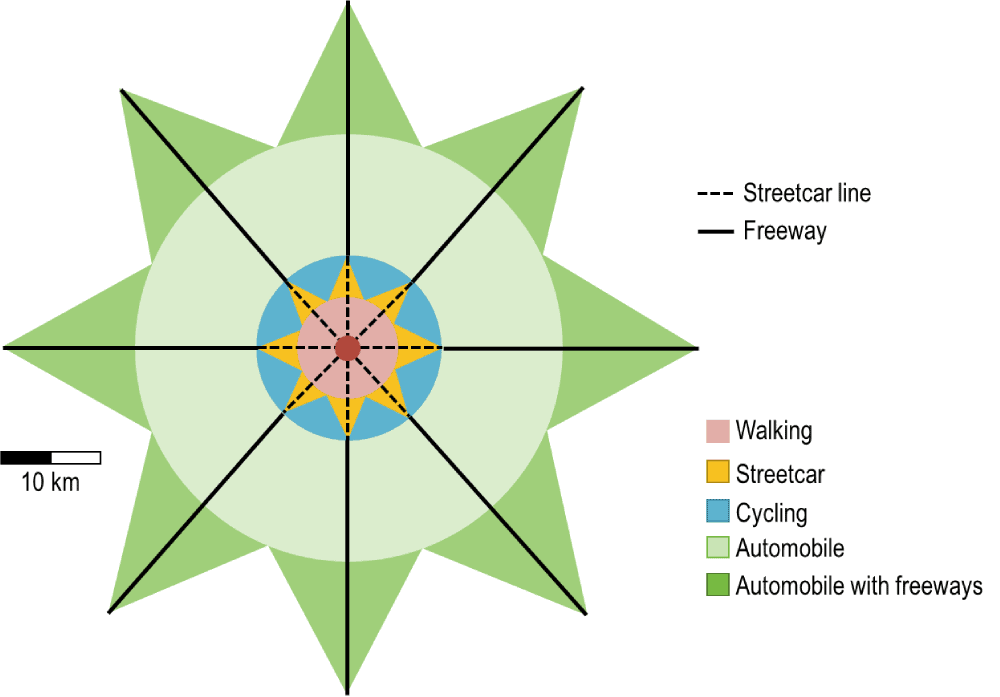
\includegraphics[width=0.5\linewidth]{fig/one_hour_commmuting2} 

}

\caption{One Hour Commuting According to Different Urban Transportation Modes. Source: P.Hugill (1995), World Trade since 1431, p. 213.}\label{fig:4age}
\end{figure}

New transportation tools shifted people's travel modes, extended travel distance, and reshaped the urban form. In causal inference, the new tools are called confounder or common cause, affecting both treatment and outcome. But what is the relationship between travel and urban form? A simple way is to observe the sequence of events to happen. In each transition period, the new tools and new modes began ahead of the new urban development. Even today, multiple travel modes exist in the old town, but suburban seldom has the old way like the streetcar. Thus, urban form is more like an outcome rather than treatment.

However, the urban form remains relatively more stable than an individual's travel behavior in each era. A family may be used to driving in Texas and turn to use the subway when they move to New York and vice versa. Given a period, VMT could be affected by density and other factors. It doesn't make sense that VMT will change the density in the short term. Therefore, urban form can be treated as independent variables in the context of the current stage of urban development. The relationship of urban form with respect to travel can hold for a period of time.

Over the long term, the relationships among travel, urban form, and other physical, socio-economic, demographic factors were interactive and iterative. \protect\hyperlink{ref-levinsonMetropolitanTransportLand2018}{D. M. Levinson and Krizek} (\protect\hyperlink{ref-levinsonMetropolitanTransportLand2018}{2018}) emphasize transportation is a necessary but not a sufficient factor for any development. The change of eras is a comprehensive outcome of socio-economic and technological development. Which factor caused which effect does not have a simple answer. A conservative view is that land use and travel behavior are determined simultaneously by the transportation costs (\protect\hyperlink{ref-pickrellTRANSPORTATIONLANDUSE1999}{Pickrell 1999}).

Although randomized control experiments about travel and urban form are impossible, the regression model can still explore their associations once the simultaneous relationship holds.

\hypertarget{influencing-factors}{%
\section{Influencing Factors}\label{influencing-factors}}

For the complexity of travel behavior, many objective or subjective factors could change people's travel decisions. They include but are not limited to physical, socio-demographic, individual, and policy determinants. It seems impossible to make an exhaustive list. Here briefly introduces several significant influencing factors.

A dichotomy of individual versus environmental factors is a common framework. All relevant factors involving personal or household characteristics can be categorized as internal factors. In comparison, the built environment and other environmental factors have external influences. Disaggregate analysis usually chooses this structure because the models can distinguish the different sources of variation from individual and environmental factors. For example, the VMT model is as follows.

\[\begin{aligned}
\mathbf{Y}=\mathbf{X}_\mathrm{I}\boldsymbol{\beta}_\mathrm{I}+\mathbf{X}_\mathrm{E}\boldsymbol{\beta}_\mathrm{E}+\boldsymbol{\varepsilon}
\end{aligned}\]

where \(\mathbf{X}_\mathrm{I}\) are travelers' internal characteristics; \(\mathbf{X}_\mathrm{E}\) are built environment and other environment covariates.

\hypertarget{individual-factors}{%
\subsection{Individual Factors}\label{individual-factors}}

Previous research have identified many internal factors have strong impact on travel.\\
Vehicle ownership is a good indicator for choosing auto mode and longer travel distance (van der Waard, Jorritsma, and Immers 2013). Employment status or entry into the labor market often increases driving while retirement may have more walking or cycling for fewer time constraints. (Goodwin and Van Dender, 2013; Grimal, Collet, and Madre, 2013; Headicar, 2013)

Some factors shows significant impact on travel but give opposite directions. Sometimes, it implies some nonlinear features. For example, income usually has a positive relationship with car ownership and driving distance. But some studies find less-wealthy groups have more cars and longer driving distance (Goetzke and Weinberger 2012). Sometimes, it depends on the location and social background. Dargay and Hanly (2007) find the number of children in household has a positive relationship in the U.K. While Ding et al.~(2017) find a negative effect in the U.S.

\protect\hyperlink{ref-laroucheEffectMajorLife2020}{Larouche et al.} (\protect\hyperlink{ref-laroucheEffectMajorLife2020}{2020}) make a scoping review of some major life events on travel behavior. They provide some explanation for the inconsistent results. Relocation provide windows of opportunity for travel behavior change, but the direction depend on people's attitude. Psychological factors such as travelers' habits and preferences are determinant. Similarly, the choice after school transitions depends on the new environmental factors. Marriage is not significant because couples may live together before marriage. In a similar way, parents may have more car use several years after childbirth for the purposes of childcare, school, recreation, etc.

Therefore, a well performed model should contain these influencing factors to increase models' fitness. Controlling these independent variables, which can not be intervened by policy, can help to identify how large the effect sizes of adjustable factors are. These studies also notes that the range, location, and understanding of internal variables are critical for a proper model.

\hypertarget{environmental-factors}{%
\subsection{Environmental Factors}\label{environmental-factors}}

Environmental factors usually impact a large number of people. Three main categories are natural environment, socio-economic environment, and built environment. The natural terrain, temperature, and precipitation could change travelers' choice. These factors can only be examined across cities and regions. They are also hard to change and are not included in many studies.

Socio-economic environment such as fuel price and crime rates also encourage/discourage people choosing driving for economic or safety reasons. Some of them, such as car culture are hard to measure and control as other psychological factors. Some factors could be related to the broader topics such as quality of life, or public security. In these cases car usage is not the core concerns.

Infrastructure supplement is also a set of strong explanatory variables. It has been proven that road capacity and parking space are two primary factors for driving. The problem is that reducing supply is painful for public and is subject to political pressure. Increasing and improving transit services are more attractive through providing a substitution of driving (Kuhnimhof, Zumkeller, and Chlond 2013).

Policy environment as treatment applied on a administrative region, such as restrictions on car use, can only be examined by comparing with the `control groups.' Meanwhile, transportation policy is a context-dependent factor. The same policy in name may be implemented in very different ways across the country. Cross-sectional study is a challenge because existing the complex interaction effects between a policy and the characteristics of the `experimental group.' Longitudinal study and Difference in Difference (DID) methods are more common in policy evaluations. There are also two types of policies. Travel Demand Management (TDM) heads directly toward change of travel behavior. For example, studies find parking management and low ticket fare by subsidies can attract more transit passengers (Grimal, Collet, and Madre 2013). While many urban development policies such as UBG, TOD, and rezoning have more comprehensive goals.

Built environment such as urban density and design is a primary focus of attention in urban studies because they are more changeable than natural environment. They are simple and measurable for implement. They are more acceptable for neutral meaning and can change people's behavior inadvertently.

policy or planning might be able to intervene current and future land use, further achieve the goal of travel behavior change. ``Attributes of the built environment influence travel by making travel to opportunities more or less convenient and attractive'' (\protect\hyperlink{ref-domencichURBANTRAVELDEMAND1975}{Domencich and McFadden 1975}; \protect\hyperlink{ref-levinsonElementsAccessTransport2017}{D. M. Levinson, Marshall, and Axhausen 2017}; \protect\hyperlink{ref-litmanHowLandUse2017}{Litman 2017}). There are many complex unknown interaction effects between built-environment and other variables. Some research found that the habit discontinuity hypothesis, major life events may provide windows of opportunity during which individuals may reconsider their travel behaviors and be more sensitive to behavior change interventions (\protect\hyperlink{ref-verplankenContextChangeTravel2008}{Verplanken et al. 2008}). The changes in built-environment attributes may capture these windows of opportunity. Further introduction is placed in the next section.

\hypertarget{density}{%
\subsection{Density}\label{density}}

Density is the first built-environment factor added to the model. Early research of automobile trips and urban density can go back sixty years (\protect\hyperlink{ref-mitchellUrbanTraffic1954}{Mitchell and Rapkin 1954}). \protect\hyperlink{ref-levinsonEFFECTSDENSITYURBAN1963}{H. S. Levinson and Wynn} (\protect\hyperlink{ref-levinsonEFFECTSDENSITYURBAN1963}{1963}) suggest that the people who lived in high-density neighborhoods make fewer automobile trips. This argument stimulated an enormous volume of work. Although later studies construct more complex models, density factor stays in most of travel-urban form model even today.

The most influential aggregate studies start from Newman and Kenworthy. They published a series of studies to show a strong negative correlation between per capita fuel use and gross population density (GPD).\footnote{\protect\hyperlink{ref-newmanCITIESAUTOMOBILEDEPENDENCE1989}{P. G. Newman and Kenworthy} (\protect\hyperlink{ref-newmanCITIESAUTOMOBILEDEPENDENCE1989}{1989a});\protect\hyperlink{ref-newmanGasolineConsumptionCities1989}{P. G. Newman and Kenworthy} (\protect\hyperlink{ref-newmanGasolineConsumptionCities1989}{1989b});\protect\hyperlink{ref-kenworthyINTERNATIONALSOURCEBOOKAUTOMOBILE1999}{J. R. Kenworthy et al.} (\protect\hyperlink{ref-kenworthyINTERNATIONALSOURCEBOOKAUTOMOBILE1999}{1999});\protect\hyperlink{ref-newmanUrbanDesignReduce2006}{P. Newman et al.} (\protect\hyperlink{ref-newmanUrbanDesignReduce2006}{2006});\protect\hyperlink{ref-newmanPeakCarUse2011}{P. Newman and Kenworthy} (\protect\hyperlink{ref-newmanPeakCarUse2011}{2011a});\protect\hyperlink{ref-newmanDensityMultiplierResponse2011}{P. Newman and Kenworthy} (\protect\hyperlink{ref-newmanDensityMultiplierResponse2011}{2011b});\protect\hyperlink{ref-newmanDensitySustainabilityMultiplier2014}{P. Newman} (\protect\hyperlink{ref-newmanDensitySustainabilityMultiplier2014}{2014});\protect\hyperlink{ref-newmanEndAutomobileDependence2015}{P. Newman and Kenworthy} (\protect\hyperlink{ref-newmanEndAutomobileDependence2015}{2015});\protect\hyperlink{ref-kenworthyAutomobileDependenceEmerging2017}{Jeffrey R. Kenworthy} (\protect\hyperlink{ref-kenworthyAutomobileDependenceEmerging2017}{2017})} Their sample covers from thirty-two to fifty-eight global cities (\protect\hyperlink{ref-newmanCITIESAUTOMOBILEDEPENDENCE1989}{P. G. Newman and Kenworthy 1989a}; \protect\hyperlink{ref-newmanEndAutomobileDependence2015}{P. Newman and Kenworthy 2015}) and produced very convincing results. Their research points out the relationship rather than estimating the effect size. In this way, the denser cities have less fuel consumption, which implies less automobile dependence. This is a succinct argument and is widely accepted by planners and policy makers.

The criticisms include their ideological grounds, dataset, and model specification(\protect\hyperlink{ref-gordonGasolineConsumptionCities1989}{Gordon and Richardson 1989}; \protect\hyperlink{ref-dujardinHometoworkCommutingUrban2012}{Dujardin et al. 2012}; \protect\hyperlink{ref-perumalContextualDensityUS2017}{Perumal and Timmons 2017}). A criticism is that, for aggregated data, the population variable on both sides of the equation artificially creates a hyperbolic function (Equation \eqref{eq:hyperbolic}). In many disaggregated studies, the effects of density are not significant and have a small magnitude (\protect\hyperlink{ref-zhaoRethinkingDeterminantsVehicle2021}{Zhao and Li 2021}).

\begin{equation}
\begin{split}
 & \text{VMT}_{average}  =\beta\cdot  \text{Density}  +\cdots\\ 
\implies & \frac{\text{VMT}_{total}}{\text{Population}}  = \beta\cdot  \frac{\text{Population}}{\text{Area}}  +\cdots\\
\implies & \text{VMT}_{total} = \beta\cdot  \frac{(\text{Population})^2}{\text{Area}}  +\cdots
\end{split}
\label{eq:hyperbolic}
\end{equation}

Another criticism argues that the global comparisons are not valid, such as comparing Hong Kong and Houston. \protect\hyperlink{ref-ewingTestingNewmanKenworthy2018}{Ewing et al.} (\protect\hyperlink{ref-ewingTestingNewmanKenworthy2018}{2018}) created a subset with only U.S. Metropolitan areas from \protect\hyperlink{ref-kenworthyPatternsAutomobileDependence1999}{Jeffrey R. Kenworthy and Laube} (\protect\hyperlink{ref-kenworthyPatternsAutomobileDependence1999}{1999}) `s original data set. They fit the same model but get a much lower \(R^2\) (0.096) than Kenworthy and Laube's (0.72). A similar work by \protect\hyperlink{ref-fanisThreeStudiesThat2019}{Fanis} (\protect\hyperlink{ref-fanisThreeStudiesThat2019}{2019}) shows the low \(R^2\) for U.S. cities (0.1838) and European cities (0.2804) when deconstructing Newman and Kenworthy's data by continent. Actually, any research question has its corresponding sampling design. Choosing a cutoff from the whole data often gets a different result. These criticisms are unfair for Kenworthy and Laube's work. But it is true that U.S. cities have higher VMT and lower density than other countries' cities. Recent evidence over a 20-year period from other cities and counties show that the status quo of the U.S. only represents a small window of the global trend(\protect\hyperlink{ref-kenworthyAutomobileDependenceEmerging2017}{Jeffrey R. Kenworthy 2017}).

Density variable have some advantages. Density is calculated by population size and area size from census data, which are widely available over the country. In contrast, some individual variables are not as measurable and accurate as density. Some studies found density might be an intermediate variable or proxy to other land use variables such as land use mix, street network, and transit services (\protect\hyperlink{ref-ewingTravelBuiltEnvironment2010}{Ewing and Cervero 2010}; \protect\hyperlink{ref-handyCriticalAssessmentLiterature2005}{Handy 2005}). The divisions of the statistical units in the U.S. are from an uniform criteria at multiple scales. Thus, density values is more objective, and comparable comparing other measurements.

Density is an informative factor. Except for the mean and variance, The moments function for Urban density such as skewness, kurtosis, or rank, all can be the predictor candidates. Scolar also explore more delicate measurements of density such as Propotional Weighted Density to replace overall density. ``population-weighted density is equal to conventional density plus the variance of density across the subareas used for its calculation divided by the conventional density'' (\protect\hyperlink{ref-ottensmannPopulationWeightedDensity2018}{Ottensmann 2018}). Some studies use a geographically weighted regression (GWR) (\protect\hyperlink{ref-GeographicallyWeightedRegression}{{``Geographically {Weighted Regression} - an Overview \textbar{} {ScienceDirect Topics}''} n.d.}) procedure to identify significant employment density peaks.

Urban density can be represented by many approximate variables -- built-up density, residential density, employment density, destination density, or CBD density. Here this paper focus on population density -- how many people live in a square mile of land - and involves others if possible.

\hypertarget{d-variables}{%
\subsection{D-variables}\label{d-variables}}

One trenchant criticism of Newman and Kenworthy's work is that the univariate or bivariate models may leave some critical factors out. In a recent debate (\protect\hyperlink{ref-fanisThreeStudiesThat2019}{Fanis 2019}), Newman clarified that ``All our work shows that there are multiple causes of car dependence and multiple implications.'' Since travel behavior is a multi-dimensional issue, more socio-demographic and built-environment variables were added to the multivariate analysis. The work started from adding three `Ds' variables, \emph{density}, \emph{diversity}, and \emph{design} (\protect\hyperlink{ref-cerveroTravelDemand3Ds1997}{Cervero and Kockelman 1997}), extended to five `Ds,' adding \emph{destination accessibility} and \emph{distance to transit} (\protect\hyperlink{ref-ewingTravelBuiltEnvironment2001}{Ewing and Cervero 2001}). It even grows to seven with the addition of \emph{demand management} and \emph{demographics}.

Ds' framework is a significance-centered mixed factor set and has become one of the most influential ideas in travel-built environment literature in the past decades. Using household-level or person-level data, these studies tried to disclose more complex relationships among the candidate factors by adding more relevant variables.

The criticism from \protect\hyperlink{ref-handyEnoughAlreadyLet2018}{Handy} (\protect\hyperlink{ref-handyEnoughAlreadyLet2018}{2018}) says the 5Ds variables may not be independent. A meta-analysis found that spatial multicollinearity is widespread in this field (\protect\hyperlink{ref-gimRelationshipsLandUse2013}{Gim 2013}). Although previous studies usually check multicollinearity issues, these variables still correlate with each other in some ways and may have strong interaction effects.

\hypertarget{synthesized-index}{%
\subsection{Synthesized Index}\label{synthesized-index}}

To address the multicollinearity and interactions issues, \protect\hyperlink{ref-cliftonGettingHereThere2017}{Clifton} (\protect\hyperlink{ref-cliftonGettingHereThere2017}{2017}) suggest to convert the various environmental characteristics to built environment indices. Some research try to use `compactness indices' to replace the single density measurement (\protect\hyperlink{ref-ewingRelationshipUrbanSprawl2014}{Ewing et al. 2014}; \protect\hyperlink{ref-hamidiLongitudinalStudyChanges2014}{Hamidi and Ewing 2014}; \protect\hyperlink{ref-hamidiMeasuringSprawlIts2015}{Hamidi et al. 2015}; \protect\hyperlink{ref-ewingUrbanSprawlRisk2016}{Ewing, Hamidi, and Grace 2016}). The primary method is principal components analysis (PCA) or principal components regression (PCR), which synthesizes many variables to four dimensions: development density, land use mix, activity centering, and street connectivity. The advantage of this method is to increase the elasticity value significantly. A recent study shows that the elasticity of VMT with respect to a county compactness index is -0.78. The disadvantage of this method is that the internal mechanisms of the indices are still not clear. Another disadvantage is that the various indices are not comparable. For example, \protect\hyperlink{ref-zhangHouseholdTripGeneration2019}{Q. Zhang et al.} (\protect\hyperlink{ref-zhangHouseholdTripGeneration2019}{2019}) use urban living infrastructure (ULI) as the local accessibility variable (ULI) and find ULI and household density have significant effects on household trip generation. Their ULI is the count number of retail, services, and social activities. Meanwhile, the Urban Liveability Index (ULI) by \protect\hyperlink{ref-higgsUrbanLiveabilityIndex2019}{Higgs et al.} (\protect\hyperlink{ref-higgsUrbanLiveabilityIndex2019}{2019}) are some indices supporting health and wellbeing. These indices include not only social infrastructure and transit service, but also walkability, public open space, housing, and employment. The two ULIs have different information and may not be comparable. Hence, the association between ULI and travel mode choice is a specific result unless an uniform measurement is widely applied on other studies and cities.

A smart application of synthesize method (common factor analysis) is to control the physiological effects in models. \protect\hyperlink{ref-hongHowBuiltenvironmentFactors2014}{Hong, Shen, and Zhang} (\protect\hyperlink{ref-hongHowBuiltenvironmentFactors2014}{2014}) convert eight attitudinal questions in the 2006 Household Activity Survey to three factors: Ease, Convenience, and Pro-transit. They fit the model using two geographic scales: 1-km buffer and traffic analysis zone (TAZ). After contolling the attitudinal effects, the \emph{nonresidential density} and \emph{distance from CBD} have significant effects on VMT at the TAZ level.

\hypertarget{meta-aanalysis}{%
\section{Meta-Aanalysis}\label{meta-aanalysis}}

This section introduces several influencing meta-analysis of travel-urban form studies. The relevant methods is in a separate chapter of Part II.

\begin{itemize}
\tightlist
\item
  \protect\hyperlink{ref-ewingTravelBuiltEnvironment2010}{Ewing and Cervero} (\protect\hyperlink{ref-ewingTravelBuiltEnvironment2010}{2010})
\end{itemize}

To get a general, comparable outcome, \protect\hyperlink{ref-ewingTravelBuiltEnvironment2010}{Ewing and Cervero} (\protect\hyperlink{ref-ewingTravelBuiltEnvironment2010}{2010}) collected more than 200 related studies and summarized the elasticity values using meta-analysis. They exclude the aggregated studies to avoid ``ecological fallacies.'' The studies on specific groups such as aged people are also excluded. The selected studies must use multiple regression analysis with at least one response of VMT or travel modes, with at least one predictor from 5D variables. The studies using structural equation models are not included because these models will not give a single effects size of each 5D variables. The coefficients with respect to vary metrics of predictors are incomparable. Thus they convert all the estimates of coefficient to elasticities. Elasticity measures the percentage change in response with respect to a 1 percent increase in a predictor. Thus, it is a dimensionless parameter.

After screening, sixty-two studies were selected. This is a very small sample size because the research question involves five predictors (5D-variables) and three responses (VMT, walking, and transit use). Taking the VMT-density relationships for example, there are only nine selected studies in this meta-analysis. It is not large enough to get a sufficient inference. Looking at the distribution of elasticities, six of nine papers gave zero or insignificant elasticity. Three studies showed significant negative values (two are -0.04 and one is -0.12). \protect\hyperlink{ref-ewingTravelBuiltEnvironment2010}{Ewing and Cervero} (\protect\hyperlink{ref-ewingTravelBuiltEnvironment2010}{2010}) use the nine observation to calculate the weighted-average elasticities of VMT with respect to population density. The result of -0.04 is mainly determined by the three observations.

Moreover, among the nine VMT-density studies, eight use single city/metro data. Only one nationwide study using NPTS data (\protect\hyperlink{ref-schimekHouseholdMotorVehicle1996}{Schimek 1996}) finds logarithm of household VMT has a non-significant elasticity (-0.07).

Similarly, in this meta-analysis, the weighted-average elasticity of job density (sample size = 9) was zero. The largest elasticities of VMT are found be -0.20 with respect to job accessibility by auto (sample size = 5) and -0.22 with respect to distance to downtown (sample size = 3).

For the limitation of data quality, the standard error of elasticities are not included in this meta-analysis. When calculating the weighted-average values, \protect\hyperlink{ref-ewingTravelBuiltEnvironment2010}{Ewing and Cervero} (\protect\hyperlink{ref-ewingTravelBuiltEnvironment2010}{2010}) use the sample size of each study as the weight factor. For the same reason, the confidence intervals are also not available.

\begin{table}

\caption{\label{tab:meta2010}The Studies of VMT vresus Density in @ewingTravelBuiltEnvironment2010}
\centering
\fontsize{7}{9}\selectfont
\begin{tabular}[t]{llrl}
\toprule
Study & Sites & Elasticity & note\\
\midrule
@ewing2009measuring & Portland,OR & 0.00 & \\
@frankMultipleImpactsBuilt2005 & Seattle & 0.00 & \\
@greenwald2009sacsim & Sacramento & -0.07 & Non-peer-reviewed;Non-significant\\
@mariakockelmanTravelBehaviorFunction1997 & Bay Area & 0.00 & \\
@kuzmyak2009estimating & Los Angeles & -0.04 & Non-peer-reviewed\\
\addlinespace
@kuzmyak2009estimates & Phoenix & 0.00 & Non-peer-reviewed\\
@zegrasBuiltEnvironmentMotor2010 & Santiago de Chile & -0.04 & \\
@zhouSelfSelectionHomeChoice2008 & Austin & -0.12 & not log transform,\$R\textasciicircum{}2\$=0.097\\
@schimekHouseholdMotorVehicle1996 & U.S. & -0.07 & Non-significant\\
\bottomrule
\end{tabular}
\end{table}

This meta-analysis kindled researchers' enthusiasm for this topic. After that, some studies try to cover multi-region data (\protect\hyperlink{ref-zhangHowBuiltEnvironment2012}{L. Zhang et al. 2012}). \protect\hyperlink{ref-ewingVaryingInfluencesBuilt2015}{Ewing et al.} (\protect\hyperlink{ref-ewingVaryingInfluencesBuilt2015}{2015}) accumulated a travel and built environmental dataset from 23 metropolitan regions in US (81,056 households and 815,204 people). They find that all of the 11 D-variables have statistically significant effects on VMT.

\begin{itemize}
\tightlist
\item
  \protect\hyperlink{ref-stevensDoesCompactDevelopment2017}{Stevens} (\protect\hyperlink{ref-stevensDoesCompactDevelopment2017}{2017a})
\end{itemize}

\protect\hyperlink{ref-stevensDoesCompactDevelopment2017}{Stevens} (\protect\hyperlink{ref-stevensDoesCompactDevelopment2017}{2017a}) extends this analysis and tries to explain the different outcomes using a meta-regression method. He focuses on the studies with VMT as the response and uses similar screening criteria. Based on the results from 37 studies, he finds the elasticity of population density is small (-0.10) and suggest that compacting development has a tiny influence on driving.

By adding a dummy variable, whether a study control residential self-selection or not, into the meta-regression, \protect\hyperlink{ref-stevensDoesCompactDevelopment2017}{Stevens} (\protect\hyperlink{ref-stevensDoesCompactDevelopment2017}{2017a}) shows that self-selection research design could impact the effect size significantly. For the studies with self-selection control, the estimated elasticity of population density becomes -0.22, which is much stronger than \protect\hyperlink{ref-ewingTravelBuiltEnvironment2010}{Ewing and Cervero} (\protect\hyperlink{ref-ewingTravelBuiltEnvironment2010}{2010}) 's result (-0.04). An advantage of meta-regression is the two groups with/without self-selection control can share the common errors, that fully utilizes the information and can overcome the small sample size issue to a certain extent. The number of studies with self-selection control is four, while the totoal selected studies is 19. This results is more reliable than the average value in self-selection control group.

Another improvement is that Stevens' meta-regression uses weighted least squares (WLS) method. The weights are the precision (inverse of variance) of each observation. The same weights are applied on the weighted average and precision-effect estimate with standard error (PEESE) method in his `Technical Appendix for details.' The estimated elasticities of population density with the three methods are -0.22, -0.13, and -0.20 respectively. Unfortunately, Stevens doesn't share any information of standard error of coefficients in the article and technical appendix. It is not easy to check his data and results.

Note that one observation, the study by \protect\hyperlink{ref-chatmanHowDensityMixed2003}{Chatman} (\protect\hyperlink{ref-chatmanHowDensityMixed2003}{2003}) may twist Stevens' result about density dramatically. In Chatman's Tobit model, the average VMT is \(\bar y= 3.988\); the average household density is \(\bar x= 1.902\) (housing units per square mile, residential block group (1,000s)); the coefficient of household density is \(\beta=-0.082\). Then the elasticity should be

\[
\beta\cdot\frac{\bar x}{\bar y}=-0.082\cdot\frac{1.902}{3.988}=-0.0391
\]

This elasticity calculated by \protect\hyperlink{ref-ewingTravelBuiltEnvironment2010}{Ewing and Cervero} (\protect\hyperlink{ref-ewingTravelBuiltEnvironment2010}{2010}) is -0.58. And it is not selected in meta-analysis because the response is VMT on commercial trips. \protect\hyperlink{ref-stevensDoesCompactDevelopment2017}{Stevens} (\protect\hyperlink{ref-stevensDoesCompactDevelopment2017}{2017a}) chooses this study and calculates a different elasticity -0.34. Whatever, -0.34 is the smallest elasticity and the second smallest one (\protect\hyperlink{ref-zahabiSpatiotemporalAnalysisCar2015}{Zahabi et al. 2015}) is -0.22. While the rest studies give the range of elasticities from 0 to -0.20. Hence, these observations is highly skewed.

\protect\hyperlink{ref-chatmanHowDensityMixed2003}{Chatman} (\protect\hyperlink{ref-chatmanHowDensityMixed2003}{2003}) `s model is also the only one of four studies with self-selection control. If remove this case (-0.34), the estimated effect size will be much close to zero. \protect\hyperlink{ref-zahabiSpatiotemporalAnalysisCar2015}{Zahabi et al.} (\protect\hyperlink{ref-zahabiSpatiotemporalAnalysisCar2015}{2015}) has the largest sample size (147574). Steven finds the PEESE method for bias correction will change the weighted average elasticity from -0.13 to -0.20. He hesitates to remove this 'outlier' because the outcome will become -0.09. At last, he choose to keep this observation and report the result without bias correction (-0.22). Changing the criteria after seeing the results is called post hoc analysis, or exploratory analysis.

Stevens' work triggers a round of discussion. In \protect\hyperlink{ref-ewingDoesCompactDevelopment2017}{Ewing and Cervero} (\protect\hyperlink{ref-ewingDoesCompactDevelopment2017}{2017}) `s reply, they don't doubt Stevens' results and criticize his conclusions. They agree with the values of elasticity but argue that Stevens' results (-0.22 for density) are not small actually. They emphasize the extensive benefit of compacting development. They don't think reporting bias is widely exist in built environment-travel studies. The difference results of meta-analysis is mainly duo to the studies selection, such as U.S. or international context. Keeping or removing the outlier is also make the difference.

Other scholars also contribute various insights. \protect\hyperlink{ref-manvilleTravelBuiltEnvironment2017}{Manville} (\protect\hyperlink{ref-manvilleTravelBuiltEnvironment2017}{2017}) supports the idea that compact development are related to less car use and look it as a ``fundamental belief in urban planning.'' \protect\hyperlink{ref-nelsonCompactDevelopmentReduces2017}{Nelson} (\protect\hyperlink{ref-nelsonCompactDevelopmentReduces2017}{2017}) agree that selective reporting bias does exist when some ``interests or ideology dominate the discussion.'' \protect\hyperlink{ref-cliftonGettingHereThere2017}{Clifton} (\protect\hyperlink{ref-cliftonGettingHereThere2017}{2017}) points out some weakness and potential sources of bias in current travel behavior studies. \protect\hyperlink{ref-heresFutureResearchLink2017}{Heres and Niemeier} (\protect\hyperlink{ref-heresFutureResearchLink2017}{2017}) support more application of meta-analysis on relevant studies. And they remind the substantial difference among the studies with vary methods, data sources of country, and metrics (e.g.~commuting and noncommuting trips). They suggest to narrow the scope of studies down to get more specific conclusions for policymakers. \protect\hyperlink{ref-knaapDrivingCompactGrowth2017}{Knaap, Avin, and Fang} (\protect\hyperlink{ref-knaapDrivingCompactGrowth2017}{2017}) provide some suggestions for improving this approach from the perspective of sample size, model specification, and weighing. Among the discussion, a key issue is whether an universal effect of compact development with respect to driving distance exists, or the effect is totally context dependent. If the former is true, Stevens' work should not be criticized for the cross-country scope. If the later is true, it still should be based on evidence rather than belief or experience. The complexity of urban issues makes it being an unsolved problem.

\protect\hyperlink{ref-handyThoughtsMeaningMark2017}{Handy} (\protect\hyperlink{ref-handyThoughtsMeaningMark2017}{2017}) agrees with the improvement by meta-regression but thinks that meta-analysis is not a direction worth to further investigation. In a later paper, \protect\hyperlink{ref-handyEnoughAlreadyLet2018}{Handy} (\protect\hyperlink{ref-handyEnoughAlreadyLet2018}{2018}) argues that the 5Ds framework should be replaced by accessibility-centered studies. In \protect\hyperlink{ref-stevensResponseCommentariesDoes2017}{Stevens} (\protect\hyperlink{ref-stevensResponseCommentariesDoes2017}{2017b}) 's response to commentaries, he clarifies some research goals and important questions. He insists this meta-regression is currently ``most accurate synthesis of the literature.''

Stevens' study shows a uncommon direction of bias on elasticity of population density. An usual assumption of publication bias is small-studies tend to have greater standard errors and effect sizes. In contrast, among the 19 studies including density variable, the effect sizes in small-studies are closer to zero. An possible reason is the studies have high heterogeneity are answering different questions. In a highly heterogeneous field, researcher may not have too much pressure for small effect size. Another possible explanation is that most of recent studies include a bundle of predictors. Once one or more coefficients show significant, the paper will be treated equally. Publication bias only affects the nothing significant studies.

\begin{itemize}
\tightlist
\item
  \protect\hyperlink{ref-astonExploringBuiltEnvironment2021}{Aston et al.} (\protect\hyperlink{ref-astonExploringBuiltEnvironment2021}{2021})
\end{itemize}

After the two milestones for meta-analysis of built environment and travel behavior, a recent update re-examines the post-2010 empirical literature. \protect\hyperlink{ref-astonStudyDesignImpacts2020}{Aston et al.} (\protect\hyperlink{ref-astonStudyDesignImpacts2020}{2020}) collected 146 studies containing 467 models and being recorded as 1662 data points. There are 15 predictors of research design, including the number of variables, aggregate/disaggregate data, general/commuter group, trip purposes, time periods, types of model, are used to examine how research design affects the built environment-mode choice studies. Instead of using elasticities as the response variable, they choose correlation, another dimensionless variable to measure the strength of the relationship between built environment and transit use. Their results shows that whether accounting residential self-selection and regional accessibility can account for 40\% of variation of mode choice in the meta-regression.

Actually, this meta-regression use Stepwise selection method to remove the insignificant predictors. 40\% is the coefficient of determination \(R^2\) in the four-predictor model for density and the five-predictor model for Diversity. In these meta-regression models, standard errors \(SE_r\) show the largest coefficient value. Control for covariance (which lack of explanation in this paper) contributes the second large one. Control for regional accessibility is a insignificant variable in both Density and Diversity models. How can get the conclusion of the 40\% of variation are duo to the control of self-selection and regional accessibility? \protect\hyperlink{ref-astonStudyDesignImpacts2020}{Aston et al.} (\protect\hyperlink{ref-astonStudyDesignImpacts2020}{2020}) mention the asymmetry existed in the funnel plot for density and accessibility. It is an evidence of publication bias that could lead to overestimate the correlation. But the plot is not shown in the paper.

In a later paper, \protect\hyperlink{ref-astonExploringBuiltEnvironment2021}{Aston et al.} (\protect\hyperlink{ref-astonExploringBuiltEnvironment2021}{2021}) further improve the meta-analysis to examine the impacts of 5D variables on transit use. The number of studies are extended to 187. And 418 of 505 elasticities are used as valid response. They find that, using a random-effect model, the elasiticity of density on transit use (0.10) is close to \protect\hyperlink{ref-ewingTravelBuiltEnvironment2010}{Ewing and Cervero} (\protect\hyperlink{ref-ewingTravelBuiltEnvironment2010}{2010}) 's result (0.07). The standard error of estimate is also included \(SE=0.013\). Using this estimites, they re-examine the effects of control for self-selection and regional accessibility. The paired tests show that both of the two indicators have significant effects on elasticities of density. They also find the estimated elasticity of density in the studies after 2010 is significantly higher than the studies before 2010. The authors explain this change by more diverse study locations and more studies which control for regional accessibility after 2010.

\hypertarget{scale}{%
\section{Spatial Scales}\label{scale}}

\hypertarget{modifiable-areal-unit-problem-maup}{%
\subsection{Modifiable areal unit problem (MAUP)}\label{modifiable-areal-unit-problem-maup}}

Due to the various data sources or research interests, travel-urban form studies divide into two groups. One group uses aggregated travel and built-environment variables at the city, county, or metropolitan level. At the same time, the other group uses trip data at the individual or household level.
The results of travel models at different scales are often inconsistent. Using the same data source, \protect\hyperlink{ref-ewingTestingNewmanKenworthy2018}{Ewing et al.} (\protect\hyperlink{ref-ewingTestingNewmanKenworthy2018}{2018}) found that the elasticities of VMT with respect to population density is -0.164 in the aggregate models, which is a much higher value than disaggregate studies (-0.04 in the meta-analysis of \protect\hyperlink{ref-ewingTravelBuiltEnvironment2010}{Ewing and Cervero} (\protect\hyperlink{ref-ewingTravelBuiltEnvironment2010}{2010})). They suspect that this phenomenon is aggregation bias or ecological fallacy. They further explain that the two scales represent two different questions: The metropolitan-level density, which strongly affects the VMT, is not equivalent to the neighborhood density, which has much weaker effects on VMT.

Early in 1930, scholars noticed that, when a set of smaller areal units was aggregated into larger areal units, the variance structure will be changed and the estimated coefficients will be larger (\protect\hyperlink{ref-gehlkeCertainEffectsGrouping1934}{Gehlke and Biehl 1934}). This inconsistency/sensitivity of analysis results is called modifiable areal unit problem (MAUP) or ecological fallacy (\protect\hyperlink{ref-openshawEcologicalFallaciesAnalysis1984}{Openshaw 1984}).
In spatial analysis, two kinds of MAUP often happen simultaneously (\protect\hyperlink{ref-wongModifiableArealUnit2004}{Wong 2004}). The first one called `scale effect' means that the correlation among variables depends on the size of areal units. Larger units usually lead to larger estimations. The second one, `zone effect' describe the various results of correlation by choosing different areal shape or subset at the same scale.

\protect\hyperlink{ref-fotheringhamModifiableArealUnit1991}{Fotheringham and Wong} (\protect\hyperlink{ref-fotheringhamModifiableArealUnit1991}{1991}) found that multivariate analysis is unreliable when using the data from areal units. Both value and direction of estimated coefficients may change for different spatial configurations (\protect\hyperlink{ref-leeModifiableArealUnit2016}{G. Lee, Cho, and Kim 2016}; \protect\hyperlink{ref-xuModifiableArealUnit2018}{Xu, Huang, and Dong 2018}).
The factors measured at a specific scale could only explain the variation generated at or above that level. Some factors such as density has cross scales. Their distributions in different units and scales are not identical. It is reasonable for them to have various meanings and influences on travel. A systematic comparison should be conducted among multi-scale studies. The inconsistent might not be about correct or wrong. As \protect\hyperlink{ref-ewingTestingNewmanKenworthy2018}{Ewing et al.} (\protect\hyperlink{ref-ewingTestingNewmanKenworthy2018}{2018}) commented, the aggregate and disaggregate studies are asking the apples and oranges questions.

\hypertarget{aggregated-analysis}{%
\subsection{Aggregated Analysis}\label{aggregated-analysis}}

Aggregate data is more accessible and more convenient to combine with other data sources.
Once a travel survey contains the attribute of \href{https://www.census.gov/programs-surveys/geography/guidance/geo-identifiers.html}{geographic identifiers} defined by Census, this information of travel can be integrated to other demographic, employment, and built environment data (e.g.~\href{https://www.census.gov/programs-surveys/decennial-census/about/census-acs.html}{American Community Survey (ACS)}). Using the uniform coding, the data can further mapping to other levels (Table \ref{tab:geoid}).
For example, \protect\hyperlink{ref-ewingTestingNewmanKenworthy2018}{Ewing et al.} (\protect\hyperlink{ref-ewingTestingNewmanKenworthy2018}{2018}) use the average per capita VMT of all urbanized areas across the U.S. from FHWA's Highway Statistics. Then they join the 2010 census data in 157 urbanized areas (with populations of two hundred thousand or more) to FHWA's VMT data.

\begin{table}

\caption{\label{tab:geoid}GEOID Structure for Geographic Areas}
\centering
\fontsize{7}{9}\selectfont
\begin{tabular}[t]{llr}
\toprule
Area.Type & GEOID & Geographic.Area\\
\midrule
\addlinespace[0.3em]
\multicolumn{3}{l}{\textbf{Nested Entities}}\\
\hspace{1em}State & 41 & Oregon\\
\hspace{1em}County & 41051 & Multnomah County, OR\\
\hspace{1em}County Subdivision & 4105192520 & Portland West CCD, Multnomah County, OR\\
\hspace{1em}Tract & 410510056 & Census Tract 56, Multnomah County, OR\\
\hspace{1em}Block Group & 410510056002 & Block Group 2, Census Tract 56, Multnomah County, OR\\
\hspace{1em}Block & 410510056002014 & Block 2014, Census Tract 56, Multnomah County, OR\\
\addlinespace[0.3em]
\multicolumn{3}{l}{\textbf{Other Entities}}\\
\hspace{1em}CSA & 440 & Portland-Vancouver-Salem, OR-WA\\
\hspace{1em}CMSA & 6442 & Portland-Salem, OR-WA\\
\hspace{1em}CBSA & 38900 & Portland-Vancouver-Hillsboro, OR-WA\\
\hspace{1em}UACE & 71317 & Portland, OR-WA\\
\hspace{1em}Places & 4159000 & Portland city, OR\\
\hspace{1em}PUMA & 4101314 & Portland City (Northwest \& Southwest)\\
\bottomrule
\end{tabular}
\end{table}

Some aggregate studies shows that, using the simple averages of individual data, the estimations of coefficients in linear model are unbiased (\protect\hyperlink{ref-praisGroupingObservationsRegression1954}{Prais and Aitchison 1954}). A condition is that the regression model must fix the \emph{omission error} using proper specification (\protect\hyperlink{ref-amrheinSearchingElusiveAggregation1995}{Amrhein 1995}; \protect\hyperlink{ref-yeImpactsModifiableAreal2021}{Ye and Rogerson 2021}). The check of unit consistency may help to examine the biases by MAUP on the estimations.

Tradition of aggregate analysis treat a city or metropolitan as an observation. Both dependent and independent variables are aggregated at macro level. The aggregate models confound the individual level's variance. Urban form factors usually show significant effect.
\protect\hyperlink{ref-vandecoeveringReevaluatingImpactUrban2006}{van de Coevering and Schwanen} (\protect\hyperlink{ref-vandecoeveringReevaluatingImpactUrban2006}{2006}) carry on Newman and Kenworthy's work and consider four sets of potential explanatory variables: ten of urban form, six of transport service, five of housing and development history, and thirteen of socio-economic situations. They fit some linear regression models (all the variables keep the initial magnitude without taking logarithm or other transformation) and all of their adjusted \(R^2\) are higher than 0.7. Their models also show that the cities with higher population density drive less. They found the land use characteristics of the inner area are more important than metropolitan-wide population density.

In aggregate analysis the urban form factors measure the overall magnitude, such as population density, and can not reflect the land-use pattern or structure.
A recent city-level study (\protect\hyperlink{ref-gimAnalyzingCitylevelEffects2021}{Gim 2021}) fits multiple regression models based on the data from 65 global cities. Using structural equation modeling, their results show that fuel price, household size, and congestion level have strong effects on travel time. In their model, the effect of overall population density becomes not significant while in the high-density built-up areas, the population density still has a larger effect on travel.

\hypertarget{disaggregated-analysis}{%
\subsection{Disaggregated Analysis}\label{disaggregated-analysis}}

For disaggregate studies, collecting complete personal travel records and the built environment information is difficult. A common way is to get travel survey data from the local department of transportation and combine it with census data and GIS data. Some scholars start their relevant research from individual data, then make a bottom-up aggregation to traffic zones (TAZ) or higher levels. (\protect\hyperlink{ref-zhaoRethinkingDeterminantsVehicle2021}{Zhao and Li 2021}).
In disaggregate analysis, the travel records by individual or household are the basic unit of dependent variables. Traveler's socio-demographic characteristics such as income, working status, and vehicle ownership also keep this resolution. However, built environment factors technically have a minimum geographic unit as the measure scope. Census tract and block group are the most common unit in disaggregate analysis.

Scholars who choose disaggregate analysis believe that the internal difference of urban characteristics be neglected at region level. They are interested in the impact of meso-level built-environment factors like the population and employment distribution of intra-urban (\protect\hyperlink{ref-buchananEffectUrbanGrowth2006}{Buchanan et al. 2006}; \protect\hyperlink{ref-sultanaJourneytoWorkPatternsAge2007}{Sultana and Weber 2007}).
Some study also confirm that individual-level data make the travel-land use model more reliable (\protect\hyperlink{ref-boarnetInfluenceLandUse2001}{Boarnet and Crane 2001}).
Using disaggregate data can disclose the neighborhood-level differences and eliminate aggregation bias. Using logarithms of VMTs per vehicle from \emph{National Personal Travel Survey (NPTS)} data with 114 urban areas, \protect\hyperlink{ref-bentoEffectsUrbanSpatial2005}{Bento et al.} (\protect\hyperlink{ref-bentoEffectsUrbanSpatial2005}{2005}) fit the linear model with 19 variables. They found that, instead of population density, population centrality has a significant effect on VMT. The elasticity of annual VMT with respect to population centrality is 1.5.\footnote{``population centrality measure is computed by averaging the difference between the cumulative population in annulus n (expressed as a percentage of total population) and the cumulative distance-weighted population in annulus n (expressed as a percentage of total distance-weighted population).''}

Aggregate and disaggregate are relative concepts. Literature usually treat the data at household level as disaggregated but it is aggregated by person or trip. Form Census Block to Tract, County, and Metropolitan Area, the data at these levels are all called aggregated but they have substantial difference.
\protect\hyperlink{ref-schwanenImpactMetropolitanStructure2004}{Schwanen, Dieleman, and Dijst} (\protect\hyperlink{ref-schwanenImpactMetropolitanStructure2004}{2004}) explains that many urban form dimensions are tied to specific geographical scales. Recently, more studies import the spatial scales as an explanatory variable. In a report of travel and polycentic development, \protect\hyperlink{ref-ewingReducingVehicleMiles2020}{Ewing et al.} (\protect\hyperlink{ref-ewingReducingVehicleMiles2020}{2020}) identify 589 centers in 28 U.S. regions. Then a categorical variable, `within/outside a center' is added into the model. The results show that the household living within a center have more walk trips and fewer VMT than who living outside a center.
\protect\hyperlink{ref-leeComparingImpactsLocal2020}{S. Lee and Lee} (\protect\hyperlink{ref-leeComparingImpactsLocal2020}{2020}) also conduct a study involving factors at three level: household, census tract, and urbanized area. They find that density and centrality affect VMT at urban level as well as the meso-scale jobs-housing mix. After controlling for factors, the effect of local factors the urban-level spatial structure moderates the effects size of local built environment on travel.

\hypertarget{travel}{%
\chapter{Travel as Response}\label{travel}}

Two different perspectives, individual and collective, can explain travel behavior and car use. When people contextualizing travel as a personal choice or decision-making, the traveler as a subject make mode choices, driving or not.
When travel behavior is understood as a social phenomenon, researcher observe and understand all the trip distance, time, and distributions as a whole.

The two perspectives derived two schools of theory, Traveler choice and human mobility. In the school of Traveler choice, travel distance could be treat as an independent variable, a part of travel cost, or could be decided in the next step after mode choice , such as route choice.
In the school of human mobility, driving distance grab more attentions.

\hypertarget{travel-variables}{%
\section{Travel Variables}\label{travel-variables}}

Three dimensions can reflect the degree of car use, travel mode, driving frequency, and driving distance.
Previous studies commonly choose two metrics for measuring them, the share of auto trips (or other modes) and Vehicle Miles Traveled (VMT).

The share of mode is calculated by dividing the number of chosen mode over the total number of trips.
The main travel modes, transit, bicycle, and walking are the alternatives to driving personal car.
Given the same amount of travel demand, more active and transit modes means less car use.
VMT is used to measure the travel distance made by a private vehicle.
An integrated viewpoint is to treat the non-auto trips as zero-VMT.
In this way, the probability distribution of VMT can comprehensively represents the travel behavior.

The smallest unit of VMT is recorded by trip from a daily travel survey. Then these records can be aggregated to personal or household daily VMT (DVMT).
A traveler's or household's DVMT can account for the degree of automobile dependency by combining the number of trips and driving distance during a day.
Given the survey day is randomly selected, DVMT can reflect the typical travel pattern in general.

Although, there are other approaches collect weekly, monthly, or longer VMT records by tracking car usage.
The odometer records are more likely to represent the usage of vehicle rather than traveler's behavior.
It is not easy to acquire long-term VMT through survey-based method. The annual mileage and fuel efficiency information provided in some public data usually are estimated values using daily records and are not as accurate as DVMT.

On a personal scale, VMT relates to the economic cost of travel by car, while another dimension, travel time measuring the time cost of vehicle travel.
For society as a whole, the total VMT measures the usage of road network.
Thus, it acts as a major interest within the field of transportation, especially in the research of travel demand and infrastructure capacity.

And VMT highly correlated with the amount of fuel consumption, which is one of the main indicators of pollution and GHG emission. Since transportation is the second source of GHG emissions, it is also one of the priority issues involving sustainable development and climate change.

Previous research found that reducing VMT is instrumental in solving some urban problems and improving the qualities of urban life. The proportion of transportation cost in household expenditures is about 15 to 25 percent in the U.S.
It is natural that urban studies try to figure out the relationship between VMT and some urban built-environment factors. Then urban or regional policies could identify the best practices to contribute VMT reduction.

\hypertarget{traveler-choice}{%
\section{Traveler Choice}\label{traveler-choice}}

Are `decision' and `choice' the same when discussing travel modes? Literally, a `choice' is one decision given all available options at the same time. While `decision' is a broader concept. A decision could be a schedule with a combination of many choices, such as modes, destination, and activities. A decision related to travel behavior could even include bicycle or car purchase, and relocation. This section will start from the theories of mode choice, then extend to a broader discussion of decision processes.

\hypertarget{rational-choice-theory}{%
\subsection{Rational Choice Theory}\label{rational-choice-theory}}

For prescriptive, analytical everyday decision-making, rationality is a basic assumption in reasoned behavior or rational choice theories (\protect\hyperlink{ref-edwardsTheoryDecisionMaking1954}{Edwards 1954}; \protect\hyperlink{ref-vonneumannTheoryGamesEconomic1944}{Von Neumann and Morgenstern 1944}).

This category is also called `Normative Decision Theory,' which assume people a traveler is an ideal decision maker who are full rational. It requires three necessary steps including information collection, utility evaluation, and choice making.

\begin{itemize}
\tightlist
\item
  Expected Utility Theory (EUT)
\end{itemize}

Traditional economics focus on the utility evaluation and come up with the Expected Utility Theory (EUT) which is also called Consumer Choice Theory. The rule of EUT is Random Utility Maximization (RUM) (\protect\hyperlink{ref-ben-akivaDiscreteChoiceAnalysis1985}{Ben-Akiva and Lerman 1985}; \protect\hyperlink{ref-mcfaddenConditionalLogitAnalysis1973}{McFadden 1973}). This classical theory claims that customer always choose the one most appropriate by comparing the advantages and disadvantages of a range of alternatives, evaluating the benefits and costs of each possible outcome. Eventually travelers will select the optimal solution with the maximum `utility' from the choice set.

In real life, Rational Choice Theory can not accurately describe the actual human behavior. Individuals do not often collect and analyse all the relevant information. They are not `ideal' and are not able to calculate the utility for all possible alternatives with perfect accuracy. In many cases, the travel decision is not regarded as the `best' one to achieve travelers' desired objective. Many other theories were developmed to fix these issues.

\hypertarget{bounded-rational-behavior}{%
\subsection{Bounded Rational Behavior}\label{bounded-rational-behavior}}

Bounded rationality focused on the limitation of self-control (\protect\hyperlink{ref-marchCognitiveLimitsRationality2005}{March and Simon 2005}). In reality, individuals are behaving under many constraints including incomplete information, limited time, and cognitive capacity. The observed behaviors often are not optimal and are inconsistent with `pure' rationality. Bounded rationality claims that, when people make decisions under constraints, heuristics and rules of thumb are more common than statistical inference. People are satisfied with a `good enough' decision unless there is a definitively better alternative. The recently witnessed events would have stronger effects on an individual's decision than others (\protect\hyperlink{ref-camererAdvancesBehavioralEconomics2004}{Camerer, Loewenstein, and Rabin 2004}).

\hypertarget{theory-of-planned-behavior}{%
\subsection{Theory of Planned Behavior}\label{theory-of-planned-behavior}}

In psychology, many theories and models are developed to explain people's decision-making processes.\footnote{CMDT=Cognitive moral development theory (Kohlberg, 1984),

  ITB=Ipsative theory of behavior (Frey, 1988),

  NAM=Norm activation model (Schwartz, 1977,Schwartz and Howard, 1981),

  SDT=Self-determination theory(Deci \& Ryan, 1985),

  TAM=Technology acceptance model(Davis, 1989),

  TDM=Travel demand management measures,

  TNC=Theory of normative conduct (Cialdini et al., 1990,Cialdini et al., 1991),

  TPB=Theory of planned behavior(Ajzen, 1985,Ajzen, 1991),

  VBN=Value-belief-norm (Stern, 2000,Stern et al., 1999),

  MGB=Model of goal-directed behavior(Perugini \& Bagozzi, 2001)}

\protect\hyperlink{ref-ajzenAttitudebehaviorRelationsTheoretical1977}{Ajzen and Fishbein} (\protect\hyperlink{ref-ajzenAttitudebehaviorRelationsTheoretical1977}{1977}) proposed the Theory of Reasoned Action (TRA) to understand people's \emph{behavioral intentions} and actual behaviors.
They found two deciding psychological elements as \emph{attitudes} and \emph{subjective norms}.
\protect\hyperlink{ref-ajzenTheoryPlannedBehavior1991}{Ajzen} (\protect\hyperlink{ref-ajzenTheoryPlannedBehavior1991}{1991}) adds a new part of \emph{Perceived Behavioral Control} (PBC) and renames TRA as Theory of Planned Behavior (TPB).

Attitudes are personal evaluation and it means how people prefer or are against performing an activity. For example, a commuter might choose transit in spite of the longer travel time because this person believes that transit is an environment-friendly transport mode.

Subjective norm is the social pressure from others. In the example above, choosing transit is because of other people's normative expectations rather than personal desirability.

PBC represents some nonvolitional factors such as time, budget, and resources. PBC is assessed by the individual's perception of ease or difficulty of the behavior. PBC is one reason of the different between intentions and actual behaviors, which is called attitude-behavior gap (\protect\hyperlink{ref-kollmussMindGapWhy2002}{Kollmuss and Agyeman 2002}; \protect\hyperlink{ref-laneAdoptionCleanerVehicles2007}{Lane and Potter 2007}). In this case, a commuter might choose transit because this person is confident in catching the bus every day.

Based on RUM models, \protect\hyperlink{ref-mcfaddenEconomicChoices2001}{McFadden} (\protect\hyperlink{ref-mcfaddenEconomicChoices2001}{2001}) proposes a similar framework called the choice process including attitudes, perception, and preference. This framework is further developed to hybrid choice model (HCM) and non-RUM decision protocols (\protect\hyperlink{ref-ben-akivaHybridChoiceModels2002}{Ben-Akiva et al. 2002}).

Two meta-analyses found that intentions to drive, perceived behavioral control, habits and past behavior play the primary roles in travel mode choice. Among these factors, PBC have the strongest effects on private car use. People don't want to reduce the car use because they think it is very inconvenient. The effect of attitudes is modest while subjective norms have weak effect on car use (\protect\hyperlink{ref-lanziniSheddingLightPsychological2017}{Lanzini and Khan 2017}; \protect\hyperlink{ref-gardnerPsychologicalCorrelatesCar2008}{Gardner and Abraham 2008}).

\hypertarget{prospect-theory}{%
\subsection{Prospect Theory}\label{prospect-theory}}

\protect\hyperlink{ref-kahnemanProspectTheoryAnalysis1979a}{Kahneman and Tversky} (\protect\hyperlink{ref-kahnemanProspectTheoryAnalysis1979a}{1979}) introduced the ProspectTheory to study the impacts of biases. Prospect Theory is a descriptive theory with three main components: First, people are more sensitive to the sure things (e.g., the probability between 0.9 and 1.0, or between 0.0 and 0.1 ), while being indifferent to the middle range (e.g., from 0.45 to 0.55). Second, people care more about the change of overall proportion than the absolute values regardless of gains or losses. Third, people make choice based on a reference point, rather than the overall situation or worth. Economist also extend the theory of expected utility maximization to Behavioral Economics by address the influence of psychology on human behavior.

\begin{itemize}
\tightlist
\item
  Regret Theory
\end{itemize}

Regret Theory introduces the notions of risk or uncertainty in decisions (\protect\hyperlink{ref-loomesRegretTheoryAlternative1982}{Loomes and Sugden 1982}). Psychological studies found that individuals will not only try to maximize the utility but to minimize the anticipation of regret. The fear of regret could affect people's rational behavior. For example, A high risk of congestion in peak hours could encourage a commuter to choose transit mode. Likewise, a good reputation for punctuality can give traveler confidence in the rail system.

In addition to the traditional utility framework, a regret term is added to address the uncertainty resolution. The utility function on the best alternative outcome will be smaller after subtracting the regret term, which is an increasing, continuous and non-negative function.

\begin{itemize}
\tightlist
\item
  Cognitive Bias
\end{itemize}

Another psychological factor, cognitive bias can result in judgement errors. For example, people treat potential gains and losses differently, that is called Loss Aversion. Loss Aversion suggests that the negative feeling about losses is greater than the positive response to gains (\protect\hyperlink{ref-tverskyAdvancesProspectTheory1992}{Tversky and Kahneman 1992}). As a result, individual's decisions may not be consistent with evidence and tend to pay additional costs to avoid losses.

\hypertarget{human-mobility}{%
\section{Human Mobility}\label{human-mobility}}

In Physics and Geography, travel distance and pattern are treated as an objective phenomenon.
There is a long history of human mobility studies. The related theories try to use some statistical expressions to fit the aggregated trip distributions.

Gravity Law is a dominant theory in this field. Scholars have developed some more delicate forms of Gravity Law and found some mathematical relationship to other famous distribution laws. Some theories from different perspectives, like intervening opportunities also show strong ability for explaining travel patterns and regularities.

\hypertarget{distance-based-theories}{%
\subsection{Distance Based Theories}\label{distance-based-theories}}

\begin{itemize}
\tightlist
\item
  Law of Migration
\end{itemize}

An early theory called \emph{Law of Migration} by \protect\hyperlink{ref-ravensteinLawsMigration1885}{Ravenstein} (\protect\hyperlink{ref-ravensteinLawsMigration1885}{1885}) tried to explain the regional migration patterns. This found is based on observation rather than quantitative analysis. But it capture the fact that the direction of migration is toward the regional center with great commerce and industry. It also pointed out that distance is a primary factor for migrant. This theory inspired many studies on population movement consequently. Even today, socio-economic factors and distance-constraints are the essential parts in the relevant models and frameworks.

\begin{itemize}
\tightlist
\item
  Zipf's Law
\end{itemize}

Zip's law is also called \emph{discrete Pareto distribution}. It is found in linguistics to explain the inverse relationship between the frequency and rank of a word. The charm is that this rank-frequency distribution disclosed a universal law in many realms of society and physics, such as urban size, corporation sizes, cells' transcriptomes and so on. Zipf interpreted the two competing factors as \emph{force of diversification and unification}. The former produces larger amount of cases and the later tries to upgrade the rank. An equilibrium of the rank-frequency balance is controlled through a parameter \(\alpha\) in the exponent. For example, a city's population size \(m\) has a negative power relationship to its rank \(r\) as below. (\protect\hyperlink{ref-visserZipfLawPower2013}{Visser 2013}; \protect\hyperlink{ref-jiangZipfLawAll2015}{Jiang, Yin, and Liu 2015}; \protect\hyperlink{ref-rozenfeldAreaPopulationCities2011}{Rozenfeld et al. 2011}; \protect\hyperlink{ref-gomez-lievanoStatisticsUrbanScaling2012}{Gomez-Lievano, Youn, and Bettencourt 2012}; \protect\hyperlink{ref-hackmannEvolutionZipfLaw2020}{Hackmann and Klarl 2020})

\[
m \sim 1 / r^{\alpha}
\]

\protect\hyperlink{ref-zipfP1P2Hypothesis1946}{Zipf} (\protect\hyperlink{ref-zipfP1P2Hypothesis1946}{1946}) extended this expression to describe the traffic in both directions between two cities:

\[
t_{ij}\propto \frac{m_i m_j} {d_{ij}}
\]

where \(t_{ij}\) represent the traffic flow of goods between two centers \(i\) and \(j\) with population sizes \(m_i\) and \(m_j\). \(d_{ij}\) is the distance from \(i\) to \(j\). Because Zipf's formula has a same form with Newtonian mechanics (\protect\hyperlink{ref-newton18481687}{Newton 1848}), people call this expression as Gravity Law.

\begin{itemize}
\tightlist
\item
  Gravity Law
\end{itemize}

As the most influential theory, Gravity Law asserts that the amount of traffic flow between two centers is proportional to the product of their mass and inverse to their distance. The mass is often measured by population size.

\begin{equation}
p_{ij}\propto m_i m_j f(d_{ij}), \qquad i\ne j 
\label{eq:gravity-law}
\end{equation}

where \(p_{ij}\) is the probability of commuting between origin \(i\) and destination \(j\), satisfying \(\sum_{i,j=1}^n p_{ij}=1\). \(m_i\) and \(m_j\) are the population of two census units. The travel cost between the two places is represented as a distance decay function of \(d_{ij}\) .

Exponential and power are the two forms of the distance decay function with a parameter \(\lambda\) showed as below:

\[
f(d_{ij})=\exp(-\lambda d_{ij})
\] and

\[
f(d_{ij})={d_{ij}}^{-\lambda}
\] The function implies that the movements between the origin and destination decays with their distance. In transportation modeling, a common form of gravity model is :

\[
T_{ij}= \alpha_i O_i \cdot \beta_j D_j \cdot f(d_{ij})
\]

where \(T_{ij}\) is the flow between \(i\) and \(j\). the two population are replaced by total tirp generation of origin \(O_i\) and total trip attraction of destination \(D_i\). \(\alpha_i\) and \(\beta_j\) are two constraining parameters to satisfy \(\sum_{i}^{n_i}T_{ij} = D_j\) and \(\sum_{j}^{n_j}T_{ij} = O_i\). It means that \(\alpha_i = [\sum_{j}^{n_j} \beta_j D_j \cdot f(d_{ij})]^{-1}\) and \(\beta_j = [\sum_{i}^{n_i} \alpha_i O_i \cdot f(d_{ij})]^{-1}\). Thus, this model is called as doubly constrained gravity model.

If it relieves the two constrains. this model will be simplified to single-constrained and unconstrained gravity model. By assuming \(\alpha\beta\) is an adjustment parameter irrelevant to locations \(i\) and \(j\) for controlling the total flows, this model will not guarantee that the attraction of a destination equals the sum of flow from all origins, and the generation of a origin equals the sum of flow to all destinations.

\begin{itemize}
\tightlist
\item
  Power Law
\end{itemize}

Broadly speaking, Zipf's law and Gravity Law have a common essence of power law, or scaling pattern. The Zipfian distribution is one of a family of power-law probability distributions. The power-law distribution also holds in many realms: urban size, population density, street blocks, building heights, etc.

The state-of-the-art studies of human mobility agree that travel behavior follows a power-law distribution at the population level (\protect\hyperlink{ref-barbosaHumanMobilityModels2018}{Barbosa et al. 2018}). An example is \protect\hyperlink{ref-brockmannScalingLawsHuman2006}{Brockmann, Hufnagel, and Geisel} (\protect\hyperlink{ref-brockmannScalingLawsHuman2006}{2006}) use dollar bills to track travel habits and confirm this theory. It reflects the fact that both trip and land use, as two geographic variables, follow some Paretian-like distribution. Apparently, it conflicts with Gaussian thinking, the foundation frame of linear models based on the location and scale parameters (\protect\hyperlink{ref-jiangZipfLawAll2011}{Jiang and Jia 2011}; \protect\hyperlink{ref-chenHierarchicalScalingSystems2018}{Chen and Jiang 2018}; \protect\hyperlink{ref-jiangGeospatialAnalysisRequires2018}{Jiang 2018a}, \protect\hyperlink{ref-jiangSpatialHeterogeneityScale2018}{2018b})

Meanwhile, the log-normal distribution may be asymptotically equivalent to a special case of Zipf's law, which could support the logarithm transform in current VMT-density models (\protect\hyperlink{ref-saichevTheoryZipfLaw2010}{Saichev, Malevergne, and Sornette 2010}).

\hypertarget{opportunity-based-theories}{%
\subsection{Opportunity Based Theories}\label{opportunity-based-theories}}

\begin{itemize}
\tightlist
\item
  Law of Intervening Opportunities
\end{itemize}

\emph{Law of Intervening Opportunities} by \protect\hyperlink{ref-stoufferInterveningOpportunitiesTheory1940}{Stouffer} (\protect\hyperlink{ref-stoufferInterveningOpportunitiesTheory1940}{1940}) developed the migration theory in a different direction. Stouffer proposed that ``the number of people going a given distance is directly proportional to the number of opportunities at that distance and inversely proportional to the number of intervening opportunities.''

Comparing with gravity law, the number of intervening opportunities \(s_{ij}\) replaces the distance between origin and destination. For example, a resident living in location \(i\) is attracted to location \(j\) with \(s_{ij}\) job opportunities in between.

\[
p_{ij}\propto m_i \frac{P(1|m_i,m_j,s_{ij})}{\sum_{k=1}^n P(1|m_i,m_j,s_{ij})}, \qquad i\ne j 
\]

where the conditional probability \(P(1|m_i,m_j,s_{ij})\) can be expressed by Schneider (1959) as:

\[
P(1|m_i,m_j,s_{ij})=\exp[-\gamma s_{ij}] - \exp[-\gamma (m_j + s_{ij})]
\]

\begin{itemize}
\tightlist
\item
  Radiation Law
\end{itemize}

\protect\hyperlink{ref-siminiUniversalModelMobility2012}{Simini et al.} (\protect\hyperlink{ref-siminiUniversalModelMobility2012}{2012}) propose a radiation model express the probability of the destination \(j\) absorbing a person living in location \(i\) as below:

\[
P(1|m_i,m_j,s_{ij})= \frac{m_i m_j}{(m_i + s_{ij})(m_i + m_j + s_{ij})}
\]

Or in transportation model it is expressed as:

\[
T_{ij}= O_i\cdot\frac{m_i m_j}{(m_i + s_{ij})(m_i + m_j + s_{ij})}
\] To approximating the number of opportunities, \(s_{ij}\) is from the population within a circle centered at origin. The radius is the distance between \(i\) and \(j\). Then \(m_i + m_j + s_{ij}\) represents the total population within the circle, and \(m_i + s_{ij}\) is the total population within the circle but excluding \(j\), that is:

\[
T_{ij}= O_i\cdot\frac{m_i }{m_i + s_{ij}}\cdot\frac{m_j}{m_i + m_j + s_{ij}}
\] The part of fraction converts to the product of two weights, the weights of origin and destination in the whole region. Although distance \(d_{ij}\) doesn't appear in the expression of radiation model, it is still a determinant as in gravity model.

\begin{itemize}
\tightlist
\item
  Distance Decay (hazard models)
\end{itemize}

Using the survival analysis framework, \protect\hyperlink{ref-yangLimitsPredictabilityCommuting2014}{Yang et al.} (\protect\hyperlink{ref-yangLimitsPredictabilityCommuting2014}{2014}) further extended this model by assuming a trip from origin to destination as a time-to-event process. Here time variable is replaced by the number of opportunities.

The survival function \(S(t)=Pr(T>t)\) represents the cumulative probability of the event not happened within a certain amount of opportunities. Choosing Weibull distribution as the survival function, \(S(t)=\exp[-\lambda t^\alpha]\) with scale parameter \(\lambda \in (0, +\infty)\). By assuming \(f(\lambda)=\exp[-\lambda]\) and integral on \(\lambda\), the derivation is:

\begin{equation}
\label{eq:sf1}
\begin{split}
P(T>t)=&E\{\exp[-\lambda t^\alpha]\} \\ 
=&\int_0^{+\infty}\exp[-\lambda t^\alpha]\exp[-\lambda]d\lambda\\
=&\frac{1}{1+t^{\alpha}}
\end{split}
\end{equation}

By replacing \(t\) with \(m_i+s_{ij}\), the conditional probability is:

\[
\begin{aligned}
P(1|m_i,m_j,s_{ij})= &\frac{P(T>m_i+s_{ij})-P(T> m_i+s_{ij}+m_j)}{P(T>m_i)} \\ 
=&\frac{[(m_i + s_{ij} + m_j)^{\alpha}-(m_i + s_{ij})^{\alpha}](m_i^{\alpha}+1)}{[(m_i + s_{ij} + m_j)^{\alpha}+1][(m_i + s_{ij})^{\alpha}+1]}\\
\end{aligned}
\]

where \(\alpha\) is a parameter adjusting the effect of the number of job opportunities between origins and destinations.

A similar method can be found in \protect\hyperlink{ref-dingInfluencesBuiltEnvironment2017}{Ding, Mishra, et al.} (\protect\hyperlink{ref-dingInfluencesBuiltEnvironment2017}{2017}) 's study. They use a multilevel hazard model to examine the effects of TAZ level and individual level factors with respect to commuting distance using the data of Washington metropolitan area.

Based on commuting data from six countries, \protect\hyperlink{ref-lenormandSystematicComparisonTrip2016}{Lenormand, Bassolas, and Ramasco} (\protect\hyperlink{ref-lenormandSystematicComparisonTrip2016}{2016}) found gravity law performs better than the intervening opportunities law. The reasons could be the circle with radius \(d_{ij}\) can not accurately represent the real influencing area, and the different between population and opportunities is not captured in this way.

\hypertarget{time-geography}{%
\subsection{Time Geography}\label{time-geography}}

In contrast to overall trip distribution, the movements of individuals are always research interest in geography. \protect\hyperlink{ref-hagerstraandWhatPeopleRegional1970}{Hägerstraand} (\protect\hyperlink{ref-hagerstraandWhatPeopleRegional1970}{1970}) proposed some concepts and tools in space and time to measure and understand the individual trajectories. This branch is called time geography. The famous ``space-time aquarium/prism'' is a 3D cube by adding temporal scales on the geographic space. It can capture the detailed structure and behavior of traveler.

A daily travel could include multiple trips and form a travel chain. The traveler may switch the sequence or adjust the routes to optimize the chain and minimize the travel costs. The daily total travel distance is the summation of every trip distances. The number of trips denotes as trip count. It exists but not so common that driving itself is the travel purpose, especially in daily life.

At individual level, time geography borrows some physical and mathematical concept and methods such as random walk, Brownian motion, and Levy flight

Along with the wide usage of Global Positioning System (GPS), high performance computer, and sophisticated algorithms, the high-resolution data being collected. The relevant studies also have a dramatic increase after 2005.

\hypertarget{probability-distributions}{%
\section{Probability Distributions}\label{probability-distributions}}

In the transportation field, there are some valuable studies to identify the distributions of trip variables. Based on some theoretical or empirical studies (\protect\hyperlink{ref-hellersteinTheoreticalFoundationCount1993}{Hellerstein and Mendelsohn 1993}; \protect\hyperlink{ref-jangCountDataModels2005}{Jang 2005}; \protect\hyperlink{ref-bienInflatedMultivariateInteger2011}{Bien, Nolte, and Pohlmeier 2011}), scholars prove that trip generating frequency should not choose the linear regression models based on continuous functional forms. A zero-inflated negative binomial model is appropriate to solve the problems of over-dispersion and excess zero. This study implies that the diagnosis of variable distribution may be critical for regression modeling.

For continuous variables, it seems like choosing log-normal distribution for trip distance/time is a convention. \protect\hyperlink{ref-puAnalyticRelationshipsTravel2011}{Pu} (\protect\hyperlink{ref-puAnalyticRelationshipsTravel2011}{2011}) choose log-normal as prior assumption because a report called Future Strategic Highway Research Program (F-SHRP) (\protect\hyperlink{ref-cambridge2003providing}{Cambridge Systematics, Texas Transportation Institute, Univ. of Washington, and Dowling Associates 2003}; \protect\hyperlink{ref-kittelson2013evaluating}{Associates and (US) 2013}) says ``the log-normal distribution is the closest traditional statistical distribution that describes the distribution of travel times.'' Actually, the new version, SHRP2 says ``formal tests (e.g., a Kolmogorov-Smirnov test) could be employed to evaluate the assumption and identify the sensitivity of the results to departures from this assumption.'' (p.~130)

Meanwhile, \protect\hyperlink{ref-linEstimationEnergyUse2012}{Lin et al.} (\protect\hyperlink{ref-linEstimationEnergyUse2012}{2012}) validates the daily vehicle miles traveled (DVMT) follows a gamma distribution in the context of PHEV energy analysis. Based on the multidate (7-200 days) data sets from four countries, \protect\hyperlink{ref-plotzDistributionIndividualDaily2017}{Plötz, Jakobsson, and Sprei} (\protect\hyperlink{ref-plotzDistributionIndividualDaily2017}{2017}) found Weibull distribution is an overall good two-parameter distribution for daily VKT; while the log-normal estimates are more conservative. The studies on trip distance are still not conclusive. But the attention of three distributions is similar to the survival analysis, which is also called time-to-event analysis (\protect\hyperlink{ref-kleinbaumSurvivalAnalysisSelfLearning2012}{Kleinbaum and Klein 2012}). This shows a potential relation with the Distance-Decay, or travel-time-budget theories (\protect\hyperlink{ref-marchettiAnthropologicalInvariantsTravel1994}{Marchetti 1994}). Similar to that, \protect\hyperlink{ref-kolblEnergyLawsHuman2003}{Kölbl and Helbing} (\protect\hyperlink{ref-kolblEnergyLawsHuman2003}{2003}) show a canonical-like energy distribution for short trips by modes, which imply ``a law of constant average energy consumption for the physical activity of daily travel.'' Some studies are not limited in parameter methods. \protect\hyperlink{ref-siminiUniversalModelMobility2012}{Simini et al.} (\protect\hyperlink{ref-siminiUniversalModelMobility2012}{2012}) propose a parameter-free model that predicts patterns of commuting.

\hypertarget{summary-opt.}{%
\section{Summary (Opt.)}\label{summary-opt.}}

The theories of travel behavior follow a positivism tradition for a long time. Economics and geography give some strong explanations for both macro and micro travel patterns. In order to remove the limitation of ideal rationality, more sociological and psychological theories and methods are introduced into this field. Gradually, people realized the normative concept is not sufficient for real world applications. More descriptive and narrative arguments appear in transportation and land use planning. An example is the shift from mobility to accessibility.

A primary trend in urban and transportation fields recently is the transition from techno-centric to socio-centric (\protect\hyperlink{ref-lanziniTechnocentrismSociocentrismEvolution2021}{Lanzini and Stocchetti 2021}) The socio-centric methods claim that accessibility is the key concept for evaluating urban sustainable mobility. This trend emphasizes the interpretations of travel behavior are context dependent and avoids generalizations.

Research in human mobility insist the positivism methodology and has some significant contributions because the individuals differences are confounded at the macro level. Under this framework, geographic distance always plays a prominent role in all human mobility theories. In adding to travel distance and Origin-Destination Matrices, Some primary metrics such as Mean Square Displacement and Radius of gyration are defined to quantitatively describe travel behaviors

A vital insight is that human behavior has two mobility roles: explorers and returners. It might be an inherent property of society, the instinct of exploring more territory and keeping together for division of labor. The explorers' behavior is consistent with the theory of utility maximization. People are always looking for more benefit. The concept of habit also match the behavior of `preferential return,' which means people are natural or nurtured likely to return to frequently visited locations or recently-visited locations.

Both gravity and opportunities theory choose population size as the source of travel demand. This is a rough assumption and is not enough to get more accurate predictions. One solution is to use empirical observed demand to calibrate the model case by case. Another way is to find more suitable variables such as residential, employment, or activity size to improve the model.

When area of interest is intra-urban, the O-D matrix records the trip connections among all paired locations. The matrix contain plenty of information including urban spatial structure, opportunities, activities and other socio-economic characteristics. The theories imply that O-D matrix have some strong connections to travel behavior in some ways. The first challenge is how to mine the information and extract some explainable elements. A limitation is that the empirical O-D matrix may only reflect the particular characteristics in that city and can not be applied to others. The second challenge is how to get a generalized interpretation,

Once choosing the individual perspective, current theories and methods are still insufficient. For example, the physical transportation network is only a part of travel decisions. Social networks with a `hub-and-spoke structure' play a prominent role in finding a job. Using social media data, some studies provide valuable insight but still have a gap to form new theories.

An interdisciplinary perspective could provide a theoretical explanation for model selection. Existing mobility theories can play an anchor to identify the key variables' property and confirm the additive and linear relation among the factors.

\hypertarget{struc}{%
\chapter{Model Structures}\label{struc}}

Based on related theories and studies, this section introduces several different analytical frameworks. \protect\hyperlink{ref-gotschiComprehensiveConceptualFramework2017}{Götschi et al.} (\protect\hyperlink{ref-gotschiComprehensiveConceptualFramework2017}{2017}) analyses the frameworks of 26 studies on active travel behavior. They propose a conceptual framework covering physical and social determinants, individual and multi-spatial levels. The three explanatory frameworks introduced in this section can find supportive evidences and reflect the cognitive differences on travel-urban form studies. This section does not intend to figure out a `best' framework. It demonstrates the structures from various perspectives would lead to distinct models and results.

\hypertarget{multistage}{%
\section{Multistage}\label{multistage}}

\begin{figure}

{\centering 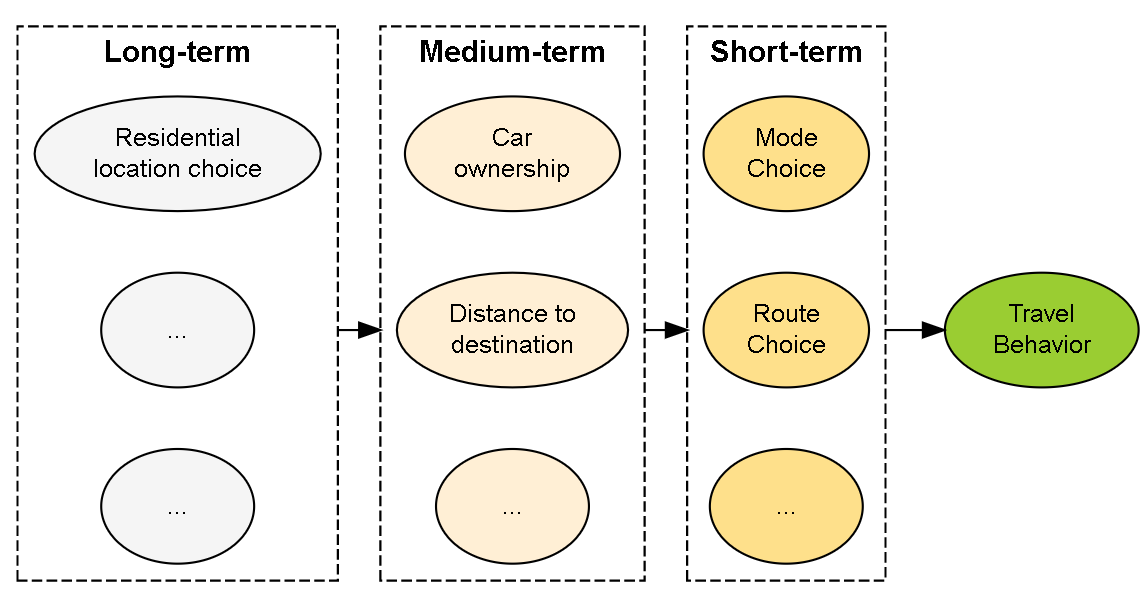
\includegraphics[width=0.5\linewidth]{~/urbanstudy/field_paper/fig/mstage} 

}

\caption{Multistage Structure}\label{fig:Mstage}
\end{figure}

\protect\hyperlink{ref-ben-arivaMETHODOLOGYSHORTRANGETRAVEL1977}{Ben-Ariva and Atherton} (\protect\hyperlink{ref-ben-arivaMETHODOLOGYSHORTRANGETRAVEL1977}{1977}) introduced a hierarchical framework of travel behavior. According to the length of time in travel decision, they divided the relevant factors into three levels. For example, people could change their travel mode choice for each day or each trip. Thus mode choice is a short-term decision
Car ownership belongs medium-term decision since people usually don't purchase or sell a car very often.
Residential location choice is long-term decision because relocation is the most infrequent event than others.

Under this framework, the decisions in longer term can affect the decisions in shorter term, but not vice versa. (Figure \ref{fig:Mstage})
For example, the distance to destination is decided by residential location choice and working location choice. And the distance is also a fundamental factor that influences travel mode choice behavior (\protect\hyperlink{ref-munshiBuiltEnvironmentMode2016}{Munshi 2016}).
In this way, both household car ownership, travel distance and travel attitudes are treated as intermediate variables connecting between built environment and mode choice in decision models. (\protect\hyperlink{ref-dingExploringInfluenceBuilt2017}{Ding, Wang, et al. 2017}; \protect\hyperlink{ref-devosIndirectEffectBuilt2021}{De Vos et al. 2021}).
A VMT models with stepwise framework is as follow.

\begin{equation}
\label{eq:stepwise}
\mathrm{Y}=\mathbf{X}_\mathrm{L}\boldsymbol{\beta}_\mathrm{L}+\mathrm{X_{M}}{\beta}_\mathrm{M}+\mathbf{X}_\mathrm{S}\boldsymbol{\beta}_\mathrm{S}+\boldsymbol{\varepsilon}
\end{equation}

where \(\boldsymbol{\beta}\) are the coefficients with respect to long-term factors \(\mathbf{X}_\mathrm{L}\), medium-term \(\mathrm{X_{M}}\), and short-term covariates \(\mathbf{X}_\mathrm{S}\).
There could be two-way interaction effect between long-term and medium-term variables; three-way interaction effects among long-term, medium-term and short-term variables in the model (Equation \eqref{eq:stepwise}).

This framework works well for commuting trips because people will not change work place very often. The mobility theories also agree with this pattern.
``commuting trips are stable in time and account for the largest fraction of the total flows in a population.'' (\protect\hyperlink{ref-vanackerCommutingTripsTours2011}{Van Acker and Witlox 2011}).

However, the number of non-commuting trips in the U.S. have been more than commuting trips in recent years (TODO source).
For non-commuting travel purposes, such as shopping, leisure, or socializing, the destination choices are more flexible.

The decision could be one-step. In consideration of all the benefit and cost, The traveler make a decision including the destination, mode and route at the same moment.
It also could be multistep. Starting from a travel demand or purpose, the traveler decides to make a trip then choose the destination, mode, route, and departure time step-by-step from available alternatives based on benefit, cost, and habit.
This process is progressive, iterative, and habitual in real life. Hence, the travel distance could be decided before or after mode or route choices. One structure only can capture one aspect of the process.
The framework selection should suit the research question.

\hypertarget{decision-tree}{%
\section{Decision Tree}\label{decision-tree}}

\begin{figure}

{\centering 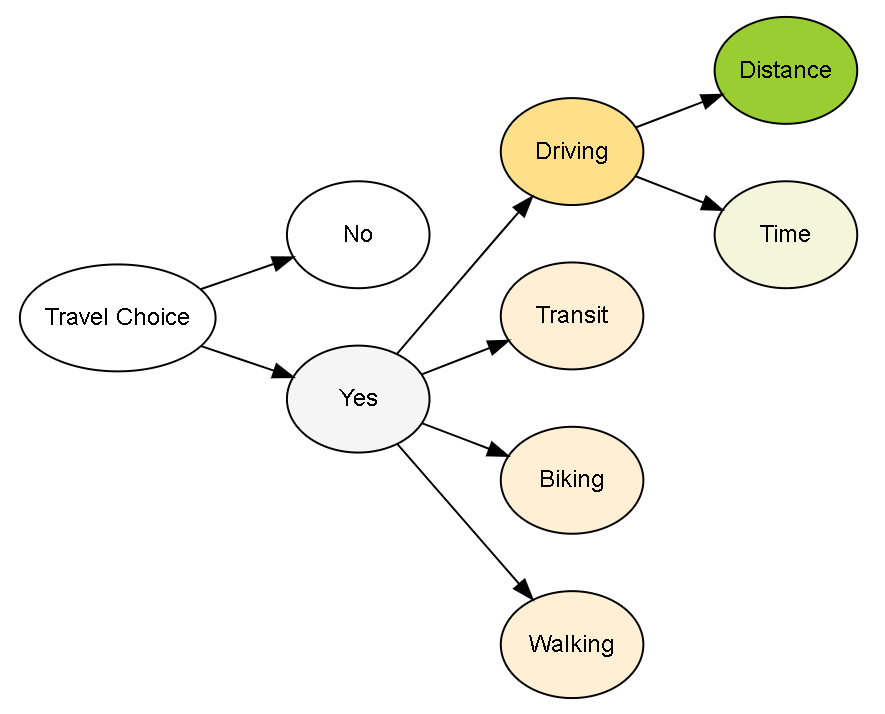
\includegraphics[width=0.5\linewidth]{~/urbanstudy/field_paper/fig/tree} 

}

\caption{Decision Tree Structure}\label{fig:Tree}
\end{figure}

The single-step decision frameworks often require some strong assumptions. For example, the principle of utility maximization applied in either mode choice or VMT models is supposed to explain all the observations, including no-trip or no-driving cases.
Here these observation are treated as censored data with negative utilities. (That will leads to Tobit model for VMT.)

In contrast, a Decision Tree structure allows to use a hierarchical structure to fit different observation respectively (Figure \ref{fig:Tree}).
The model will split into three equations \eqref{eq:Tree}
Starting from a travel demand or purpose, the traveler decides to make a trip or not at the first-level dichotomous node.
A logit or probit model will fit all the data using a suitable model specification.

Then the second layer with polychotomous nodes is about mode choice, which is respect to the multinomial models.
At the bottom layer, a linear (or log-linear) model will only fit the data with positive driving distance (hurdle models; \protect\hyperlink{ref-maModelingTrafficCrash2015}{Ma, Yan, and Weng} (\protect\hyperlink{ref-maModelingTrafficCrash2015}{2015}); \protect\hyperlink{ref-ewingVaryingInfluencesBuilt2015}{Ewing et al.} (\protect\hyperlink{ref-ewingVaryingInfluencesBuilt2015}{2015})).
It is remarkable that the covariates set could vary in different layer's models. For example the lifecycle factor could strongly affect the travel frequency but not affect the driving distance significantly.
Therefore, this structure is more flexible and is consistent with real decision process.

\begin{equation}
\begin{split}
E[\mathbf{Y}_{\{yes,no\}}|\mathbf{X_0}]=&\boldsymbol{\mu_0}=g^{-1}(\mathbf{X_0}\boldsymbol{\beta})\\
E[\mathbf{Y}_{\{car,bus,...\}}|\mathbf{X_1},\mathbf{Y}_{\{yes\}}]=&\boldsymbol{\mu_1}=g^{-1}(\mathbf{X_1}\boldsymbol{\gamma})\\
\mathbf{Z}_{\{car\}}=&\mathbf{X}_\mathrm{2}\boldsymbol{\delta} + \boldsymbol{\varepsilon}
\end{split}
\label{eq:Tree}
\end{equation}

where \(\mathbf{Y}_{\{yes,no\}}\) is a binary variable of making a trip or not. \(\mathbf{Y}_{\{car,bus,...\}}\) is a categorical variable only including the cases of making a trip. \(\mathbf{Z}_{\{car\}}\) is a continuous variable represent driving distance among the group of choosing driving. \(\mathbf{X}_{\{0,1,2\}}\) means the three equations could have different model specifications and will estimate corresponding coefficients, \(\boldsymbol{\beta}\), \(\boldsymbol{\gamma}\), and \(\boldsymbol{\delta}\).

\hypertarget{multi-scales}{%
\section{Multi-scales}\label{multi-scales}}

\begin{figure}

{\centering 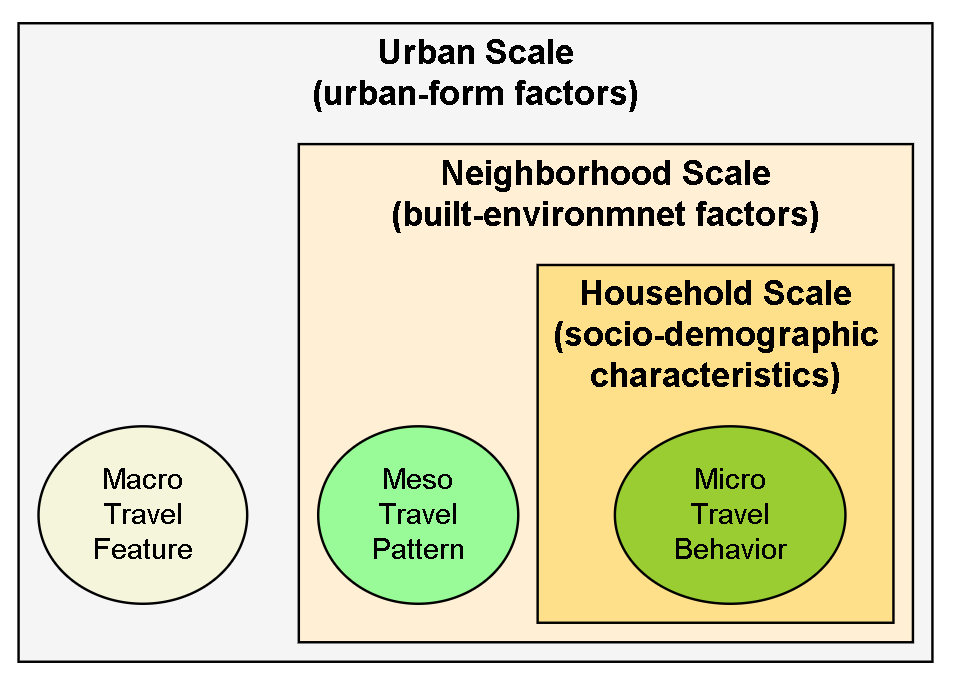
\includegraphics[width=0.5\linewidth]{~/urbanstudy/field_paper/fig/mscale} 

}

\caption{Multi-scales Structure}\label{fig:Mscale}
\end{figure}

As discussed in previous section, the external factors affect individual's travel behavior at multiple scales (Figure \ref{fig:Mscale}).
Van Dender and Clever (2013) doubt weither VMT is determined by local built envrionment factors.

It is necessary to distinguish the meso-scale and macro-scale variable.
The external factors always affect a group of individuals. Therefore, the meso-scale factors like built environment still can be examined. But the social and nature environment will impact all the people living inside the cities and regions.
Only when the data sources cover many cities or regions, these factors can be involved in the models.(Equation \eqref{eq:multiscale})

\begin{equation}
\label{eq:multiscale}
\mathbf{Y}=\mathbf{X}_\mathrm{U}\boldsymbol{\beta}_\mathrm{U}+\mathbf{X}_\mathrm{N}{\beta}_\mathrm{N}+\mathbf{X}_\mathrm{H}{\beta}_\mathrm{H}+\cdots+\boldsymbol{\varepsilon}
\end{equation}

where \(\mathbf{X}_\mathrm{U}\), \(\mathbf{X}_\mathrm{N}\), and \(\mathbf{X}_\mathrm{H}\) are the covariates at the scales of urban, neighborhood, and household. And \(\boldsymbol{\beta}_\mathrm{U}\), \(\boldsymbol{\beta}_\mathrm{N}\), and \(\boldsymbol{\beta}_\mathrm{H}\) are corresponding coefficients respectively.

\hypertarget{other-structures}{%
\section{Other Structures}\label{other-structures}}

\begin{itemize}
\tightlist
\item
  Mixed Model
\end{itemize}

Regression models usually assume the fixed effects of covariate on response. In many cases, some variables should be assigned with random effects.
In travel survey data, every observation are nested in some geographic units, such as tract, TAZ, or city (\protect\hyperlink{ref-dingInfluencesBuiltEnvironment2017}{Ding, Mishra, et al. 2017}).
The geographic location often have some nature of artificial feature influencing travel but the factor is unknown or unobserved.
When the data across many different regions, the model need to control the location effect to identify the crossed effect of built environment. For example, the hypothesis is whether density variable has a strong effects on travel in all place.

In spatial analysis, autocorrelation is a common issue which means the observation values in a location will be affected by its neighbors. Mixed model can help to eliminate the neighborhood effects.

\begin{equation}
\label{eq:multiscale}
\mathbf{Y}=\mathbf{X}_\mathrm{H}\boldsymbol{\beta}+\mathbf{X}_\mathrm{N}{\gamma}+\mathbf{X}_\mathrm{U}{\delta}+\boldsymbol{\varepsilon}
\end{equation}

where \(\mathbf{X}_\mathrm{U}\), \(\mathbf{X}_\mathrm{N}\), and \(\mathbf{X}_\mathrm{H}\) are the same as above. \(\boldsymbol{\beta}\) is a vector of fixed effects. \(\boldsymbol{\gamma}\) and \(\boldsymbol{\delta}\) are two vectors of random effects at neighborhood and urban scales. Assume that \(\boldsymbol{\gamma}\sim N(\mathbf{0}, \boldsymbol{\Sigma}_\mathrm{N})\) and \(\boldsymbol{\delta}\sim N(\mathbf{0}, \boldsymbol{\Sigma}_\mathrm{U})\). And also assume \(Cov(\boldsymbol{\gamma},\boldsymbol{\delta})=Cov(\boldsymbol{\gamma},\boldsymbol{\varepsilon})=Cov(\boldsymbol{\delta},\boldsymbol{\varepsilon})=\mathbf{0}\).

\begin{itemize}
\tightlist
\item
  Non-linear models
\end{itemize}

As \protect\hyperlink{ref-cliftonGettingHereThere2017}{Clifton} (\protect\hyperlink{ref-cliftonGettingHereThere2017}{2017}) said, built environment-travel studies often assume the linearity holds for the density measures and the travel outcome of interest. In practice, the relationship of trip vesus built environment variables may be non-linear or follow a step function with lower and upper threshold. The shape of the curve is highly informative. Recently, scholars have an increasing interest in the non-parameter methods (\protect\hyperlink{ref-dingNonlinearAssociationsZonal2021}{Ding et al. 2021}). The overall effects of density might be small. But the curve might have a steep rise or sheer drop in some intervals. The inflection points, called effective thresholds, are more attractive and instructional. For example, Using Generalized Additive Model (GAM) (\protect\hyperlink{ref-hastieGeneralizedAdditiveModels1990}{Hastie and Tibshirani 1990}), Ewing's study finds some potential points of encouraging shorter driving. His study recommended the suitable activity density (population and employment size/square mile) should be between 10000-25000 according to a center type (Figure \ref{ewing-gam}).
More and more studies reveal the non-linear relationship between population density and VMT (Cheng, De Vos, Zhao, Yang, \& Witlox, 2020; Ding, Cao, \& Næss, 2018; Hong, 2015).
People can interpret the different trends as trigger effects, ceiling effects, U-shapes, hybrid, or synergy effect.

\begin{figure}

{\centering 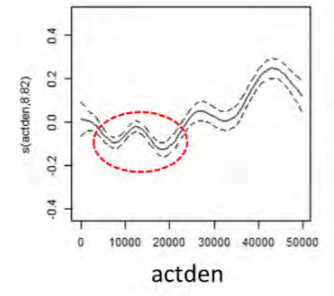
\includegraphics[width=0.5\linewidth]{fig/Ewing_gam1} 

}

\caption{Activity density v.s its smooth function ( Source: Ewing, R. 2021. Webinar: Transportation Benefits of Polycentric Urban Form)}\label{fig:ewing-gam}
\end{figure}

\begin{equation}
\label{eq:nonlinear}
\mathrm{Y}=\mathbf{X}_\mathrm{C}\boldsymbol{\beta}_\mathrm{C}+m(\mathbf{X}_\mathrm{E})\boldsymbol{\beta}_\mathrm{E}+\boldsymbol{\varepsilon}
\end{equation}

In the model (Equation \eqref{eq:nonlinear}), \(m(\mathbf{X}_\mathrm{E})\) is a proper function of built environment covariates.

The non-linear methods can better perform goodness-of-fit, but the generated new data are unique and harder to interpret. The non-linear methods can disclose more information from the data. The risk is that their results are more likely to reflect the features of the data itself and cannot be generalized to other cases.

The results of linear and non-linear models cannot be compared because their underlying assumptions of distribution are different. The threshold studies in urban transportation field remain in the early stages.

\hypertarget{part-part-ii-statistical-methods}{%
\part*{Part II Statistical Methods}\label{part-part-ii-statistical-methods}}
\addcontentsline{toc}{part}{Part II Statistical Methods}

\hypertarget{common-methods}{%
\chapter{Common Methods}\label{common-methods}}

Part II presents some statistical methods relating to Travel-Urban Form models.
Chapter 5 introduce the main methods could be applied on travel-urban form models, including the response variables such as VMT, mode choice, and the frequency of trips.
Chapter 6 lists several potential issues which often be neglected or omitted in travel-urban form models.
The common statistical tools applied in travel-urban form studies are some essential approaches had been developed for decades.
Meanwhile, these principles and algorithms are the premise that further discussions continue.
An overview of new methods in Chapter 7 presents some recent trends in travel-urban form studies that can give some inspiration for future work.
The last chapter Meta-Analysis introduces some basic ideas and approaches of meta-analysis and dealing with publication bias.

\hypertarget{for-travel-distance}{%
\section{For Travel Distance}\label{for-travel-distance}}

\hypertarget{transformations}{%
\subsection{Transformations}\label{transformations}}

Ordinary least squares (OLS) and Multiple Linear Regression (MLR) is the proper method and type of models for continuous response variables. In travel-urban form studies, travel distance belong to this category. Other continuous variables, such as travel time, CO\(_2\) emission are also usual research interests in transportation.

However, These variables have a common feature that their domain is positive number, not whole real number field. Here may raise a debate of whether zero values are a part of these variables or not.
As discussed in previous chapter, the logarithm transformation on these variables can convert the positive values to real numbers, and the zero values are excluded automatically.
Log transformation can also address the issues of linearity and normality.
Log models on travel distance is widely used in transportation related research and practice. A resent example is that Alam et al.~(2018) use log-log model for travel demand by transit at MSA level in U.S.
Here gives two functions of log transform from mathematical perspective: variance stabilizing and linearizing.

\hypertarget{variance-stabilizing}{%
\subsubsection{Variance Stabilizing}\label{variance-stabilizing}}

Equality of variance is a primary assumption of the regression model.
When variance is not constant, the least-squares estimators will not give the minimized variance.
Though the estimation is still unbiased, the standard errors of regression coefficients will be larger and the model becomes insensitive.
\protect\hyperlink{ref-montgomeryIntroductionLinearRegression2021}{Montgomery, Peck, and Vining} (\protect\hyperlink{ref-montgomeryIntroductionLinearRegression2021}{2021}) give several useful variance stabilizing transformations in Table \ref{tab:transformation}.

\begin{table}

\caption{\label{tab:transformation}variance stabilizing transformations}
\centering
\fontsize{7}{9}\selectfont
\begin{tabular}[t]{ll}
\toprule
Relationship & Transformation\\
\midrule
$\sigma^2\propto E[y]$ & $y^{1/2}$\\
$\sigma^2\propto (E[y])^2$ & $\ln(y)$\\
$\sigma^2\propto (E[y])^3$ & $y^{-1/2}$\\
$\sigma^2\propto (E[y])^4$ & $y^{-1}$\\
\bottomrule
\end{tabular}
\end{table}

A preliminary study using National Household Travel Survey (NHTS) (\protect\hyperlink{ref-nhts_2009}{U.S. Department of Transportation, Federal Highway Administration 2009}) data finds both the mean and standard deviation of household daily VMT are close to 40.
This relationship supports that the logarithm of \(\mathbf{y}\) is a proper choice for variance stabilizing.

\hypertarget{linearizing}{%
\subsubsection{Linearizing}\label{linearizing}}

Another fundamental assumption, linearity is also can be addressed by transformation.
If the relationship between response and predictors is linearizable, a suitable transformation can construct a intrinsically linear model.
Several common forms from (\protect\hyperlink{ref-montgomeryIntroductionLinearRegression2021}{Montgomery, Peck, and Vining 2021}) are shown in Table \ref{tab:linearlizing}.

\begin{table}

\caption{\label{tab:linearlizing}Linearizing transformations}
\centering
\fontsize{7}{9}\selectfont
\begin{tabular}[t]{lll}
\toprule
Relationship & Transformation & Linear.Form\\
\midrule
$y=\beta_0\exp[\beta_1x]\varepsilon$ & $y^*=\ln(y),\varepsilon^*=\ln\varepsilon$ & $y^*=\ln \beta_0 +\beta_1x +\varepsilon^*$\\
$y=\beta_0+\beta_1\ln(x)+\varepsilon$ & $x^*=\ln(x)$ & $y=\beta_0 +\beta_1x^*+\varepsilon$\\
$y=\beta_0x^{\beta_1}\varepsilon$ & $y^*=\ln(y),x^*=\ln(x),\varepsilon^*=\ln\varepsilon$ & $y^*=\ln\beta_0 +\beta_1x^* +\varepsilon^*$\\
$y=x/((\beta_0+\varepsilon)x+\beta_1)$ & $y^*=1/y,x^*=1/x$ & $y^*=\beta_0 +\beta_1x^* +\varepsilon$\\
\bottomrule
\end{tabular}
\end{table}

Comparing these forms, the \(log(y)\) transformation also called log-linear model gives a finite value of response \(y\) when predictor \(x\to 0\).
While the log-log model (\(y'=\ln(y),x'=\ln(x)\)) will give an infinite value of \(y\) when \(x\to 0\).
This gives a useful hint when one chooses from log-linear and log-log models.

Moreover, the \(log(y)\) transformation changes the scale of error term.
Only one term in \(\varepsilon\) and \(\ln\varepsilon\) can be close to constant mean and normal distributed.
Therefore, residual diagnosis is still a effective way for choosing the proper form of transformation.
Prior theories and experience can also help to make a proper choice.
Recall the Equation \eqref{eq:gravity-law}, both Gravity law and Zipf's law imply that a logarithm transformation on VMT is suitable.

But in literature, some regression models take logarithm transforms on all variables (\protect\hyperlink{ref-alamFactorsAffectingTravel2018}{\textbf{alamFactorsAffectingTravel2018?}}; \protect\hyperlink{ref-leeComparingImpactsLocal2020}{S. Lee and Lee 2020}), some only transform one or a part of variables (\protect\hyperlink{ref-perumalContextualDensityUS2017}{Perumal and Timmons 2017}), while some models keep the original metrics of data (\protect\hyperlink{ref-zhouSelfSelectionHomeChoice2008}{Zhou and Kockelman 2008}).
Which one is the proper way?
Many of studies don't explain their choice and treat log transform likes a `tradition.'
This question should be answered by checking model adequacy, which is presented in next chapter.
Obviously, the models with and without log transform have different structures and are not equivalent.
Assuming the choice of the two types of model is based on their data and adequacy, the next question is, do their outcomes are comparable?
This question needs further investigation.
If the answer is no, the relevant meta-analysis or summaries should tread them separately.

\hypertarget{estimations}{%
\subsection{Estimations}\label{estimations}}

\begin{itemize}
\tightlist
\item
  Coefficients
\end{itemize}

Estimating the effect size of built environment factors on travel is one of the major goals of travel-urban form studies.
In regression analysis, the values of coefficients represent the effect size.
Least Squares is the mainstream method in the past decades. By \emph{Gauss - Markov theorem}, OLS method itself doesn't require explanatory variables and response variable following normal distribution. If the residuals \(\varepsilon\) satisfy \(E(\varepsilon) = 0\) and \(Var(\varepsilon) = \sigma^2\), the least-squares method will give the unbiased estimators with minimum variance.

Ordinary Least Squares (OLS) method can be used to estimate the coefficients \(\boldsymbol{\beta}\) in equation \eqref{eq:lm} The dimension of \(\mathbf{X}\) is \(n\times p\), which means the data contain \(n\) observations and \(p-1\) predictors. The \(p\times1\) vector of least-squares estimators is denoted as \(\hat\beta\) and the solution to the normal equations is

\begin{equation}
\boldsymbol{\hat\beta}=(\mathbf{X'X})^{-1}\mathbf{X'}\mathbf{y}
\label{eq:lsq-e}
\end{equation}

and

\begin{equation}
\hat\sigma^2=\frac1{n-p}(\mathbf{y-X}\boldsymbol{\hat\beta})'(\mathbf{y-X}\boldsymbol{\hat\beta})
\label{eq:lsq-v}
\end{equation}

Here requires \(\mathbf{X'X}\) are invertible, that is, the covariates are linearly independent if \(\mathbf{X}\) has rank \(p\) (\protect\hyperlink{ref-kimLectureNotes2020}{Kim 2020}, V., Definition, p.22).
When the observations are not independent or have unequal variances, the covariance matrix of error is not identity matrix. The assumption of regression model \(V[\boldsymbol{\varepsilon}]=\sigma^2\mathbf{I}\) doesn't hold. Denote \(\mathbf{V}\) is a known \(n\times n\) positive definite matrix and \(V[\boldsymbol{\varepsilon}]=\sigma^2\mathbf{V}\).
Then, there exists an \(n\times n\) symmetric matrix \(\mathbf{K}\) with rank \(n\) and \(\mathbf{V}=\mathbf{KK'}\). Let

\begin{equation}
\mathbf{z}=\mathbf{K'y},\ \mathbf{B}=\mathbf{K^{-1}X}, \text{and}\ \boldsymbol{\eta}=\mathbf{K'}\boldsymbol{\varepsilon}
\end{equation}

The linear model becomes \(\mathbf{z}=\mathbf{B}\boldsymbol{\beta}+\boldsymbol{\eta}\) and \(V[\boldsymbol{\eta}]=\sigma^2\mathbf{I}\).
If the model is full rank, that is \(rank(\mathbf{X})=p\) then \(\mathbf{X'V^{-1}X}\) is invertible
and the generalized least squares solution is

\begin{equation}
\boldsymbol{\hat\beta}_{GLS}=(\mathbf{X'V^{-1}X})^{-1}\mathbf{X'V^{-1}}\mathbf{y}
\label{eq:glsq-e}
\end{equation}

and

\begin{equation}
\hat\sigma^2_{GLS}=\frac1{n-p}(\mathbf{y-X}\boldsymbol{\hat\beta}_{GLS})'\mathbf{V^{-1}}(\mathbf{y-X}\boldsymbol{\hat\beta}_{GLS})
\label{eq:glsq-v}
\end{equation}

When a study contains two or more travel-urban form models, their response is the same or similar. Researcher can assume that the VMT observed in many cities are random sample from a large population. They often compare the models' performance by adding or removing one or a few independent variables. The coefficients from the best fitted model would be recommended.
But the models in cross studies could choose different combinations of covariates \(\mathbf{X}\) having substantial difference or uncertainties.
In other words, the value of \(\hat \beta_j\) means that, given all other coefficients fixed, for each change of one unit in \(x_j\), the average change in the mean of \(Y\).
Since \(\boldsymbol{\hat\beta}\) are linear combinations of the response and covariates (\protect\hyperlink{ref-montgomeryIntroductionLinearRegression2021}{Montgomery, Peck, and Vining 2021}),
these models should not take the consistent estimated coefficients for granted.

\begin{itemize}
\tightlist
\item
  Standardized coefficients
\end{itemize}

It is inevitable that the units of covariates \(\mathbf{X}\) are very different in many studies. One thing can be done is to
standardize the values of coefficients.
Unit normal scaling or unit length scaling can convert \(\hat \beta_j\) to dimensionless regression coefficient, which is called standardized regression coefficients. Let

\begin{equation}
\begin{split}
z_{ij}=&\frac{x_{ij}-\bar x_j}{\sqrt{\sum_{i=1}^{n}(x_{ij}-\bar x_j)^2}}\\
y^{0}_{i}=&\frac{y_{i}-\bar y}{\sqrt{\sum_{i=1}^{n}(y_{i}-\bar y)^2}}
\end{split}
\label{eq:standize}
\end{equation}

\begin{equation}
\begin{split}
\mathbf{\hat b}=&(\mathbf{Z'Z})^{-1}\mathbf{Z'}\mathbf{y^{0}},\ \text{or}\\
\hat b_j= &\hat\beta_j\sqrt{\frac{\sum_{i=1}^{n}(x_{ij}-\bar x_j)^2}{\sum_{i=1}^{n}(y_{i}-\bar y)^2}},\ j=1,2,...(p-1),\text{ and}\\
\hat\beta_0=&\bar y - \sum_{j=1}^{p-1}\hat\beta_j\bar x_j
\end{split}
\label{eq:stand-coef}
\end{equation}

Note that \(\mathbf{Z'Z}\) correlations matrix.

\begin{equation}
\mathbf{Z'Z}=\begin{bmatrix} 
1 & r_{12} & r_{13} & \dots & r_{1k} \\  
r_{21} & 1 & r_{23} & \dots & r_{2k} \\  
r_{31} & _{32} & 1 & \dots & r_{3k} \\  
\vdots & \vdots & \vdots & \ddots & \vdots \\  
r_{k1} & r_{k2} & _{k3} & \dots & 1  \end{bmatrix},\quad 
\mathbf{Z'}\mathbf{y^{0}}=\begin{bmatrix} 
r_{1y} \\ r_{2y} \\ r_{3y} \\ \vdots \\ r_{ky} \end{bmatrix}
\label{eq:corr-matrix}
\end{equation}

where

\begin{equation}
\begin{split}
r_{ij}=&\frac{\sum_{u=1}^{n}(x_{ui}-\bar x_i)(x_{uj}-\bar x_j)}{\sqrt{\sum_{u=1}^{n}(x_{ui}-\bar x_i)^2\sum_{u=1}^{n}(x_{uj}-\bar x_j)^2}}\\
r_{jy}=&\frac{\sum_{u=1}^{n}(x_{uj}-\bar x_j)(y_{u}-\bar y)}{\sqrt{\sum_{u=1}^{n}(x_{uj}-\bar x_j)^2\sum_{u=1}^{n}(y_{u}-\bar y)^2}}
\end{split}
\label{eq:corr-1}
\end{equation}

Here \(r_{ij}\) is the simple correlation between \(x_i\) and \(x_j\). \(r_{jy}\) is the simple correlation between \(x_j\) and \(y\)

\begin{itemize}
\tightlist
\item
  Elasticity
\end{itemize}

As introduced in previous chapter, elasticity is also commonly used to determine the relative importance of a variable in terms of its influence on a dependent variable. It is generally interpreted as the percent change in the dependent variable induced by a 1\% change in the independent variable (\protect\hyperlink{ref-mccarthyTransportationEconomicsTheory2001}{McCarthy 2001}).

\[e_i=\beta_i\frac{X_i}{Y_i}\approx\frac{\partial Y_i}{\partial X_i}\frac{X_i}{Y_i}\]

\begin{table}

\caption{\label{tab:elas-formula}Elasticity Estimates for Various Functional Forms}
\centering
\fontsize{7}{9}\selectfont
\begin{tabular}[t]{lll}
\toprule
Model & Marginal.Effects & Elasticity\\
\midrule
Linear & $\beta$ & $\beta\frac{X_i}{Y_i}$\\
Log-linear & $\beta Y_i$ & $\beta X_i$\\
Linear-log & $\beta\frac{1}{X_i}$ & $\beta\frac{1}{Y_i}$\\
Log-log & $\beta\frac{Y_i}{X_i}$ & $\beta$\\
Logit & $\beta p_i(1-p_i)$ & $\beta X_i(1-p_i)$\\
\addlinespace
Poisson & $\beta\lambda_{i}$ & $\beta X_i$\\
NB & $\beta \lambda_{i}$ & $\beta X_i$\\
\bottomrule
\end{tabular}
\end{table}

It might be a typo that \protect\hyperlink{ref-ewingTravelBuiltEnvironment2010}{Ewing and Cervero} (\protect\hyperlink{ref-ewingTravelBuiltEnvironment2010}{2010}) use the formula of \(\beta \bar X\left(1-\frac{\bar Y}{n}\right)\) for Logit model.
In Poisson model and Negative Binomial model, \(\lambda_i=\exp[\mathbf{x}_i'\boldsymbol{\beta}]\) (\protect\hyperlink{ref-greeneEconometricAnalysis2018}{\textbf{greeneEconometricAnalysis2018?}}).
For truncated Poisson model: \(\delta_i=\frac{(1-P_{i,0}-\lambda_i P_{i,0})}{(1-P_{i,0})^2}\cdot\lambda_i\beta\) (\protect\hyperlink{ref-greeneEconometricAnalysis2018}{\textbf{greeneEconometricAnalysis2018?}}).
Hurdle model will give separate marginal(partial) effects (\protect\hyperlink{ref-greeneEconometricAnalysis2018}{\textbf{greeneEconometricAnalysis2018?}}, example 18.20).

It seems that standardized regression coefficients are comparable. However, the value of \(\hat b_j\) depends on other predictors. Therefore, comparison between different models is still problematic.
Some studies sums up the standardized coefficients or elasticities and called the summation as combined effects (\protect\hyperlink{ref-leeComparingImpactsLocal2020}{S. Lee and Lee 2020}). Although these values are dimensionless, this method is problematic because different model specifications and data ranges are not comparable.

\hypertarget{inference}{%
\subsection{Inference}\label{inference}}

\hypertarget{analysis-of-variance}{%
\subsubsection{Analysis of Variance}\label{analysis-of-variance}}

Analysis of Variance (ANOVA) is the fundamental approach in regression analysis. Actually, this method analysis the variation in means rather than variances themselves (\protect\hyperlink{ref-casellaStatisticalInference2002}{Casella and Berger 2002, Ch.11}).
Given the estimated coefficients, the model can give the fitted values of response as:

\begin{equation}
\mathbf{\hat y}=\mathbf{X}\boldsymbol{\hat\beta}=\mathbf{X}(\mathbf{X'X})^{-1}\mathbf{X'y}= \mathbf{Hy}
\label{eq:fitted-y}
\end{equation}

where \(\mathbf{H}=\mathbf{X}(\mathbf{X'X})^{-1}\mathbf{X'}\) is hat matrix and \(\mathbf{e}=\mathbf{y}-\mathbf{\hat y}=\mathbf{y}-\mathbf{X}\boldsymbol{\hat\beta}=(\mathbf{I}-\mathbf{H})\mathbf{y}\)

Once the linear relationship holds, the response \(\mathbf{y}\) can be decomposed to

\begin{equation}
\begin{split}
\mathbf{y'y}=&\mathbf{y'Hy}+\mathbf{y'}(\mathbf{I}-\mathbf{H})\mathbf{y}\\
\mathbf{y'y}=&\boldsymbol{\hat\beta}\mathbf{X'}\mathbf{y}+\mathbf{y'y}-\boldsymbol{\hat\beta}\mathbf{X'}\mathbf{y}\\
\mathbf{y'y}-n\bar y^2=&\boldsymbol{\hat\beta}\mathbf{X'}\mathbf{y}-n\bar y^2+\mathbf{y'y}-\boldsymbol{\hat\beta}\mathbf{X'}\mathbf{y}\\
\sum(y-\bar y)^2=&\sum(\hat y-\bar y)^2+\sum(y-\hat y)^2\\
\mathrm{SST} =& \mathrm{SSR} + \mathrm{SSE}
\end{split}
\label{eq:ss}
\end{equation}

where \(\mathrm{SST}\) is Sum of Squares Total, \(\mathrm{SSR}\) is Sum of Squares Regression, and \(\mathrm{SSE}\) is Sum of Square Error. \(\mathrm{SSE}=\mathbf{e'e}\) represents the unknown part of model.

For Generalized Least Squares method, \(\mathrm{SST}=\mathbf{y'V^{-1}y}\), \(\mathrm{SSR}= \boldsymbol{\hat\beta'}\mathbf{B'z}=\mathbf{y'V^{-1}X(X'V^{-1}X})^{-1}\mathbf{X'V^{-1}}\mathbf{y}\), and \(\mathrm{SSE}=\mathrm{SST}-\mathrm{SSR}\)

\hypertarget{hypothesis-test}{%
\subsubsection{Hypothesis Test}\label{hypothesis-test}}

\begin{itemize}
\tightlist
\item
  Significance of Regression
\end{itemize}

Significance of regression means if the linear relationship between response and predictors is adequate. The hypotheses for testing model adequacy are

\begin{equation}
\begin{split}
H_0:&\quad \beta_0 = \beta_1 = \cdots =\beta_{p-1}=0\\
H_1:&\quad \text{at least one } \beta_j \neq 0,\ j=0,1,...,(p-1)\\
\end{split}
\label{eq:hyp-1}
\end{equation}

By Theorem D14 (\protect\hyperlink{ref-kimLectureNotes2020}{Kim 2020},XX, p.90), if an \(n\times1\)random vector \(\mathbf{y}\sim N(\boldsymbol{\mu},\mathbf{I})\), then

\begin{equation}
\mathbf{y'y} \sim \chi^2(n,\frac12\boldsymbol{\mu'\mu})
\label{eq:chisq}
\end{equation}

Recall the assumption of \(\mathbf{y|x}\sim N (\mathbf{X}\boldsymbol{\beta},\sigma^2\mathbf{I})\).\\
By the additive property of \(\chi^2\) distribution,

\begin{equation}
\begin{split}
\frac{MSE}{\sigma^2}=&\frac{\mathbf{y'(I-H)y}}{(n-p)\sigma^2} \sim \chi^2_{(n-p)}\\
\frac{MSR}{\sigma^2}=&\frac{\mathbf{y'Hy}}{(p-1)\sigma^2} \sim \chi^2_{(p-1)}
\end{split}
\label{eq:msemsr}
\end{equation}

Though \(\sigma^2\) is usually unknown, by the relationship between \(\chi^2\) and \(F\) distributions,

\begin{equation}
F_0=\frac{MSE}{MSR} \sim F_{(p-1),(n-p),\lambda}
\end{equation}

where \(\lambda\) is the non-centrality parameter. It allows to test the hypotheses given a significance level \(\alpha\). If test statistic \(F_0>F_{\alpha,(p-1),(n-p)}\), then one can reject \(H_0\).

If a VMT-urban form model added many predictors but adjusted \(R^2\) is still low, the association between travel distance and built environment might be spurious.

\begin{itemize}
\tightlist
\item
  Significance of Coefficients
\end{itemize}

For testing a specific coefficient, the hypothesis is

\begin{equation}
\begin{split}
H_0:&\quad \beta_j =0\\
H_1:&\quad \beta_j \neq 0\\
\end{split}
\label{eq:hyp-2}
\end{equation}

\(\boldsymbol{\hat\beta}\) is a linear combination of \(\mathbf{y}\). Based on the assumption of \(\mathbf{y|x}\sim N (\mathbf{X}\boldsymbol{\beta},\sigma^2\mathbf{I})\), it can be proved that \(\boldsymbol{\hat\beta}\sim N (\boldsymbol{\beta},\sigma^2(\mathbf{X'X})^{-1})\) and

\begin{equation}
t_0=\frac{\hat\beta_j}{se(\hat\beta_j)}=\frac{\hat\beta_j}{\sqrt{\hat\sigma^2C_{jj}}} \sim t_{(n-p)}
\end{equation}

where \(C_{jj}\) is the element at the \(j\) row and \(j\) column of \((\mathbf{X'X})^{-1}\). If \(|t_0|< t_{\alpha/2,(n-p)}\), then the test failed to reject the \(H_0\), this predictor can be removed from the model. This test is called partial or marginal test because the test statistic for \(\beta_j\) depends on all the predictors in the model.

\hypertarget{confidence-intervals}{%
\subsubsection{Confidence Intervals}\label{confidence-intervals}}

Above results can also construct the confidence interval for each coefficient. A \(100(1-\alpha)\) confidence interval for \(\beta_j\) is

\begin{equation}
\hat\beta_j-t_{\alpha/2,(n-p)}\sqrt{\hat\sigma^2C_{jj}}\le \beta_j \le \hat\beta_j+t_{\alpha/2,(n-p)}\sqrt{\hat\sigma^2C_{jj}}
\end{equation}

\pagebreak

\hypertarget{for-tirp-generation}{%
\section{For Tirp Generation}\label{for-tirp-generation}}

ordinal counts Poisson Respone/Loglinear Models

The frequency of trip is count data. The observed trip counts \(Y_i,...,Y_n\) are random variable aggregated over differing numbers of individual or household with support \(Y=\in\{0,1,2,...\}\).
The trips as events occur randomly in a day or other time.
An usual assumption is that count data follow a Poisson distribution.

There are three conditions for Poisson process:
Firstly, as a stochastic process, the probability of at least one event happened in a time interval is proportional to the length of the interval.
secondly, the probability of two or more event happened in a small time interval is close to zero.
Finally, in disjoint time intervals, the count numbers of trip should be independent.
In real life, a traveler can not make two trips at the same time so the second condition holds.
But a household with two worker and two student might have four trip at the same time every morning. Hence, individual count data is more valid than household's when using Poisson distribution.
The independency of count number among differing time interval may not valid too. The daily trips is often a trip chain and require more information at a micro level.

The pmf and its canonical form is

\begin{equation}
Pr(Y=y) = \frac{e^{-\mu}\mu^y}{y!}=\exp[\log(\mu) y-\mu](y!)^{-1}
\end{equation}

So Poisson distribution has a simple link function as

\begin{equation}
\begin{split}
g(\mu_i)&=\log\mu_i=\eta_i\\
g^{-1}(\eta_i)&=\exp[\eta_i]=\mu_i\\
\end{split}
\label{eq:pois-link}
\end{equation}

And Poisson distribution has the property of \(E[y_i]=Var[y_i]=\mu_i\) as the systematic component.

\begin{equation}
\begin{split}
\log(\mu_i)=&\mathbf{x}'\boldsymbol{\beta}\\
\mu_i=&\exp[\mathbf{x}'\boldsymbol{\beta}]\\
\end{split}
\end{equation}

By taking log transform, the non-negative parameter space mapping to real number.
It also convert the multiplicative relationship among predictors to additive.
The value of coefficient \(\beta_j\) means that per unit change in predictor \(x_j\) leads to the expected change in the log of the mean of response.
Another interpretation is that the mean of response would multiple \(\exp[\beta_j]\) by per unit change in \(x_j\).

Similarly, iteratively reweighted least squares method (IRLS) can solve the log-linear Poisson model.
The key correction step is

\begin{equation}
\hat{\eta_i}^{(1)}=\hat{\eta_i}^{(0)} + \frac{y_i-\hat\mu_i^{(0)}}{\hat\mu_i^{(0)}}
\end{equation}

The diagonal weight matrix is

\begin{equation}
w_{ii}=\hat\mu_i^{(0)}
\end{equation}

\hypertarget{negative-binomial-model}{%
\subsection{Negative Binomial Model}\label{negative-binomial-model}}

The restriction of Poisson Distribution is that the mean and variance should be equal or proportional.
In many count data, the inequality of them is called overdispersion.

Suppose an unobserved random variable follow a gamma distribution \(Z\sim Gamma(r,1/r)\) where \(r\) is the shape parameter. The pdf is

\begin{equation}
f(z)=\frac{r^r}{\Gamma(r)}z^{r-1}\exp[-rz],\quad z>0
\end{equation}

It has \(E[Z]=1\) and \(Var[Z]=1/r\).

Then a mixture model can be denote as a conditional distribution \(Y|Z\sim Pois(\mu Z)\) for some \(\mu>0\) and

\begin{equation}
E[Y]=E[E[Y|Z]]=E[\mu Z]=\mu E[Z]=\mu
\end{equation}

and

\begin{equation}
\begin{split}
Var[Y]&=E[Var[Y|Z]] + Var[E[Y|Z]]\\
&=E[\mu Z]+Var[\mu Z]\\
&=\mu E[Z] + \mu^2Var[Z]\\
&=\mu+\frac{\mu^2}{r}
\end{split}
\end{equation}

It is called Poisson-Gamma distribution who can represents the inequality of mean and variance.
If \(r\) represent the given number of success and \(y\) represent the observed number of failure in a sequence of independent Bernoulli trails. Then the success probability is \(p=r/(r+\mu)\)
Recall that \(\Gamma(r+y)=\int_0^\infty z^{r+y-1}\exp[-z]dz\), it can be proved that \(Y\) follow a negative binomial distribution

\begin{equation}
\begin{split}
p(y)&=\int_0^\infty p(y|z)\cdot f(z)dz\\
&=\int_0^\infty \frac{(\mu z)^y\exp[-\mu z]}{y!}\cdot\frac{r^r}{\Gamma(r)}z^{r-1}\exp[-rz]dz\\
&=\frac{r^r\mu^y}{y!\Gamma(r)}(\mu+r)^{-y-r}\int_0^\infty [(\mu+r)z]^{y+r-1}\exp[-(\mu+r)z]d(\mu+r)z\\
&=\frac{\Gamma(r+y-1)}{\Gamma(y+1)\Gamma(r)}(\frac{r}{\mu+r})^r(\frac{\mu}{\mu+r})^y\\
&={{r+y-1}\choose{r-1}}p^r(1-p)^y, \quad y=0,1,2,...
\end{split}
\end{equation}

However, negative binomial distribution is non-exponential families. Using maximum likelihood method and log link, the coefficients can be estimated.

\hypertarget{quasi-poisson-model}{%
\subsection{Quasi-Poisson Model}\label{quasi-poisson-model}}

Another simple way for overdispersion is to introduce a dispersion parameter \(\phi\). The Poisson model has \(Var[Y|\eta]=\phi\mu\) where \(\phi>1\). The estimated \(\phi\) is

\[
\hat\phi=\frac{1}{n-p}\sum\frac{(Y_i-\hat\mu_i)^2}{\hat\mu_i}
\]
The extra parameter can also be estimated by maximum likelihood.

\hypertarget{zero-inflated-and-hurdle-models}{%
\subsection{Zero-inflated and Hurdle Models}\label{zero-inflated-and-hurdle-models}}

In trip frequency data, there are often more no-trip observations than Poisson and negative binomial distribution expected. The two types of models, zero-inflated model and hurdle model can address this issue.
Both of them assume the data arise from two mechanisms.

In Zero-inflated Poisson/negative binomial model, both of two mechanisms generate zero observations.\\
The first mechanism produce the excess zeros with \(\pi_i=Pr(Y_i=0)\). The rest zero and positive values are generated by the second mechanism \(f(y;\mathbf{x}_i,\boldsymbol\beta)\) of Poisson or negative binomial pmfs.

\begin{equation}
f(y_i;\pi_i,\mu_i)=\begin{cases}\pi_i+(1-\pi_i)f(0;\mu_i)&y_i=0\\
(1-\pi_i)f(y_i;\mu_i)&y_i>0\\
\end{cases}
\label{eq:zi}
\end{equation}

The two link functions are

\begin{equation}
\begin{split}
g_0(\pi_i)=&\mathbf{w}'_i\boldsymbol\gamma\\
g_1(\mu_i)=&\mathbf{x}'_i\boldsymbol\beta\\
\end{split}
\end{equation}

Note that the two mechanisms could have different covariates and coefficients.
But both of \(\pi_i\) and \(\mu_i\) appear in two equations and have to be evaluated jointly. Newton-Raphson algorithm or EM algorithm can deal with this question.

Hurdle model assumes all zero observations are generated by the first mechanism. Hence the first mechanism is not depend on \(\mathbf{x}_i\) and \(\boldsymbol\beta\).
A challenge is that ordinary Poisson or negative binomial distribution does contain zero values. Here use a truncated distribution to address this issue.

\begin{equation}
f(y_i;\pi_i,\mu_i)=\begin{cases}\pi_i&y_i=0\\
(1-\pi_i)\frac{f(y;\mu_i)}{1-f(0;\mu_i)}&y_i>0\\
\end{cases}
\label{eq:hurdle}
\end{equation}

where \(f(0;\mu_i)= \exp[-\mu_i]\) in Poisson model and \(f(0;\mu_i)= (\frac{r}{\mu_i+r})^r\) in negativ binomial model.

``When \(\pi\) is close to 0 or close to 1, the standard error is artificially compressed, which leads us to overestimate the precision of the proportion estimate.'' (Lipsey and Wilson 2001, chap.~3)

\hypertarget{for-mode-choice}{%
\section{For Mode Choice}\label{for-mode-choice}}

Generalized Linear Models (GlM) allow the response following more general distributions than normal.
It is very important for the research with discrete response variables, such as mode choice or trips counts.

GLM (equation \eqref{eq:glm}) include three components.
Systematic component \(\eta=\mathbf{X}\boldsymbol\beta\) has a similar form with ordinary linear models but without error term. \(\boldsymbol\beta\) are unknown coefficients.
Random component \(E[Y]=\mu\) specifies the probability distributions of \(Y\), which could have a pdf or pmf from an exponential family.
Link function \(g(\cdot)\) connects the systematic component and random component together.

\hypertarget{logit-models}{%
\subsection{Logit Models}\label{logit-models}}

Binomial Response Models

When a traveler choose to make a trip or not, the decision follows a Bernoulli distribution. Denotes the probability \(Pr(\text{choice}=\text{Yes})=\pi\) and \(Pr(\text{choice}=\text{No})=1-\pi\).
For \(n\) number of decisions under the same \(\pi\), let \(Y\) represents the count of choosing `Yes' and follow a binomial distribution \(Bin(n,\pi)\).
For many travelers with different \(\pi\), one has \(Y_i\sim Bin(n_i,\pi_i)\), that is a binary response data. The number of total observation \(N=\sum_{i=1}^n n_i\). The pmf of binomial distribution is

\begin{equation}
Pr(Y_i = y_i) =  {{n_i}\choose{y_i}}  \pi_i^{y_i} (1-\pi_i)^{n_i-y_i}
\end{equation}

It is clear that the random component is \(E[y_i]=\pi_i\) and systematic component \(\eta_i=\mathbf{X}'_i\boldsymbol\beta\).
\(\pi\) is the probability between zero and one. but the log odds of success \(\eta_i\) can take any real number. The canonical form of binomial distribution is

\begin{equation}
Pr(Y_i = y_i) = \exp\left[\log(\frac{\pi_i}{1-\pi_i})y_i+n_i\log(1-\pi_i)\right]{{n_i}\choose{y_i}}
\end{equation}

The canonical link function in logit models can transform the probability to the range of real number. In this one-to-one mapping, a probability \(\pi_i>1/2\) will give a positive \(\eta_i\) and a negative \(\eta_i\) correspond to a \(\pi_i\) less than one half.

\begin{equation}
\begin{split}
g(\pi_i)&=\log\frac{\pi_i}{1-\pi_i}=\eta_i\quad\text{Logit function}\\
g^{-1}(\eta_i)&=\frac{\exp[\eta_i]}{1+\exp[\eta_i]}=\pi_i\quad\text{Logistic function}\\
\end{split}
\label{eq:logit-link}
\end{equation}

The goal is to estimate the unknown vector of parameters \(\boldsymbol\beta\) for the known covariates \(\mathbf{X}_i\).
But in the systematic component, \(\eta_i\) is unobserved. Ordinary Linear Regression doesn't work in this case.
Fortunately, the link function in logit models has a close form.
Iteratively Reweighted Least Squares method (IRLS) (Lawson 1961) can get the solution.
One iteration of this approach includes four steps.

The first step starts from the current estimated coefficients \(\boldsymbol{\hat\beta}^{(0)}\). Then the current estimates of \(\hat{\eta_i}^{(0)}=\mathbf{x}_i'\boldsymbol{\hat\beta}^{(0)}\) and \(\hat \pi_i^{(0)}=\frac{\exp[\hat\eta_i^{(0)}]}{1+\exp[\hat\eta_i^{(0)}]}\).
But current \(\hat{\eta_i}^{(0)}\) is different with the true \(\eta_i\).

The second step will update the current estimates by adding a correction term.
Using the first two terms of Taylor series,

\begin{equation}
\hat{\eta_i}^{(1)}=\hat{\eta_i}^{(0)} +(y_i-\hat\mu_i^{(0)})\cdot \frac{d\hat\eta_i^{(0)}}{d\hat\mu_i^{(0)}}
\end{equation}

Since \(E[Y_i]=\mu_i=n_i\pi_i\), it is also easy to get

\begin{equation}
\frac{d \eta_i}{d \mu_i}=\frac{1}{n_i}\cdot\frac{d \eta_i}{d \pi_i}=\frac{1}{n_i}\left(\frac{1}{\pi_i}+\frac{1}{1-\pi_i}\right)=\frac1{n_i\pi_i(1-\pi_i)}
\end{equation}
Therefore,
\begin{equation}
\hat{\eta_i}^{(1)}=\hat{\eta_i}^{(0)} + \frac{y_i-n_i\hat\pi_i^{(0)}}{n_i\hat\pi_i^{(0)}(1-\hat\pi_i^{(0)})}
\end{equation}

The third step is to calculate the diagonal weight matrix \(\mathbf{W}\) in the Fisher scoring algorithm.
It is known that the binomial distribution has \(Var[Y_i]=n_i\pi_i(1-\pi_i)\).

\begin{equation}
w_{ii}=\left[Var[Y_i](\frac{d \eta_i}{d \mu_i})^2\right]^{-1}=
n_i\hat\pi_i(1-\hat\pi_i)
\end{equation}

The final step improves estimate of \(\boldsymbol{\hat\beta}^{(1)}\) using the weighted least-squares method

\begin{equation}
\hat{\boldsymbol{\beta}}^{(1)}=\mathbf{(X'WX)^{-1}}\mathbf{X'W}\boldsymbol{\hat{\eta}}^{(1)}
\end{equation}

The four steps will repeat until the procedure convergence. And the result gives

\begin{equation}
Var[\hat{\boldsymbol{\beta}}]=\mathbf{(X'WX)^{-1}}
\end{equation}

\hypertarget{multinomial-logit-models}{%
\subsection{Multinomial Logit models}\label{multinomial-logit-models}}

Multinomial Response Models

For categorical response such as travel mode choice, a traveler has more than two alternatives including driving, transit, biking and walking. The generalized logistic regression can address these polychotomous data.

The mode choice \(Y_i\) follows the mutinomial distribution with \(J\) alternatives.
Denote the probability of \(i\)th traveler chooses the \(j\)th mode, then

\begin{equation}
\pi_{ij}=Pr(Y_i=j)
\end{equation}

And the pmf of multinomial distribution is

\begin{equation}
Pr(Y_{i1}=y_{i1}, ..., Y_{iJ}=y_{iJ})= {n_i \choose y_{i1},..., y_{iJ} }
\pi_{i1}^{y_{i1}} \cdots \pi_{iJ}^{y_{iJ}}
\end{equation}

When the data exclude the people without trip, the several modes exhaust all observations and mutually exclusive. That is \(\sum_{j=1}^J\pi_{ij}=1\) for each \(i\). Once \(J-1\) parameters are evaluated, the rest one will be determined automatically. That means \(\pi_{iJ}=1-\pi_{i1}-\cdots-\pi_{i,J-1}\).
The random component is \(\mu_i=n_i\pi_{ij}\)

\begin{equation}
\begin{split}
g^{-1}(\eta_{ij})&=\frac{\exp[\eta_{ij}]}{\sum_{k=1}^J\exp[\eta_{ik}]}=\pi_{ij}\\
g(\pi_{ij})&=\log\frac{\pi_{ij}}{\pi_{iJ}}=\eta_{ij}\\
\end{split}
\label{eq:mlogit-link}
\end{equation}

And the systematic component is \(\eta_{ij}=\mathbf{X}_i'\boldsymbol\beta_j\)

\hypertarget{discret-choice-models}{%
\subsection{Discret Choice Models}\label{discret-choice-models}}

\protect\hyperlink{ref-mcfaddenConditionalLogitAnalysis1973}{McFadden} (\protect\hyperlink{ref-mcfaddenConditionalLogitAnalysis1973}{1973}) proposed the discrete choice models also called multinomial/conditional logit model.
This model introduces \(U_{ij}\) as the random utility of \(j\)th choice. Then based on Utility Maximum theory,

\begin{equation}
\pi_{ij}=Pr(Y_i=j)=Pr(\max(U_{i1},...,U_{iJ})=U_{ij})
\end{equation}

Here \(U_{ij}=\eta_{ij}+\varepsilon_{ij}\) where the error term follows a standard Type I extreme value distributions. The reason is that the difference between two independent extreme value distributions has a logistic distribution. Hence, it can still be solved by logit models.

The expected utility depend on the characteristics of the alternatives rather than that of individuals.
Let \(\mathbf{Z}_j\) represents the characteristics of \(j\)th alternative, one has \(\eta_{ij}=\mathbf{Z}_i'\boldsymbol\gamma\).

Combining the two sources of utility together, a general form of utility is

\begin{equation}
\eta_{ij}=\mathbf{X}_i'\boldsymbol\beta_j+\mathbf{Z}_i'\boldsymbol\gamma
\end{equation}

In reality, a travel data can try to keep the observations independently by random sampling.
But the available travel modes are not independent.
The multinomial/conditional probit model can deal with this issue better.
If assume the error terms \(\boldsymbol\varepsilon\sim MVN(\mathbf{0},\Sigma)\) where \(\Sigma\) is a correlation matrix.

\hypertarget{several-issues}{%
\chapter{Several Issues}\label{several-issues}}

\hypertarget{assumptions}{%
\section{Assumptions}\label{assumptions}}

\hypertarget{additive-and-linearity}{%
\subsection{Additive and linearity}\label{additive-and-linearity}}

For linear models, the most important assumptions are the additive and linear relationship between the response and predictors. Gravity Law discloses that travel distance has a multiplicative (inverse) relationship with the `masses' of two places. If the population size can be a representative of built environment, the additive relationship will not hold. Previous studies also shows that the effect sizes of built environment with respect of travel are small and complex. There is not sufficient evidence to support or against the linear hypothesis.

\hypertarget{independent-identically-distributed-iid}{%
\subsection{Independent Identically Distributed (IID)}\label{independent-identically-distributed-iid}}

Another essential assumption is that random error are Independent Identically Distributed (IID). Random error is also called residual, which refer to the difference between observed \(\mathbf{y}\) and fitted \(\mathbf{\hat y}\). \(\mathbf{\hat y}\) are the linear combinations of predictors \(\mathbf{X}\). residuals represent the part can not be explained by the model.

\begin{equation}
\mathbf{e}=\mathbf{y}-\mathbf{\hat y}
\label{eq:residual}
\end{equation}

The expected value, the variances, and the covariances among the random errors are the first- and second-moment of residuals. `Identical' means that random errors should have zero mean and constant variance. The homogeneity of variance is also called homoscedasticity.

\begin{equation}
E(\varepsilon) = 0, \quad Var(\varepsilon) = \sigma^2
\label{eq:identical}
\end{equation}

`Independent' requires the random errors are uncorrelated. That is

\begin{equation}
Cov[\varepsilon_i,\varepsilon_j] = 0,\quad i\neq j
\label{eq:indenpendent}
\end{equation}

Once the conditions of IID are satisfied, the Gauss - Markov theorem proves that least-square method could give the minimum-variance unbiased estimators (MVUE) or called the best linear unbiased estimators (BLUE). These conditions are not strict and make regression method widely applicable.

Unfortunately, many of the predictors are correlated. Moreover, the observations from various cities, regions, or counties are very unlikely identical. This issue is called heteroscedasticity. Related contents are in Section of Adequacy.

\hypertarget{normality}{%
\subsection{Normality}\label{normality}}

When conducting hypothesis test and confidence intervals, the required assumption is \(\mathbf{y|x}\sim N (\mathbf{X}\boldsymbol{\beta},\sigma^2\mathbf{I})\). Maximum Likelihood Methods also requires this assumption.

Evidence has demonstrated that travel distance is not Normal distributed. The Zipf's law also prove that travel distance follows a power distribution. Using logarithm transformations, the skewed distribution can be converted to an approximate normal distribution.

There are some quantitative methods which can examine nomalirty of the transformed distributions.

\hypertarget{adequacy}{%
\section{Adequacy}\label{adequacy}}

The outcome of estimation and inference can not demonstrate model's performance.
If the primary assumptions is violated, the estimations could be biased and the model could be useless. These problems can also happen when the model is not correctly specified. It is necessary to make diagnosis and validation for fitted models.

\hypertarget{goodness-of-fit}{%
\subsection{Goodness of fit}\label{goodness-of-fit}}

This structure tell us how good the model can explain the data. Coefficient of Determination \(R^2\) is a proportion to assess the quality of fitted model.

\begin{equation}
R^2 =\frac{SSR}{SST}=1-\frac{SSE}{SST}
\label{eq:rsq}
\end{equation}

when \(R^2\) is close to \(1\), the most of variation in response can be explained by the fitted model. Although \(R^2\) is not the only criteria of a good model, it is often available in most published papers. Recall the discussion in Part I, the aggregated data will eliminate the difference among individuals, households, or neighborhoods. In the new variance structure, \(SSE\) will be much less than disaggregated model. The \(R^2\) in many disaggregate studies are around 0.3, while the \(R^2\) in some aggregate studies can reach 0.8. A seriously underfitting model's outputs could be biased and unstable.

A fact is that adding predictors into the model will never decrease \(R^2\). Thus the models with different number of predictors is not comparable. Adjusted \(R^2\) can address this issue by introducing degree of freedom. The degree of freedom denotes the amount of information required to know.

\begin{equation}
\begin{split}
df_T =& df_R + df_E\\
n-1=&(p-1)+(n-p)
\end{split}
\label{eq:df}
\end{equation}

Then, the mean square (MS) of each sum of squares (SS) can be calculated by \(MS=SS/df\). The mean square error \(MSE\) is also called as the expected value of error variance \(\hat\sigma^2=MSE=SSE/(n-p)\). \(n-p\) is the degree of freedom. Then adjusted \(R^2\) is

\begin{equation}
R_{adj}^2 = 1-\frac{MSE}{MST} = 1-\frac{SSE/(n-p)}{SST/(n-1)}
\label{eq:rsq-adj}
\end{equation}

Another similar method is \(R^2\) for prediction based on PRESS.
Recall the PRESS statistic is the prediction error sum of square by fitting a model with \(n-1\) observations.

\begin{equation}
PRESS = \sum_{i=1}^n(y_i-\hat y_{(i)})^2= \sum_{i=1}^n\left(\frac{e_i}{1-h_{ii}}\right)^2
\label{eq:press}
\end{equation}

A model with smaller PRESS has a better ability of prediction. The \(R^2\) for prediction is

\begin{equation}
R_{pred}^2 = 1-\frac{PRESS}{MST}
\label{eq:rsq-pred}
\end{equation}

\hypertarget{residuals-analysis}{%
\subsection{Residuals Analysis}\label{residuals-analysis}}

The major assumptions, both IID and normality are related to residual.
Residual diagnosis is an essential step for modeling validation.

There are several scaled residuals can help the diagnosis.
Since \(MSE\) is the expected variance of error \(\hat\sigma^2\) and \(E[\varepsilon]=0\), standardized residuals should follow a standard normal distribution.

\[d_i=\frac{e_i}{\sqrt{MSE}}=e_i\sqrt{\frac{n-p}{\sum_{i=1}^n e_i^2}},\quad i=1,2,...,n\]

Recall random error \(\mathbf{e}=\mathbf{y}-\mathbf{\hat y}=(\mathbf{I}-\mathbf{H})\mathbf{y}\) and hat matrix \(\mathbf{H}=\mathbf{X}(\mathbf{X'X})^{-1}\mathbf{X'}\).
Let \(h_{ii}\) denote the \(i^{th}\) diagonal element of hat matrix.
Studentized Residuals can be expressed by
\[r_i=\frac{e_i}{\sqrt{MSE(1-h_{ii})}},\quad i=1,2,...,n\]
It is proved that \(0\le h_{ii}\le1\).
An observation with \(h_{ii}\) closed to one will return a large value of \(r_i\). The \(x_i\) who has strong influence on fitted value is called leverage point.

Ideally, the scaled residual have zero mean and unit variance. Hence, an observation with \(|d_i|>3\) or \(|r_i|>3\) is a potential outlier.

Predicted Residual Error Sum of Squares (PRESS) can also be used to detect outliers.
This method predicts the \(i^{th}\) fitted response by excluding the \(i^{th}\) observation and examine the influence of this point.
The corresponding error \(e_{(i)}=e_{i}/(1-h_{ii})\) and \(V[e_{(i)}]=\sigma^2/(1-h_{ii})\).
Thus, if \(MSE\) is a good estimate of \(\sigma^2\), PRESS residuals is equivalent to Studentized Residuals.

\[\frac{e_{(i)}}{\sqrt{V[e_{(i)}]}}=\frac{e_i/(1-h_{ii})}{\sqrt{\sigma^2/(1-h_{ii})}}=\frac{e_i}{\sqrt{\sigma^2(1-h_{ii})}}\]

\begin{itemize}
\tightlist
\item
  Residual Plot
\end{itemize}

Residual plot shows the pattern of the residuals against fitted \(\mathbf{\hat y}\).
If the assumptions are valid, the shape of points should like a envelope and be evenly distributed around the horizontal line of \(e=0\).

A funnel shape in residual plot shows that the variance of error is a function of \(\hat y\). A suitable transformation to response or predictor could stabilize the variance.
A curved shape means the assumption of linearity is not valid. It implies that adding quadratic terms or higher-order terms might be suitable.

\begin{itemize}
\tightlist
\item
  Normal Probability Plot
\end{itemize}

A histogram of residuals can check the normality assumption.
The highly right-skewed probability distribution of VMT log-transform of VMT is reasonable.

A better way is a normal quantile -- quantile (QQ) plot of the residuals.
An ideal cumulative normal distribution should plot as a straight line.
Only looking at the \(R^2\) and p-values cannot disclose this feature.

\hypertarget{heteroscedasticity}{%
\subsection{Heteroscedasticity}\label{heteroscedasticity}}

When the assumption of constant variance is violated, the linear model is heteroscedastic.
Heteroscedasticity is common in urban studies. For example, the cities with different size are not identical. Small cities or rural areas might have homogeneous values of population density, while large cities' densities are more variable.

Recall Generalized least square estimates \eqref{eq:glsq-e} and \eqref{eq:glsq-v}, if the residuals are independent but variances are not constant, a simple linear model becomes \(\boldsymbol{\varepsilon}\sim MVN(\mathbf{0},\sigma^2\mathbf{V})\) where

\begin{equation}
\mathbf{V}=\begin{bmatrix} 
x_1^2 & 0 & \dots & 0 \\  
0 & x_2^2 & \dots & 0 \\  
\vdots & \vdots & \ddots & \vdots \\  
0 & 0 & \dots & x_n^2 \end{bmatrix},\quad 
\mathbf{V}^{-1}=\begin{bmatrix} 
\frac1{x_1^2} & 0 & \dots & 0 \\  
0 & \frac1{x_2^2} & \dots & 0 \\  
\vdots & \vdots & \ddots & \vdots \\  
0 & 0 & \dots & \frac1{x_n^2} \end{bmatrix}
\label{eq:hete-matrix}
\end{equation}

Then \(\mathbf{X'V^{-1}X}=n\) and the generalized least squares solution is

\begin{equation}
\hat\beta_{1,WLS}=\frac1n\sum_{i=1}^{n}\frac{y_i}{x_i}
\label{eq:hete-e}
\end{equation}

and

\begin{equation}
\hat\sigma^2_{WLS}=\frac1{n-1}\sum_{i=1}^{n}\frac{(y_i-\hat\beta_{1}x_i)^2}{x_i^2}
\label{eq:hete-v}
\end{equation}

In heteroscedastic model, the OLS estimates of coefficients are still unbiased but no longer efficient.
But the estimates of variances are biased. The corresponding hypothesis test and confidence interval would be misleading.

Another special case is the model with aggregated variables, which is the cases of geographic unit.
Let \(u_j\) and \(v_j\) are the response and predictors of \(j^{th}\) household in a neighborhood. \(n_i\) is the sample size in each neighborhood. Then \(y_i=\sum_{j=1}^{n_i}u_j/n_i\) and \(X_i=\sum_{j=1}^{n_i}v_j/n_i\). In this case,

\begin{equation}
\mathbf{V}=\begin{bmatrix} 
\frac1{n_1} & 0 & \dots & 0 \\  
0 & \frac1{n_2} & \dots & 0 \\  
\vdots & \vdots & \ddots & \vdots \\  
0 & 0 & \dots & \frac1{n_n} \end{bmatrix},\quad 
\mathbf{V}^{-1}=\begin{bmatrix} 
n_1 & 0 & \dots & 0 \\  
0 & n_2 & \dots & 0 \\  
\vdots & \vdots & \ddots & \vdots \\  
0 & 0 & \dots & n_n \end{bmatrix}
\label{eq:agg-matrix}
\end{equation}

Then \(\mathbf{X'V^{-1}X}=\sum_{i=1}^nn_ix_i^2\) and the WLS estimate of \(\beta_1\) is

\begin{equation}
\hat\beta_{1,WLS}=\frac1n\frac{\sum_{i=1}^{n}n_ix_iy_i}{\sum_{i=1}^{n}n_ix_i^2}
\label{eq:agg-e}
\end{equation}

and

\begin{equation}
V[\hat\beta_{1,WLS}]=\frac{V[\sum_{i=1}^{n}n_ix_iy_i]}{(\sum_{i=1}^{n}n_ix_i^2)^2}=\frac{\sum_{i=1}^{n}n_i^2x_i^2\sigma^2/n_i}{(\sum_{i=1}^{n}n_ix_i^2)^2}=\frac{\sigma^2}{\sum_{i=1}^{n}n_ix_i^2}
\label{eq:agg-v}
\end{equation}

There are three procedures, Bartlett's likelihood ratio test, Goldfeld-Quandt test, or Breusch-Pagan test which can be used to examine heteroscedasticity (\protect\hyperlink{ref-ravishankerFirstCourseLinear2020}{Ravishanker and Dey 2020, 8.1.3, pp.288--290})

\hypertarget{autocorrelation}{%
\subsection{Autocorrelation}\label{autocorrelation}}

For spatio-temporal data, the observations often have some relationship over time or space.
In these cases, the assumption of independent errors is violated, the linear model with serially correlated errors is called autocorrelation.
Autocorrelation is also common in urban studies. All the neighboring geographic entities or stages could impact each other, or sharing the similar environment.

Take a special case of time-series data for example, assuming the model have constant variance. \(E[\varepsilon]=0\) but \(Cov[\varepsilon_i,\varepsilon_j]=\sigma^2\rho^{|j-i|}\), \(i,j=1,2,...,n\) and \(|\rho|<1\)
The variance-covariance matrix is also called Toeplitz matrix as below

\begin{equation}
\mathbf{V}=\begin{bmatrix} 
1 & \rho & \rho^2 & \dots & \rho^{n-1} \\  
\rho & 1 & \rho & \dots & \rho^{n-2} \\  
\vdots & \vdots & \vdots & \ddots & \vdots \\  
\rho^{n-1} & \rho^{n-2} & \rho^{n-3} & \dots & 1 \end{bmatrix},\quad 
\{\mathbf{V}^{-1}\}_{ij}=\begin{cases} 
\frac{1}{1-\rho^2} & \text{if } i=j=1,n \\  
\frac{1+\rho^2}{1-\rho^2} & \text{if } i=j=2,...,n-1 \\  
\frac{-\rho}{1-\rho^2} & \text{if } |j-i|=1 \\  
0  & \text{otherwise} \end{cases}
\label{eq:auto-matrix}
\end{equation}

This is a linear regression with autoregressive order 1 (AR(1)).
The estimates of \(\boldsymbol{\hat\beta}\) is the same with the GLS solutions, which are
\(\boldsymbol{\hat\beta}_{GLS}=(\mathbf{X'V^{-1}X})^{-1}\mathbf{X'V^{-1}}\mathbf{y}\) and
\(\widehat{V[\boldsymbol{\hat\beta}_{GLS}]}=\hat\sigma^2_{GLS}(\mathbf{X'V^{-1}X})^{-1}\),
where \(\hat\sigma^2_{GLS}=\frac1{n-p}(\mathbf{y-X}\boldsymbol{\hat\beta}_{GLS})'\mathbf{V^{-1}}(\mathbf{y-X}\boldsymbol{\hat\beta}_{GLS})\).

It is can be verified that \(\boldsymbol{\hat\beta}_{GLS}\le\boldsymbol{\hat\beta}_{OLS}\) always holds and they are equal when \(\mathbf{V=I}\) or \(\rho=0\). It proves that \(\boldsymbol{\hat\beta}_{GLS}\) are the best linear unbiased estimators (BLUE).

This case can be extended to miltiple regression models and the autocorrelation of a stationary stochastic process at lag-k.
Durbin-Watson test is used to test the null hypothesis of \(\rho=0\).

\hypertarget{multicollinearity}{%
\section{Multicollinearity}\label{multicollinearity}}

Multicollinearity or near-linear dependence refers to the models with highly correlated predictors. When data is generated from experimental design, the treatments \(X\) could be fixed variables and be orthogonal. But travel-urban form model is observational studies and nothing can be controlled as in lab. It is known that there are complex correlations among the built-environment predictors themselves.

Although, the basic IID assumptions do not require that all predictors \(\mathbf{X}\) are independent, when the predictors are near-linear dependent, the model is ill-conditioned and the least-square estimators are unstable.

\hypertarget{variance-inflation}{%
\subsection{Variance Inflation}\label{variance-inflation}}

multicollinearity can make the variances inflated and impact model precision seriously. If some of predictors are exact linear dependent, the matrix \((\mathbf{X'X})^{-1}\) is symmetric but non-invertible. By spectral decomposition of symmetric matrix, \(\mathbf{X'X}=\mathbf{P'\Lambda P}\) where \(\Lambda=\text{diag}(\lambda_1,...,\lambda_p)\), \(\lambda_i\)'s are eigenvalues of \(\mathbf{X'X}\), \(\mathbf{P}\) is an orthogonla matrix whose columns are normalize eigenvectors. Then the total-variance of \(\boldsymbol{\hat\beta}_{LS}\) is \(\sigma^2\sum_{j=1}^p1/\lambda_j\).
If the predictors are near-linear dependent or nearly singular, \(\lambda_j\)s may be very small and the total-variance of \(\boldsymbol{\hat\beta}_{LS}\) is highly inflated.

For the same reason, the correlation matrix using unit length scaling \(\mathbf{Z'Z}\)will has a inverse matrix with inflated variances. That means that the diagonal elements of \((\mathbf{Z'Z})^{-1}\) are not all equal to one. The diagnoal elements are called \textbf{Variance Inflation Factors}, which can be used to examine multicollinearity. The VIF for a particular predictor is examined as below

\begin{equation}
\mathrm{VIF}_j=\frac{1}{1-R_j^2}
\label{eq:vif}
\end{equation}

where \(R_j^2\) is the coefficient of determination by regressing \(x_j\) on all the remaining predictors.

A common approach is to drop off the predictor with greatest VIF and refit the model until all VIFs are less than 10. However, dropping off one or more predictors will lose many information which might be valuable for explaining response. Due to the complexity among predictors, dropping off the predictor with the greatest VIF is not always the best choice. Sometimes, removing a predictor with moderate VIF can make all VIFs less than 10 in the refitted model. Moreover, there is not an unique criteria for VIF value. When the relationship between predictor and response is weak, or the \(R^2\) is low, the VIFs less than 10 may also affect the ability of estimation dramatically.

Orthogonalization before fitting the model might be helpful. Other approaches such as ridge regression or principal components regression could deal with multicollinearity better.

\hypertarget{ridge-regression}{%
\subsection{Ridge Regression}\label{ridge-regression}}

Least squares method gives the unbiased estimates of regression coefficients.
However, multicollinearity will lead to inflated variance and make the estimates unstable and unreliable.
To get a smaller variance, a tradeoff is to release the requirement of unbiasedness.
\protect\hyperlink{ref-hoerlRidgeRegressionBiased1970}{Hoerl and Kennard} (\protect\hyperlink{ref-hoerlRidgeRegressionBiased1970}{1970}) proposed ridge regression to address the nonorthogonal problems.
Denote \(\boldsymbol{\hat\beta}_{R}\) are biased estimates but its variance is small enough.

\begin{equation}
\begin{split}
\mathrm{MSE}(\boldsymbol{\hat\beta}_{R})&=E[\boldsymbol{\hat\beta}_{R}-\boldsymbol{\beta}]^2=\mathrm{Var}[\boldsymbol{\hat\beta}_{R}]+\mathrm{Bias}[\boldsymbol{\hat\beta}_{R}]^2\\
&<\mathrm{MSE}(\boldsymbol{\hat\beta}_{LS})=\mathrm{Var}[\boldsymbol{\hat\beta}_{LS}]
\end{split}
\end{equation}

The estimates of ridge regression are

\begin{equation}
\boldsymbol{\hat\beta}_{R}=(\mathbf{X'X}+k\mathbf{I})^{-1}\mathbf{X'}\mathbf{y}
\label{eq:ridge-e}
\end{equation}
where \(k\ge0\) is a selected constant and is called a biasing parameter. When \(k=0\), the ridge estimator reduces to least squares estimators.

When \(\mathbf{X}\) is nonsingular and \((\mathbf{X'X})^{-1}\) exists, the ridge estimator is a linear transformation of \(\boldsymbol{\hat\beta}_{LS}\). That is \(\boldsymbol{\hat\beta}_{R}=\mathbf{Z}_k\boldsymbol{\hat\beta}_{LS}\) where \(\mathbf{Z}_k=(\mathbf{X'X}+k\mathbf{I})^{-1}\mathbf{X'X}\)

Recall the total-variance of \(\boldsymbol{\hat\beta}_{LS}\) is \(\sigma^2\sum_{j=1}^p1/\lambda_j\).
The total-variance of \(\boldsymbol{\hat\beta}_{R}\) is

\begin{equation}
\mathrm{tr}(\mathrm{Cov}[\boldsymbol{\hat\beta}_{R}])=\sigma^2\sum_{j=1}^p\frac{\lambda_j}{(\lambda_j+k)^2}
\end{equation}

Thus, introducing \(k\) into the model can avoid tiny denominators and eliminate the inflated variance.
Choosing a proper value of \(k\) is to keep the balance of \(\mathrm{MSE}\) and \(\mathrm{Bias}\).
The bias in \(\boldsymbol{\hat\beta}_{R}\) is

\begin{equation}
\mathrm{Bias}(\boldsymbol{\hat\beta}_{R})^2=k^2\boldsymbol{\beta}'(\mathbf{X'X}+k\mathbf{I})^{-2}\boldsymbol{\beta}
\end{equation}

Hence,increasing \(k\) will reduce \(MSE\) but make greater \(bias\).
Ridge trace is a plot of \(\boldsymbol{\hat\beta}_{R}\) versus \(k\) that can help to select a suitable value of \(k\).
First, at the value of \(k\), the estimates should be stable. Second, the estimated coefficients should have proper sign and reasonable values. Third, the \(SSE\) also should has a reasonable value.

Ridge regression will not give a greater \(R^2\) than least squares method. Because the total sum of squares is fixed.

\begin{equation}
\begin{split}
\mathrm{SSE}(\boldsymbol{\hat\beta}_{R})&=(\mathbf{y-X}\boldsymbol{\hat\beta}_{R})'(\mathbf{y-X}\boldsymbol{\hat\beta}_{R})\\
&=(\mathbf{y-X}\boldsymbol{\hat\beta}_{LS})'(\mathbf{y-X}\boldsymbol{\hat\beta}_{LS})+(\boldsymbol{\hat\beta}_{LS}-\boldsymbol{\hat\beta}_{R})'\mathbf{X'X}(\boldsymbol{\hat\beta}_{LS}-\boldsymbol{\hat\beta}_{R})\\
&=\mathrm{SSE}(\boldsymbol{\hat\beta}_{LS})+(\boldsymbol{\hat\beta}_{LS}-\boldsymbol{\hat\beta}_{R})'\mathbf{X'X}(\boldsymbol{\hat\beta}_{LS}-\boldsymbol{\hat\beta}_{R})\\
&\ge \mathrm{SSE}(\boldsymbol{\hat\beta}_{LS})
\end{split}
\end{equation}

The advantage of ridge regression is to abtain a suitable set of parameter estimates rather than to improve the fitness. It could have a better prediction ability than least squares.
It can also be useful for variable selection. The variables with unstable ridge trace or tending toward the value of zero can be removed from the model.

In many case, the ridge trace is erratic divergence and may revert back to least square estimates.
(\protect\hyperlink{ref-jensenSurrogateModelsIllconditioned2010a}{D. R. Jensen and Ramirez 2010}; \protect\hyperlink{ref-jensenVariationsRidgeTraces2012}{Donald R. Jensen and Ramirez 2012}) proposed surrogate model to further improve ridge regression. Surrogate model chooses \(k\) depend on matrix \(\mathbf{X}\) and free to \(\mathbf{Y}\).

Using a compact singular value decomposition (SVD), the original can be decomposed to maxtix\(\mathbf{X}=\mathbf{PD_{\xi}Q}'\). \(\mathbf{P}\) and \(\mathbf{Q}\) are orthogonal. The columns of \(\mathbf{P}\) and \(\mathbf{Q}\) are left-singular vectors and right-singular vectors of \(\mathbf{X}\).
It satisfies \(\mathbf{P'P}=\mathbf{I}\) and \(\mathbf{D}_{\xi}=\text{diag}(\xi_1,...,\xi_p)\) is decreasing singular values. Then \(\mathbf{X}_k=\mathbf{PD}((\xi_i^2+k_i)^{1/2})\mathbf{Q}'\) and

\begin{equation}
\begin{split}
\mathbf{X'X}=&\mathbf{QD}_\xi^2\mathbf{Q}'\\
\mathbf{X}_k'\mathbf{X}_k=&\mathbf{Q(D_\xi^2+K)}\mathbf{Q}'\quad\text{generalized surrogate}\\
\mathbf{X}_k'\mathbf{X}_k=&\mathbf{QD}_\xi^2\mathbf{Q}'+k\mathbf{I}\quad\text{ordinary surrogate}
\end{split}
\end{equation}

and the surrogate solution \(\boldsymbol{\hat\beta}_{S}\) is

\begin{equation}
\mathbf{Q(D^2_{\xi}+K)Q}'\boldsymbol{\hat\beta}_{S}=\mathbf{X}_k=\mathbf{QD}((\xi_i^2+k_i)^{1/2})\mathbf{P}'\mathbf{y}
\label{eq:surrogate-e}
\end{equation}

Jensen and Ramirez proved that \(\mathrm{SSE}(\boldsymbol{\hat\beta}_{S})< \mathrm{SSE}(\boldsymbol{\hat\beta}_{S})\) and surrogate model's canonical traces are monotone in \(k\).

\hypertarget{lasso-regression}{%
\subsection{Lasso Regression}\label{lasso-regression}}

Ridge regression can be understood as a restricted least squares problem. Denote the constraint \(s\), the solution of ridge coefficient estimates satisfies

\begin{equation}
\min_{\boldsymbol\beta}\left\{\sum_{i=1}^n\left(y_i-\beta_0-\sum_{j=1}^p\beta_jx_j\right)^2\right\}\text{ subject to } \sum_{j=1}^p\beta_j^2\le s
\end{equation}

Another approach is to replace the constraint term \(\sum_{j=1}^p\beta_j^2\le s\) with \(\sum_{j=1}^p|\beta_j|\le s\). This method is called lasso regression.

\begin{equation}
\min_{\boldsymbol\beta}\left\{\sum_{i=1}^n\left(y_i-\beta_0-\sum_{j=1}^p\beta_jx_j\right)^2\right\}\text{ subject to } \sum_{j=1}^p|\beta_j|\le s
\end{equation}

Suppose the case of two predictors, the quadratic loss function creates a spherical constraint for a geometric illustration, while the norm loss function is a diamond. The contours of \(\mathrm{SSE}\) are many expanding ellipses centered around least square estimate \(\hat\beta_{LS}\). Each ellipse represents a \(k\) value.

If the restriction \(s\) also called `budget' is very large, the restriction area will cover the point of \(\hat\beta_{LS}\). That means \(\hat\beta_{LS}=\hat\beta_{R}\) and \(k=0\).
When \(s\) is small, the solution is to choose the ellipse contacting the constraint area with corresponding \(k\) and \(\mathrm{SSE}\).

Here lasso constraint has sharp corners at each axes. When the ellipse has a intersect point on one corner, that means one of the coefficient equals zero. But it will not happen on ridge constraint.
Therefore, an improvement of lasso with respect to ridge regression is that lasso allow some estimates \(\beta_j=0\). It makes the results more interpretative. Moreover, lasso regression can make variable selection

\hypertarget{principal-components-regression}{%
\subsection{Principal Components Regression}\label{principal-components-regression}}

Principal Components Regression (PCR) is a dimension reduction method which that can handle multicollinearity.
It still uses a singular value decomposition (SVD) and get \(\mathbf{X'X}=\mathbf{Q\Lambda Q}'\)
\(\mathbf{Q}\) are the matrix who columns are orthogonal eigenvectors of \(\mathbf{X'X}\). \(\Lambda=\text{diag}(\lambda_1,...,\lambda_p)\) is decreasing eigenvalues with \(\lambda_1\ge\lambda_1\ge\cdots\ge\lambda_p\). Then the linear model can transfer to

\begin{equation}
\mathbf{y} = \mathbf{XQQ}'\boldsymbol\beta + \varepsilon = \mathbf{Z}\boldsymbol\theta + \varepsilon
\end{equation}

where \(\mathbf{Z}=\mathbf{XQ}\), \(\boldsymbol\theta=\mathbf{Q}'\boldsymbol\beta\).
\(\boldsymbol\theta\) is called the regression parameters of the principal components.
\(\mathbf{Z}=\{\mathbf{z}_1,...,\mathbf{z}_p\}\) is known as the matrix of principal components of \(\mathbf{X'X}\).
Then \(\mathbf{z}'_j\mathbf{z}_j=\lambda_j\) is the \(j\)th largest eigenvalue of \(\mathbf{X'X}\).

PCR usually chooses several \(\mathbf{z}\)\_js with largest \(\lambda_j\)s and can eliminate multicollinearity.
Its estimates \(\boldsymbol{\hat\beta}_{P}\) results in low bias but the mean squared error \(MSE(\boldsymbol{\hat\beta}_{P})\) is smaller than that of least square \(MSE(\boldsymbol{\hat\beta}_{LS})\).

Therefore, some disaggregated travel models' \(R^2\) can be over 0.5. But the limitation is that the principal components are hard to interpret the meaning.
The results of PCR may just describe the data themselves and they are reproducible but not replicable for other data.

\hypertarget{variables-selections}{%
\section{Variables Selections}\label{variables-selections}}

It has shown that lasso can help dropping off some variables.
To reduce variance, lasso allow the least squares estimates shrinking towards zero. This method is called shrinkage.
PCR is a dimension reduction method which projecting the original predictors into a lower-dimension space.
This chapter gives more approaches for systematic variable selections.

\hypertarget{model-evaluation-criteria}{%
\subsection{Model Evaluation Criteria}\label{model-evaluation-criteria}}

Coefficient of determination \(R^2\)is a basic measure of model performance. It has known that adding more predictor always increases \(R^2\). So the subset regression will stop to add new variables when the change of \(R^2\) is not significant.

The improvement of \(R^2_{adj}\) is that it is not a monotone increasing function. So one can select a maximum value on a convex curve.
Maximizing \(R^2_{adj}\) is equivalent to minimizing residual mean square \(\mathrm{MSE}\)

When prediction of the mean response is the interest, \(R^2_{pred}\) based on prediction mean square error (PRESS) statistic is more preferred. PRESS is useful for selecting from two competing models.

\hypertarget{mallows-c_p}{%
\subsubsection{\texorpdfstring{Mallows \(C_p\)}{Mallows C\_p}}\label{mallows-c_p}}

Beside above criteria, Mallows \(C_p\) statistic is an important criteria related to the mean square error.
Suppose the fitted subset model has \(p\) variables and expected response \(\hat y_i\). \(\mathrm{SSE}(p)\) is the total sum square error including two variance components.
\(\mathrm{SSE}\) is the true sum square error from the `true' model, while the sum square bias is \(\mathrm{SSE}_B(p)=\sum_{i=1}^n(E[y_i]-E[\hat y_i])^2= \mathrm{SSE}(p) - \mathrm{SSE}\).
Then Mallows \(C_p\) is

\begin{equation}
\begin{split}
C_p=&\frac{1}{\hat\sigma^2}( \mathrm{SSE}_B(p) + \sum_{i=1}^n\mathrm{Var}[\hat y_i] )\\
=&\frac{1}{\hat\sigma^2}( \mathrm{SSE}(p) - \mathrm{SSE} + \sum_{i=1}^n\mathrm{Var}[\hat y_i] )\\
=&\frac{1}{\hat\sigma^2}( \mathrm{SSE}(p) - (n-p)\hat\sigma^2 + p\hat\sigma^2 )\\
=&\frac{\mathrm{SSE}(p)}{\hat\sigma^2} - n + 2p
\end{split}
\end{equation}

If the supposed model is true, \(\mathrm{SSE}_B(p)=0\), it gives \(E[C_p|\mathrm{Bias}=0] = \frac{(n-p)\sigma^2}{\sigma^2}-(n-2p)=p\)
Hence, a plot of \(C_p\) versus \(p\) can help to find the best one from many points. The proper model should have \(C_p\approx p\) and smaller \(C_p\) is preferred.
\(C_p\) is often increase when \(\mathrm{SSE}(p)\) decrease by adding predictors. A personal judgment can choose the best tradeoff between samller \(C_p\) and smaller \(\mathrm{SSE}(p)\).

\hypertarget{akaikebayesian-information-criterion-aicbic}{%
\subsubsection{Akaike/Bayesian Information Criterion (AIC/BIC)}\label{akaikebayesian-information-criterion-aicbic}}

Akaike Information Criterion (AIC) is a penalized measure using maximum entropy.
AIC has a similar characteristic with \(C_p\) that it will decrease when adding extra terms into the model. Then one can justify when the model can stop adding the new terms.

\begin{equation}
\mathrm{AIC}=n\ln\left(\frac1n \mathrm{SSE} \right)+ 2p
\label{eq:aic}
\end{equation}

Bayesian information criterion (BIC) is the extension of AIC. \protect\hyperlink{ref-schwarzEstimatingDimensionModel1978}{Schwarz} (\protect\hyperlink{ref-schwarzEstimatingDimensionModel1978}{1978}) proposed a version of BIC with higher penalty for adding predictors when sample size is large.

\begin{equation}
\mathrm{BIC}=n\ln\left(\frac{1}{n} \mathrm{SSE} \right)+ p\ln(n)
\label{eq:bic}
\end{equation}

\hypertarget{selecting-procedure}{%
\subsection{Selecting Procedure}\label{selecting-procedure}}

\hypertarget{all-possible-regressions}{%
\subsubsection{All Possible Regressions}\label{all-possible-regressions}}

Suppose data has \(p\) candidate predictors. There will be \(2^p\) possible models.
For example, one can fit 1024 models using \(10\) candidate predictors. Then one can select the best one based on aobve criteria.
For high-dimension data, fitting all possible regressions is very computing intensive.
In practice, people often choose other more efficient procedures.

\hypertarget{best-subset-selection}{%
\subsubsection{Best Subset selection}\label{best-subset-selection}}

Given a number of selected variables \(k\le p\), there could be \(p\choose k\) possible combinations. By fitting all \(p\choose k\) models with \(k\) predictors, denote the best model with smallest \(SSE\), or largest \(R^2\) as \(M_k\).
For each \(k=1,2,...,p\), there will be \(M_0,M_1,...,M_p\) models. The final winner could be identified by comparing PRESS,

\hypertarget{stepwise-regression}{%
\subsubsection{Stepwise Regression}\label{stepwise-regression}}

\begin{itemize}
\tightlist
\item
  Forward Selection
\end{itemize}

Forward selection starts from null model with only intercept. In each step of this procedure, a variable with greatest simple correlation with the response will be added into the model. If the new variable \(x_1\) gets a large \(F\) statistic and shows a significance effect on response, the second step will calculate the partial correlations between two sets of residuals. One is from the new fitted model \(\hat y=\beta_0+\beta_1x_1\). Another one is the model of other candidates on \(x_1\), that is \(\hat x_j=\alpha_{0j}+\alpha_{1j}x_1\), \(j=2,3,...,(p-1)\). Then the variable with largest partial correlation with \(y\) is added into the model.
The two steps will repeat until the partial \(F\) statistic is small at a given significant level.

\begin{itemize}
\tightlist
\item
  Backward Elimination
\end{itemize}

Backward elimination starts from the full model with all candidates.
Given a preselected value of \(F_0\), each round will remove the variable with smallest \(F\) and refit the model with rest predictors.
Then repeat to drop off one variable each round until all remaining predictors have a partial \(F_j>F_0\).

\begin{itemize}
\tightlist
\item
  Stepwise Regression
\end{itemize}

Stepwise regression combines forward selection and backward elimination together. During the forward steps, if some added predictors have a partial \(F_j<F_0\), they also can be removed from the model by backward elimination.

It is common that some candidate predictors are correlated.
At the beginning, a predictor \(x_1\) having greater simple correlation with response was added into the model.
However, along with a subset of related predictors were added, \(x_1\) could become `useless' in the model. In this case, backward elimination is necessary for achieving the best solution.

\hypertarget{underfitting-and-overfitting}{%
\subsection{Underfitting and Overfitting}\label{underfitting-and-overfitting}}

Suppose the true model is \(\mathbf{y}=\mathbf{X}\boldsymbol\beta +\boldsymbol\varepsilon=\mathbf{X}_1\boldsymbol\beta_1 + \mathbf{X}_2\boldsymbol\beta_2 + \boldsymbol\varepsilon\). \(\mathbf{X}\) is full rank \(r(\mathbf{X})=r =r_1+r_2\), \(E[\boldsymbol\varepsilon]=0\), and \(Cov[\boldsymbol\varepsilon]= \sigma^2\mathbf{I}_n\).
The normal equation \(\mathbf{X'X}\boldsymbol\beta=\mathbf{X'y}\) can be rewrite as

\begin{equation}
\begin{split}
\mathbf{X}_1'\mathbf{X}_1\boldsymbol\beta^0_1+\mathbf{X}_1'\mathbf{X}_2\boldsymbol\beta^0_2&=\mathbf{X}_1'\mathbf{y}\\
\mathbf{X}_2'\mathbf{X}_1\boldsymbol\beta^0_1+\mathbf{X}_2'\mathbf{X}_2\boldsymbol\beta^0_2&=\mathbf{X}_2'\mathbf{y}\\
\end{split}
\end{equation}

Let \(\mathbf{P}_i=\mathbf{X}_i(\mathbf{X}_i'\mathbf{X}_i)^{-}\mathbf{X}'_i\), \(i=1,2\), and

\begin{equation}
\begin{split}
\mathbf{M}_1=&(\mathbf{X}'_1\mathbf{X}_1)^{-}\mathbf{X}'_1\mathbf{X}_2\\
\mathbf{M}_2=&\mathbf{X}'_2(\mathbf{I}-\mathbf{P}_1)\mathbf{X}_2
\end{split}
\end{equation}

Then,

\begin{equation}
\begin{split}
\boldsymbol\beta^0_1=&(\mathbf{X}'_1\mathbf{X}_1)^{-}\mathbf{X}'_1(\mathbf{y}-\mathbf{X}_2\boldsymbol\beta^0_2)\\
\boldsymbol\beta^0_2=&[\mathbf{X}'_2(\mathbf{I}-\mathbf{P}_1)\mathbf{X}_2]^{-}\mathbf{X}'_2(\mathbf{I}-\mathbf{P}_1)\mathbf{y}=\mathbf{M}^{-}_2\mathbf{X}'_2(\mathbf{I}-\mathbf{P}_1)\mathbf{y}\\
\hat\sigma^2=&\frac{1}{n-r}(\mathbf{y}-\mathbf{X}_1\boldsymbol\beta^0_1-\mathbf{X}_2\boldsymbol\beta^0_2)'(\mathbf{y}-\mathbf{X}_1\boldsymbol\beta^0_1-\mathbf{X}_2\boldsymbol\beta^0_2)
\end{split}
\end{equation}

\hypertarget{underfitting}{%
\subsubsection{Underfitting}\label{underfitting}}

In practice, due to data limitation or other reasons, one may only use a subset of the true predictors to fit the model.
If the fitted model \(\mathbf{y}=\mathbf{X}_1\boldsymbol\beta_1 + \boldsymbol\varepsilon\) doesn't contain \(\mathbf{X}_2\) and \(\boldsymbol\beta_2\), the least squares solutions are

\begin{equation}
\begin{split}
\boldsymbol\beta^0_{1,H}=&(\mathbf{X}'_1\mathbf{X}_1)^{-}\mathbf{X}'_1\mathbf{y}\\
\hat\sigma^2_{1,H}=&\frac{1}{n-r_1}\mathbf{y}'(\mathbf{I}-\mathbf{P}_1)\mathbf{y}
\end{split}
\end{equation}

It is clear that \(\boldsymbol\beta^0_{1,H}\) and \(\hat\sigma^2_{1,H}\) are biased estimates because

\begin{equation}
\begin{split}
E[\boldsymbol\beta^0_{1,H}]=&(\mathbf{X}'_1\mathbf{X}_1)^{-}\mathbf{X}'_1\mathbf{X}_1\boldsymbol\beta_1+(\mathbf{X}'_1\mathbf{X}_1)^{-}\mathbf{X}'_1\mathbf{X}_2\boldsymbol\beta_2\\
=&\mathbf{H}\boldsymbol\beta_1+\mathbf{M}_1\boldsymbol\beta_2
\end{split}
\end{equation}

and

\begin{equation}
E[\hat\sigma^2_{1,H}]=\sigma^2 + \frac{1}{n-r_1}\boldsymbol\beta'_2\mathbf{X}'_2(\mathbf{I}-\mathbf{P}_1)\mathbf{X}_2\boldsymbol\beta_2
=\sigma^2 + \frac{1}{n-r_1}\boldsymbol\beta'_2\mathbf{M}\boldsymbol\beta_2
\end{equation}

\(E[\boldsymbol\beta^0_{1,H}]=\boldsymbol\beta_1\) and \(E[\hat\sigma^2_{1,H}]=\sigma^2\) only when \(\boldsymbol\beta_2=0\) or \(\mathbf{M}_1=0\). The later is \(\mathbf{X}_1\perp\mathbf{X}_2\) or \(\mathbf{X}'_1\mathbf{X}_2=0\).

Since \(\mathbf{\hat Y}_{0,H}=\mathbf{X}_{0,1}\boldsymbol\beta^0_{1,H}\), \(\mathbf{\hat Y}_{0,H}\) is also biased unless \(\boldsymbol\beta_2=0\) or \(\mathbf{X}_1\) is orthogonal to \(\mathbf{X}_2\).

Denote \(MSE_{H}\) as the error mean squares of underfitting model. \(MSE=\text{Var-cov}[\boldsymbol{\hat\beta}]+\text{Bias}\cdot\text{Bias}'\). Then

\begin{equation}
\begin{split}
MSE_{H}=&\sigma^2(\mathbf{X}'_1\mathbf{X}_1)^{-} + \mathbf{M}_1\boldsymbol\beta_2\boldsymbol\beta_2'\mathbf{M}'_1\\
MSE=&\sigma^2(\mathbf{X}'_1\mathbf{X}_1)^{-} + \mathbf{M}_1Cov[\boldsymbol\beta_2^0]\mathbf{M}'_1\\
\end{split}
\end{equation}

Since \(Cov[\boldsymbol\beta_2^0]-\boldsymbol\beta_2\boldsymbol\beta_2'\) is a positive semidefinite matrix (p.s.d.), \(MSE\ge MSE_{H}\) always holds.

\hypertarget{overfitting}{%
\subsubsection{Overfitting}\label{overfitting}}

In contrast, One may fit a model with extra irrelevant factors.
That is, the true model is \(\mathbf{y}=\mathbf{X}_1\boldsymbol\beta_1 + \boldsymbol\varepsilon\)
and the fitted model is \(\mathbf{y}=\mathbf{X}_1\boldsymbol\beta_1 + \mathbf{X}_2\boldsymbol\beta_2 + \boldsymbol\varepsilon\).

This case implies \(\boldsymbol\beta_2=0\). Then all above estimates are unbiased.

\begin{equation}
\begin{split}
E[\boldsymbol\beta^0_{1,H}]=&\mathbf{H}\boldsymbol\beta_1+\mathbf{M}_1\boldsymbol\beta_2=\mathbf{H}\boldsymbol\beta_1\\
E[\hat\sigma^2_{1,H}]=&\sigma^2 + \frac{1}{n-r_1}\boldsymbol\beta'_2\mathbf{M}\boldsymbol\beta_2=\sigma^2\\
MSE_{H}=&\sigma^2(\mathbf{X}'_1\mathbf{X}_1)^{-} + \mathbf{M}_1\boldsymbol\beta_2\boldsymbol\beta_2'\mathbf{M}'_1=\sigma^2(\mathbf{X}'_1\mathbf{X}_1)^{-}\\
\end{split}
\end{equation}

Overfitting model fits the data too closely and may only capture the random noise.
Or the extra factors are accidentally related to the response in this data.
Hence, the overfitting models produce false positive relationship and perform badly in prediction.

\pagebreak

\hypertarget{new-trends}{%
\chapter{New Trends}\label{new-trends}}

\hypertarget{capturing-spatial-effects}{%
\section{Capturing Spatial Effects}\label{capturing-spatial-effects}}

When the standard regression model has more than one error term, the model includes both fixed effects and random effects, which is called mixed models.
The general form is

\begin{equation}
\mathbf{y}=\mathbf{X}\boldsymbol{\beta}+\mathbf{Z}\boldsymbol{\delta}+\boldsymbol{\varepsilon}
\label{eq:mix}
\end{equation}

where \(\boldsymbol{\delta}\) represents the random effects by assuming \(\boldsymbol{\delta}\sim N(\mathbf{0}, \sigma_\delta^2\mathbf{I})\) and \(Cov(\boldsymbol{\delta},\boldsymbol{\varepsilon})=\mathbf{0}\).
\(\sigma_\delta^2\) is the extra sources of variability in addition to \(\sigma^2\).

Random effects usually are related to categorical variables.
\(\mathbf{Z}\) is a \(n\times q\) indicator matrix. \(q\) refers to the levels of factors.

\hypertarget{fixed-and-random-effects}{%
\subsection{Fixed and Random Effects}\label{fixed-and-random-effects}}

The dichotomy of fixed effects and random effects is not decided by the factors themselves.
In research design, the study is interest in some factors and try to estimate corresponding coefficients.
These factors are assigned as having fixed effects on the response.
When these factors are categorical variables. The levels of the factor are chosen to test the differences among these specific levels. The chosen levels should exhaust the population and the fixed effects across cases are constant. The typical cases include gender, race, and lifecycle.

The factors assigned with random effects usually are not the study interest but need to control.
People have already known theses factor have significant impacts on response.
These factors contribute a part of variance in the model. By the principle of ANOVA, adding random-effect terms into the model can improve the accuracy of model.
However, the study can not or has no intention to estimate their effect sizes.

Sometimes it is because of they have too many levels which can not be exhausted.
Or these levels represent comprehensive unknown mechanisms which have no explanatory value.
For example, in experimental design, a few operators or machines are selected at random from numerous operators and machines but people have no interest in their influences. The experiment will assign operators and machines with random effects.

Sometimes it is just because the research want to get a generalized result.
In travel-urban form studies, the number of urban areas is finite. If the research purpose is to
compare the travel behavior among the five cities in U.S. WestCoast, the effect of cities should be treated as fixed.
If the research want to evaluate the impact of urban density across cities, the appropriate setting is to assign the factor of cities with random effects.
Due to the cities in data are not random selected, the estimates could be biased. Although the result has limitation but is still looked as a research contribution.

\hypertarget{crossed-and-nested-effects}{%
\subsection{Crossed and Nested Effects}\label{crossed-and-nested-effects}}

Crossed effects versus nested effects is another dichotomy in regression models. They are often related to mixed models.
Crossed effects means that every levels of factor \(A\) co-occurs with every levels of factor \(B\).
There could be interaction effect between \(A\) and \(B\).
There is at least one observation in any specific combination of categories.
A level of factor \(A\) applied on the cases will refer to the same treatment.
For example, a household with/without child and with/without vehicle have crossed effects. all households can be assigned to the four categories. All households in one category have the same characteristics on parenthood and vehicle ownership.

Nested arrangement is also called hierarchical design. The levels of factor \(A\) nested under the levels of factor \(B\). That means some levels of \(A\) only occurs with one level of factor \(B\).
In other words, all levels of \(A\) nested under of \(B\) are unique.
There would not be interaction effect between \(A\) and \(B\). Some combinations of categories are not represented.
The spatial related factors are often nested arrangement. For example, the built environment of neighborhood \(A\) has some impacts on household living inside this area. Neighborhood \(A\) belongs to city \(B\), which also has some impacts on all neighborhoods inside this city. The neighborhood \(A\) is nested under city \(B\) and \(A\) has no connection with any households living in other cities.

It should be careful that the nested effects are not obvious in some cases.
For example, population density should be a crossed factor because a density value (e.g.~1000 persons per square miles) is exactly the same in any cities.
However, it is possible that a city such as New York only has high-density neighborhoods (e.g all are greater than 1000 persons/sq.mi.), while another city only has low-density neighborhoods (e.g all are less than 1000 persons/sq.mi.).
In this case, the effects of density with respect to city are not crossed.

\hypertarget{unbalanced-subgroup}{%
\subsection{Unbalanced Subgroup}\label{unbalanced-subgroup}}

In mixed models, ordinary least squares method ignore the impact of the random effects.
When the grouped data is balanced, the generalized least square method is equivalent to ordinary method. The sum of square error is

\[SSE=\mathbf{y'[Z(Z'Z)^{-1}Z'-X(X'X)^{-1}X']y}\]

It is common that the sample sizes in every groups are unequal.
Restricted Maximum Likelihood (REML) is an iterative approach which can deal with the variability among the groups.
Each iteration of REML involves two steps.
The first step ignores the random effect. Only fixed effects \(\boldsymbol{\hat\beta}^{(t)}\) are estimated using ordinary least squares method. Then, the results can construct a set of estimated residuals \(\mathbf{\hat e}^{(t)}\).

In the second step, using maximum likelihood method to obtain the estimated variance components \((\hat\sigma^2_\delta)^{(t)}\) and the updated variance of \(y\).

Plugging the new variance back to step one can get the updated fixed effects and residuals.
This procedure continues until the results being convergence.

Recall that maximum likelihood estimates assumes the observations follow a normal distribution.
Therefore, the mixed model with REML method has stricter requirement of the data or proper transformations.

\hypertarget{capturing-non-linear-relationship}{%
\section{Capturing Non-Linear Relationship}\label{capturing-non-linear-relationship}}

\hypertarget{polynomial-regression}{%
\subsection{Polynomial Regression}\label{polynomial-regression}}

An implication of Gravity Law is that the interaction between \(m_1\) and \(m_2\) ((\eqref{eq:gravity-law}) should be considered. That is the attributes of origin and destination can collectively affect travel behavior.
This involves the second-order polynomial regression models.

\begin{equation}
y=\beta_0+\beta_1x_1+\beta_2x_2+\beta_{11}x_1^2+\beta_{22}x_2^2+\beta_{12}x_1x_2+\varepsilon
\label{eq:polym}
\end{equation}

It has known that the distribution of VMT follow a decreasing exponential curve. Logarithm transformation can make the model at first order and convert the multiplicative relationship to additive.
Keeping the order of the model as low as possible is a general rule.
Because adding high-order terms could produce ill-conditioned \(\mathbf{X'X}\) matrix or strong multicollinearity between \(x\) and \(x^2\).
Only if the curve still exists after transformation, the second-order terms could be added to the model.

High-order models is a global structure of non-linearity. That means this function should hold on the whole range of \(x\).
Sometimes, the mechanism of a factor are different in different parts of the range of \(x\).
A common example is the impact of income on travel distance. Research found that low-income and high-income households have longer travel distance than middle class households but the underlying reasons are different.
High-income families have less constrains on driving decision than middle class so they drive more.
However low-income families have stronger constrains than middle class because their homes are often far away from their workplaces or cheap grocery stores.
The similar things could happen on age, population density and other factors.

\hypertarget{basis-functions}{%
\subsection{Basis Functions}\label{basis-functions}}

Using basis functions can avoid the weakness of a global structure. By dividing the range of \(x\) into many segments, then a set of fixed and known functions can be applied to a variable \(X\).
The points of the coefficients change are called \textbf{knots}.

\hypertarget{step-functions}{%
\subsubsection{Step Functions}\label{step-functions}}

Step functions is a special case of basis functions. Here the basis functions are a set of indicator functions.
The idea is to convert a continuous variable, such as income into an ordered categorical variable. Let the cut-points are \(c_1,c_2,..., c_k\) in the range of \(X\), then the new variables are

\begin{equation}
\begin{split}
C_0(x)=&\mathbb{I}_{x<c_1}\\
C_1(x)=&\mathbb{I}_{c_1\le x<c_2}\\
C_2(x)=&\mathbb{I}_{c_2\le x<c_3}\\
\cdots\\
C_k(x)=&\mathbb{I}_{c_k\le x}\\
\end{split}
\end{equation}

Then the linear model is

\begin{equation}
y=\beta_0+\beta_1C_1(x)+\beta_2C_2(x)+\cdots+\beta_{k}x_k+\varepsilon
\label{eq:stepf}
\end{equation}

Note that \(C_0(x)\) don't need to appear in the model because it is treated as the reference level.
Step functions divide the whole curve into many bins. This action could miss the trend of curve.
The choice of proper breakpoints is also a challenge.

\hypertarget{splines-piecewise-polynomials}{%
\subsubsection{Splines (Piecewise Polynomials)}\label{splines-piecewise-polynomials}}

If the range of \(x\) is divided into segments, each segment can fit a polynomial model. This method is called piecewise polynomial fitting or spline.

Adding constrain can make the fitted curves being continues. And the additional constrains can make the first and second derivatives of the piecewise polynomial continues.
A cubic polynomial with \(k\) knots can add a truncated power basis function as

\[h(x,c_i)=(x-c_i)^3_+=\begin{cases}(x-c_i)^3&\text{if }x>c_i\\0&\text{otherwise}\end{cases}\]
then the spline with continuous first and second derivatives is

\[y=\sum_{j=0}^3\beta_{0j}x^j+\sum_{i=i}^k\beta_{k}h(x,c_i)+\varepsilon\]

By computing the MSEs of every models with different number of knots, cross validation can be used to examine the best number of knots.
When adding more knots, the value of MSE decrease. The optimal choice is the minimum number of knots with respect to a ``small enough'' MSE.

\hypertarget{smoothing-spline}{%
\subsubsection{Smoothing Spline}\label{smoothing-spline}}

Regression spline is very flexible so have the risk of overfitting. The fitted curve can go though all of the \(y_i\) without constrains. Denote the function \(g(x)\) represent the constraints. Smoothing spline can be expressed as

\[\arg\min_{g}\left\{\sum_{i=1}^n(y_i-g(x_i)^2)+\lambda\int g''(t)^2dt \right\}\]
where \(\lambda\) is a nonegative tuning function. The left term of \(\sum_{i=1}^n(y_i-g(x_i)^2)\) is the quadratic loss function. Loss reduction can improve the fitness of model.
The right term of \(\lambda\int g''(t)^2dt\) is a penalty term. \(g''(t)\) is the second derivative of function \(g(\cdot)\) measure the amount of slope changing. If the fitted curve is very wiggly, the value of penalty term will be very large.
Therefore, smoothing spline tries to find the trade-off of loss and penalty by adjusting \(\lambda\).

Using the leave-one-out (LOO) cross validation, the best value of \(\lambda\) can be verified to minimize the SSE and achive the bias-variance balance.

\hypertarget{non-parameter-regression}{%
\subsection{Non-parameter Regression}\label{non-parameter-regression}}

Non-parameter regression is an approach using a model-free basis for prediction. The basic idea is to select a set of neighborhood points inside a window defined by a bandwidth \(b\). Then calculate \(S=[w_{ij}]\), a weighting matrix. The smoother estimate of the \(i\)th response is

\[\mathbf{\tilde y}=\mathbf{Sy}\quad \text{or } \tilde y_i=\sum_{j=1}^n w_{ij}y_j\]

There are two common types of smoother, kernel and local regression.
The kernel smoother uses a weighted average for the estimation. And the kernel functions satisfy \(K(t)\ge 0,\forall t\), \(\int_{-\infty}^{+\infty}K(t)dt=1\), and \(K(-t)=K(t)\).

\begin{itemize}
\tightlist
\item
  Kernel Regression
\end{itemize}

\[w_{ij}=\frac{K(\frac{x_i-x_j}{b})}{\sum_{k=1}^n K(\frac{x_i-x_k}{b})}\]
- Local Weighted Regression

For local regression, the neighborhood points inside the span can fit locally a regression line or a hyperplane rather than a constant.

\hypertarget{generalized-additive-models}{%
\subsection{Generalized Additive Models}\label{generalized-additive-models}}

Generalized additive models (GAM) is an extension of Generalized Linear Models (GLM) which apply basis functions on several predictors.
GAM provide a flexible framework because each variable \(X_j\) has a separate basis function \(f_j(\cdot)\). The basis could be any non-linear functions including polynomial regression, steps, splines, local regression, and others. The whole model adds every variale's contribution together in the end.
A general form is

\begin{equation}
y=\beta_{0}+\sum_{j=1}^{p-1}f_j(x_j)+\varepsilon
\label{eq:stepf}
\end{equation}

Fitting GAM will estimate each function by holding the remaining variables fixed. This procedure will repeat many time to update the estimations until convergence.
Interaction terms can also be added to the model.

An advantage of GAM is the fitted functions can demonstrate the detailed nonlinear effects of each factor on response. It is more interpretable than synthesized indices. Researcher can use GAM to find some critical turning points as the evidence for policy intervention.

\hypertarget{other-topic}{%
\section{Other Topic}\label{other-topic}}

\begin{itemize}
\item
  Bayesian Approaches
\item
  Resampling Methods
\item
  Tree Based Methods
\item
  Support Vector Machines
\end{itemize}

\hypertarget{meta-analysis}{%
\chapter{Meta-Analysis}\label{meta-analysis}}

\hypertarget{introduction}{%
\section{Introduction}\label{introduction}}

Narrative reviews, systematic reviews, and meta-analyses are three type of evidence synthesis based on previous studies (\protect\hyperlink{ref-cuijpersMetaanalysesMentalHealth2016}{Cuijpers 2016}).
Traditional narrative reviews give an overview of a research field based on both relevant studies and author's opinions.
The research questions and conclusions could be raised during or after reading the literature, but it is also possible that the author searches more evidences for proving the points after the conclusions had been clear in this review. How to choose and narrate the evidences is highly flexible.
Systematic reviews require to define some clear rules for the review process. After determining the research question, the formal review should have fixed standards on study selection and include all valid evidences.
Meta-Analysis can be looked as a special case of systematic reviews.
Each chosen studies in mate-analysis contributes an observation for a predefined dataset.
The results in meta-analysis must be quantitative and be generated by statistical methods.
The methodology of systematic reviews tries to make the evidences being objective and reproducible.
meta-Analysis further make the analysis process being transparent and reproducible.

\begin{itemize}
\tightlist
\item
  Requirement
\end{itemize}

Meta-analysis has more strict requirement on data collection than traditional reviews.
The inclusion criteria must be defined carefully.
Meta-analysis needs the studies' results are identical then can synthesize some general results.
The selected studies should have comparable research design including data sources, methods, and outcomes.
Otherwise, the synthesizing the studies without common properties are meaningless, that is called the `apples and oranges problem.'
Yet, all published papers have unique contributions and have some differences. What is the allowed variant among studies depends on the research questions of meta-analysis.
For example, if a research wants to find the relationship between travel behavior and influencing factors at individual level, the studies with aggregated travel response at city/region level should be excluded.
And vice versa because individual behavior and social behavior are different questions.
Therefore, in meta-analyisis of urban studies, there is particular concern about modifiable areal unit problem (MAUP).

To define a suitable research question, scholars give some suggestions and plan.
In FINER framework, a research question should be feasible, interesting, novel, ethical, and relevant (\protect\hyperlink{ref-hulleyDesigningClinicalResearch2013}{Hulley et al. 2013, Ch.2}, Cummings et al.).
PICO framework (\protect\hyperlink{ref-mattosSystematicReviewMetaanalysis2015}{Mattos and Ruellas 2015-Jan-Feb}) emphasize the eligible criteria on population, intervention, control group or comparison, and outcome.
The American Psychological Association (APA) gives a guidance of inclusion and exclusion criteria, coding procedures, and statistical methods in the Meta-Analysis Reporting Standards (MARS).
In a recent paper, (\protect\hyperlink{ref-pigottMethodologicalGuidancePaper2020}{Pigott and Polanin 2020}) propose some methodological standards and recommended analysis plan for meta-analyses in social science.

\protect\hyperlink{ref-cuijpersMetaanalysesMentalHealth2016}{Cuijpers} (\protect\hyperlink{ref-cuijpersMetaanalysesMentalHealth2016}{2016}) suggests the information extracted from the selected studies should include
studies' characteristics, effect-size related values, and study quality information.
The values of sample size, estimated effect size and standard deviation are essential contents.
In addition to the data locations, collecting years, and methods, the papers' published years, authors, etc. can also be the explanatory variables in meta-analysis.
For randomized controlled trials, the Cochrane Risk of Bias tools are used to evaluate study qualities (\protect\hyperlink{ref-higginsCochraneHandbookSystematic2019}{Higgins et al. 2019}; \protect\hyperlink{ref-sterneRoBRevisedTool2019}{Sterne et al. 2019}). While the consistent and transparent study quality assessments are not common in social studies (\protect\hyperlink{ref-hohnPrimaryStudyQuality2019}{Hohn, Slaney, and Tafreshi 2019}).

\begin{itemize}
\tightlist
\item
  Limitations
\end{itemize}

The results of meta-analyses are the derivations of available studies. Thus, if most of the studies have cognitive errors such as the geocentric model, meta-analysis itself can not reject them and will actually reinforce them. People should not have too high expectation of meta-analysis.
If most of the studies have poos quality or are systematically biased, meta-analysis will also be flawed inevitably, which is called ``garbage in, garbage out'' problem. That is why assessing study quality is critical in study selection.

Another type of limitation is that the available studies can not represent the `true' population.
Ideally, the observed studies are produced randomly and independently in a field but it never happens in reality.
Publication bias, is also called ``file drawer'' problem means that researchers tend to submit the studies with positive, exciting, or significant results. Journal also tend to publish such kinds of articles.
Thus, the available studies overrepresent a specific subgroup systematically and the results are biased.
Some statistical techniques try to reduce the bias to a certain extent.

The ``researcher agenda'' Problem means that the researchers themselves are the important influencing factors in meta-analysis. During searching studies and analyzing data, they try to stay objective but may always have some personal preferences.
Given the same data, researchers' undisclosed opinions or unintentional choices could lead the analysis to vary conclusions (\protect\hyperlink{ref-silberzahnManyAnalystsOne2018}{Silberzahn et al. 2018}).
Hence, post hoc (``after this'') analysis or data dredging should be avoid. A prior analysis makes the results more valid and reliable.

\begin{itemize}
\tightlist
\item
  Meta-Analysis in travel-urban form studies
\end{itemize}

The meta-analysis in travel-urban form studies faces more exacting challenges.
The same on many social studies, travel-urban form studies use observation design. They cannot satisfy the requirement of randomized controlled trials (RCT).
The urban environment factors have many unknown and complex influences on travel behavior. They are not controllable as in laboratory.
All the traveler lives in many kinds of urban environment. There is no control group for measuring the between-group mean difference.
Most of travel survey only capture a moment of travel pattern. There is no repeat measurement for evaluating the random error.
These shortfalls also make the relevant studies are highly heterogeneous. If the scope of studies is wide, the validity of meta-analysis becomes problematic. If the selection criteria is rigorous, there might be less than 10 studies on a topic.

Although meta-analysis in travel-urban form studies is not as reliable as the studies of RCT. Scholars still put effort into this approach. Because a generalized conclusion could have sumstential influence on policy making and social attitudes.

\hypertarget{effect-sizes}{%
\section{Effect Sizes}\label{effect-sizes}}

Effect sizes are the outcome variables of interest in meta-analysis.
To make sure the effect sizes across studies are identical, an uniform measurement with the same meaning is essential.
A few important standards also include computable, reliable, and interpretable (\protect\hyperlink{ref-lipseyPracticalMetaanalysis2001}{Lipsey and Wilson 2001}; \protect\hyperlink{ref-higginsCochraneHandbookSystematic2019}{Higgins et al. 2019}).

Effect Sizes describe both the direction and magnitude of the relationship.
In single group designs, the measurements of effect sizes include means, proportions, and correlations.
In control group designs, that include (Standardized) mean differences, risk and odds ratios.

\begin{itemize}
\tightlist
\item
  Correlations
\end{itemize}

While means and proportions describe a single variable, correlations disclose the connection between two variables. That is often the interest of research. The support of correlation is from -1 to +1.
By a convention proposed by \protect\hyperlink{ref-cohenStatisticalPowerAnalysis1988}{Cohen} (\protect\hyperlink{ref-cohenStatisticalPowerAnalysis1988}{1988}), a correlation \(r\le 0.10\) is small and the the two variables might be independent. A correlation \(r\ge 0.50\) is large and implies the two variables are dependent.
In social studies, many correlations are not over \(0.3\) but it implies a substantial change of daily life. Hence the `large' or `small' is context dependent.

Pearson product-moment correlation and its standard errors are calculated by

\begin{equation}
r_{xy} = \frac{\sigma^{2}_{xy}}{\sigma_x \sigma_y}\quad SE_{r_{xy}} = \frac{1-r_{xy}^2}{\sqrt{n-2}}
\end{equation}

To conduct some regression analysis, the correlation can be transferred into Fisher's \(z\) which has a range of real number and is asymptotically normal distributed.

\begin{equation}
z = 0.5\log_{e}\left(\frac{1+r}{1-r}\right)\quad SE_{z} = \frac{1}{\sqrt{n-3}}
\end{equation}

For one continuous variable and one categorical variable, point-biserial correlation is calculated by

\begin{equation}
{r_{pb}}= \frac{\sqrt{p_1(1-p_1)}(\bar{x_1}-\bar{x_2})}{s_x}
\end{equation}

where \(\bar x_1\) is the mean of the continuous variable given the first level of the categorical variable \(y\), and \(\bar x_2\) is the mean given the secodn level of \(y\).
\(p_1\) is the proportion of observations that fall into the first level of \(y\), and
\(s_x\) is the standard deviation of \(x\).
When the proportions are closed to 0 or 1, The point-biserial correlation could has a restricted range (\protect\hyperlink{ref-bonettPointbiserialCorrelationInterval2020}{Bonett 2020}).

\begin{itemize}
\tightlist
\item
  Unbiased estimate of Effect Size
\end{itemize}

In control group designs, several methods can reduce the bias of effects size.
When the sample size is small, Hedges' \(g\) can correct the standardized mean differences (SMD) by \(g = \text{SMD} \times (1-\frac{3}{4n-9})\).
Another method is repeat measurement of the same case within a short time and under a stable environment.

A small correlation between the two variables may due to the highly restricted range.
For example, U.S. cities may represent the cities in low-density, developed countries and can not represent all cities in the world.
That could be the reason of detecting a weak relationship between VMT and urban density in the U.S.
In some cases, a small range is suitable such as excluding the observations with no-trip or extremely long trip distance.
Hence, the analysis of range restriction is crucial.
Research should investigate the variable ranges from literature or more general information.
Then define a proper restriction for the current research design.

If the restriction is meaningless and is not intended, a correction term \(U\) is the ratio of standard deviation between the unrestricted population and restricted variable.
That is \(U= \frac{s_{unres}}{s_{res}}\) where the value of \(s_{unres}\) is based on relevant representative studies. Then

\begin{equation}
r^*_{xy} = \frac{U\cdot r_{xy}}{\sqrt{(U^2-1)r_{xy}^2+1}} 
\end{equation}

\begin{itemize}
\tightlist
\item
  Pooling Effect Sizes
\end{itemize}

As dicussed in previous chapter, the fixed-effect models assume the true effect size is a fixed value in all studies.
The random-effect models assume the effect sizes have a variance.

\begin{equation}
\begin{split}
\hat\theta_k =& \mu  + \varepsilon_k \text{fixed effect}\\
\hat\theta_k =& \mu + \zeta_k + \varepsilon_k \text{random effect}
\end{split}
\label{eq:fixran}
\end{equation}

where \(\hat\theta_k\) is the estimate of effect size of study \(k\), \(\mu\) is the true mean of effect for all studies. \(\varepsilon_k\) is the random error and \(\varepsilon\sim N(0,\sigma^2)\).
\(\zeta_k\) is the random effect in study \(k\) and \(\zeta\sim N(0,\tau^2)\). \(\tau^2\) is the heterogeneity variance.

Then a weighted average effect size can get from

\begin{equation}
\hat\theta = \frac{\sum^{K}_{k=1} \hat\theta_kw_k}{\sum^{K}_{k=1} w_k}
\end{equation}

where

\begin{equation}
\begin{split}
w_k = 1/s^2_k &\text{fixed effect}\\
w_k = 1/(s^2_k+\tau^2) &\text{random effect}
\end{split}
\label{eq:weight}
\end{equation}

In random-effects models, the variance of the distribution of true effect sizes \(\tau^2\) should be added into the denominator.
\protect\hyperlink{ref-ewingTravelBuiltEnvironment2010}{Ewing and Cervero} (\protect\hyperlink{ref-ewingTravelBuiltEnvironment2010}{2010}) 's meta-analysis use sample size to calculate weighed average elasticities because lacking consistent standard error estimates from collected research.

\hypertarget{cross-study-heterogeneity}{%
\section{cross-study Heterogeneity}\label{cross-study-heterogeneity}}

cross-study heterogeneity describe the extent of variant of effect sizes with in a meta-analysis.
In social studies, cross-study heterogeneity is common and random-effects model usually is anticipated.
A high heterogeneity shows that the studies may contain two or more groups with different true effect.
A very high heterogeneity imply the overall effect is meaningless and the two or more groups should not be analyzed together.
Hence the degree of cross-study heterogeneity should always be reported in meta-analysis.

\protect\hyperlink{ref-ruckerUndueRelianceI22008}{Rücker et al.} (\protect\hyperlink{ref-ruckerUndueRelianceI22008}{2008}) suggest to distinguish two types of heterogeneity.
\emph{Baseline or design-related heterogeneity} means the population or research design has substantial difference. That is the `apples and oranges' problem.
While \emph{statistical heterogeneity} reflects the magnitude of precision of effect size and is acceptable in meta-analysis.

Considering the random-effects model, \(\tau^2\) is the variance of the true effect sizes.
The 95\% confidence interval of the expected effect sizes is

\begin{equation}
\hat\mu \pm t_{K-1, 0.975}\sqrt{SE_{\hat\mu}^2+\hat\tau^2}
\end{equation}

\begin{itemize}
\tightlist
\item
  Cochran's Q
\end{itemize}

Cochran's \(Q\) can be used to check whether the variation in the studies is reasonable (\protect\hyperlink{ref-cochranMethodsStrengtheningCommon1954}{Cochran 1954}).
If the random error is the only source of effect size differences, the value of \(Q\) should not get an excess variation than expected.

\begin{equation}
\begin{split}
Q = \sum^K_{k=1}w_k(\hat\theta_k-\hat\theta)^2\quad\text{where}&\quad w_k=1/s^2_k\quad\text{fixed effect}\\
Q = \sum_{k=1}^{K} w_k (\hat\theta_k-\hat\mu)^2\quad\text{where}&\quad w_k=1/(s^2_k+\tau^2)\quad\text{random effect}
\end{split}
\end{equation}

where \(\hat\theta_k\) is the predicted effect on study \(k\), \(\hat\theta\) is the estimate of overall effect in fixed-effect model, \(\hat\mu\) is the estimate mean of overall effect, \(\tau^2\) is the variance of overall effect, \(w_k\) is the weight calculated by the study's precision.
Cochran assume \(Q\) approximately follow a \(\chi^2\) distribution with \(K-1\) degrees of freedom. \(K\) is the total number of studies in meta-analysis. The null hypothesis is no heterogeneity.
Either increasing the number of studies \(K\) or the sample size of each study can increase \(Q\) value.
Therefore, only \(Q\) can not be a sufficient evidence of heterogeneity.

\begin{itemize}
\tightlist
\item
  \(I^2\) Statistic and \(H^2\) Statistics
\end{itemize}

Both \(I^2\) and \(H^2\) are based on Cochran's \(Q\) (\protect\hyperlink{ref-higginsQuantifyingHeterogeneityMetaanalysis2002}{Higgins and Thompson 2002}).
If \(Q\) follows a \(\chi^2\) distribution with \(K-1\) degrees of freedom, then \(E[Q]=K-1\) when there is no heterogeneity.
And \(Q-(K-1)\) is the exceeded part of variation.
\(I^2\) represents the percentage of the exceeded part in the effect sizes. That is

\begin{equation}
I^2 = \frac{Q-(K-1)}{Q}
\end{equation}

A conventional standard is that \(I^2\le\) 25\% means low heterogeneity, \(I^2\ge\) 75\% means substantial heterogeneity.
When \(Q\) value is smaller than \(K-1\), then let \(I^2=0\).
Compared to \(Q\), \(I^2\) is not sensitive to the changes of number of studies.

\(H^2\) is the direct ratio of observed variation over the expected variance.
When \(H^2\le1\), there is no cross-study heterogeneity. \(H^2>1\) indicates the presence of cross-study heterogeneity.
\(H^2\) is also increases along with the number of studies.

\begin{equation}
H^2 = \frac{Q}{K-1}
\end{equation}

\begin{itemize}
\tightlist
\item
  outlier and leverage points.
\end{itemize}

When one or more studies have a large absolute value of residual, which is three times or more of standard deviation, these points are called outlier.
The observations with unusual predictors values could strongly influence the model and corresponding estimates. These cases are called leverage points.

Both outlier and leverage point could change the modeling results. But these are not sufficient evidences for removing these points.
Especially, deleting some cases is not acceptable if it tries to make the results more significant or have larger effect size.
The criteria should still be based on the research question.
Researcher needs to reexamine all available information to decide if these cases are not valid for this study.

\hypertarget{meta-regression}{%
\section{Meta-Regression}\label{meta-regression}}

Similar with other regression analysis, Meta-regression chooses the effects sizes as the response, the characteristics of studies as predictors, for example the year, location, or language of study conducted.
Some meta-regression analysis select the attributes of research design as predictors. For example, \protect\hyperlink{ref-stevensResponseCommentariesDoes2017}{Stevens} (\protect\hyperlink{ref-stevensResponseCommentariesDoes2017}{2017b}) controls the effect of ``controlling for residential self-selection.''
In addition, \protect\hyperlink{ref-astonExploringBuiltEnvironment2021}{Aston et al.} (\protect\hyperlink{ref-astonExploringBuiltEnvironment2021}{2021}) add published years and ``controlling for regional accessibility'' as explanatory variables in meta-regression.

The model used in meta-regression usually assumes the added predictors have a fixed effect. The random terms include the random errors \(\epsilon_k\) and cross-study heterogeneity \(\zeta_k\). Hence it is a mixed-effects model.

\begin{equation}
\hat\theta_k = \theta + \sum_{j=1}^{(p-1)}\beta_j x_{jk} + \epsilon_k+\zeta_k
\end{equation}

Weighted least squares (WLS) is used in meta-analysis to address the different standard error of effect size.

Usually, the sample size of meta-regression is small and there is no extra information for cross validation.
There is no clear theoretical mechanism to explain the ralationship between effects sizes and paper's properties.
Hence, researcher should be temperance in adding more predictors.

\begin{itemize}
\tightlist
\item
  Subgroup Analyses
\end{itemize}

Subgroup analysis are a special case of meta-regression.
When the added predictors are categorical variables, it means all observations inside a group have a shared effect.
If the group levels exhaust all possible levels of population, the group effects are looked as fixed.
If the group levels are just drawn from a large amount of levels, then the group effects are random and the observations in all groups share a common variance \(\tau^2\)

\hypertarget{publication-bias}{%
\section{Publication Bias}\label{publication-bias}}

\hypertarget{checking-publication-bias}{%
\subsection{Checking Publication Bias}\label{checking-publication-bias}}

It is known that the studies with significant findings have greater opportunity for publishing.
This phenomenon will distort the findings, often overestimate the effect sizes, or overlook the negative effects.
That is called publication bias.

In meta-analysis the available studies, which usually refer to the published papers, are only a small part of all studies describing one research field.
The rest part, the unpublished studies for many different reasons, can be looked as missing data in statistics. There are three types of missing data:
Missing completely at random (MCAR) means the observed and unobserved events occur randomly and independent. For MCAR data, the estimates are unbiased.
Missing at random (MAR) means the missingness is not random, but some variables can fully account the reason of missing. By addressing the influencing factors, MAR data still can give unbiased estimates.
Missing not at random (MNAR) means the variable related to the reason of missing is not available.

There is no doubt that the published papers are not random selected and can not represent the population of studies.
Actually, there is not way to verify and solve the MNAR problems in meta-analysis.
It has to assume the type of missing is MAR and the missing events associates with some available information.

There are several common reasons of missing in meta-analysis (\protect\hyperlink{ref-pageInvestigatingDealingPublication2021}{Page, Sterne, et al. 2021}; \protect\hyperlink{ref-pagePRISMA2020Explanation2021}{Page, Moher, et al. 2021}).
The first reason is questionable research practices (QRPs). That means that researchers have bias when analyzing and reporting their findings (\protect\hyperlink{ref-simonsohnSpecificationCurveAnalysis2020}{Simonsohn, Simmons, and Nelson 2020}).
For example, one type of QRP, p-hacking is repeating the trial until a significance level of \(p<0.05\) appeared.
Changing the hypothesis after knowing the results is another type of QRP (\protect\hyperlink{ref-kerrHARKingHypothesizingResults1998}{Kerr 1998}). By dropping off the ``unfit'' hypotheses, the conclusion will be biased and is not reproducible.

In the published papers, the studies with insignificant or negative results are often low cited and are easily omitted by studies selection.
That is called citation bias.
Time-lag bias refers to the studies with significant results are available earlier than others.
Language bias means that non-English studies are systematically neglected.
Sometimes, a study with exciting results could be used in several published papers. That is called multiple publication bias and it will reinforce the overestimated effects.

Published bias often refer to all of these biases happened before or after publication.
Their common feature is that the studies' results are the reason of missing.

For examining the risk of publication bias and mitigating the publication bias, two categories of methods are standard error based and p-value based.

\hypertarget{standard-error-based-methods}{%
\subsection{Standard Error-based Methods}\label{standard-error-based-methods}}

The key assumption of these methods is that the effect's standard errors are related to studies' publication bias.
Standard error is also interpreted as study's precision.

\begin{itemize}
\tightlist
\item
  Small-Study Effect
\end{itemize}

Small-study effect methods assume that a small study has greater standard error, overestimated effects, and larger publication bias (\protect\hyperlink{ref-borensteinIntroductionMetaAnalysis2021}{Borenstein et al. 2021}, ch.~30).
It is true that the studies with small sample size will give the effects with larger uncertainty.
The published small studies often have high effect sizes.
While, large studies often involve more resources, longer time, and some ``big names'' in a field.
Therefore, this method believe that publication bias has stronger influence on the small studies and the estimates in large studies are more close to the true values.

The funnel plot provide a graphic way to recognize the publication bias.
In a scatter plot of effects sizes (x-axis) versus standard errors (y-axis), each point represents a study.
Ideally, the pattern should like a symmetric upside-down funnel or pyramid. The top part with small standard errors is tight and the bottom part spread over. All of the points should evenly distributed around the vertical line of mean effects.
But for the publication bias exists, the observed studies would concentrate at one side. That also implies the mean effect could be a offset of the true effect.

Publication bias is not the only reason of asymmetric pattern. cross-study heterogeneity also leads to asymmetric plot for the different true effects.
The contour-enhanced funnel plots (\protect\hyperlink{ref-petersContourenhancedMetaanalysisFunnel2008}{Peters et al. 2008}) adds more useful information and help to distinguish publication bias from other forms of asymmetry.
The regions of significance levels (e.g.~\(p< 0.1\), \(p< 0.05\), and \(p< 0.01\)) in the plot shows how close the point cluster to the significance edge.
If the available studies lie around the edge, the true effect is likely to be zero.

\begin{center}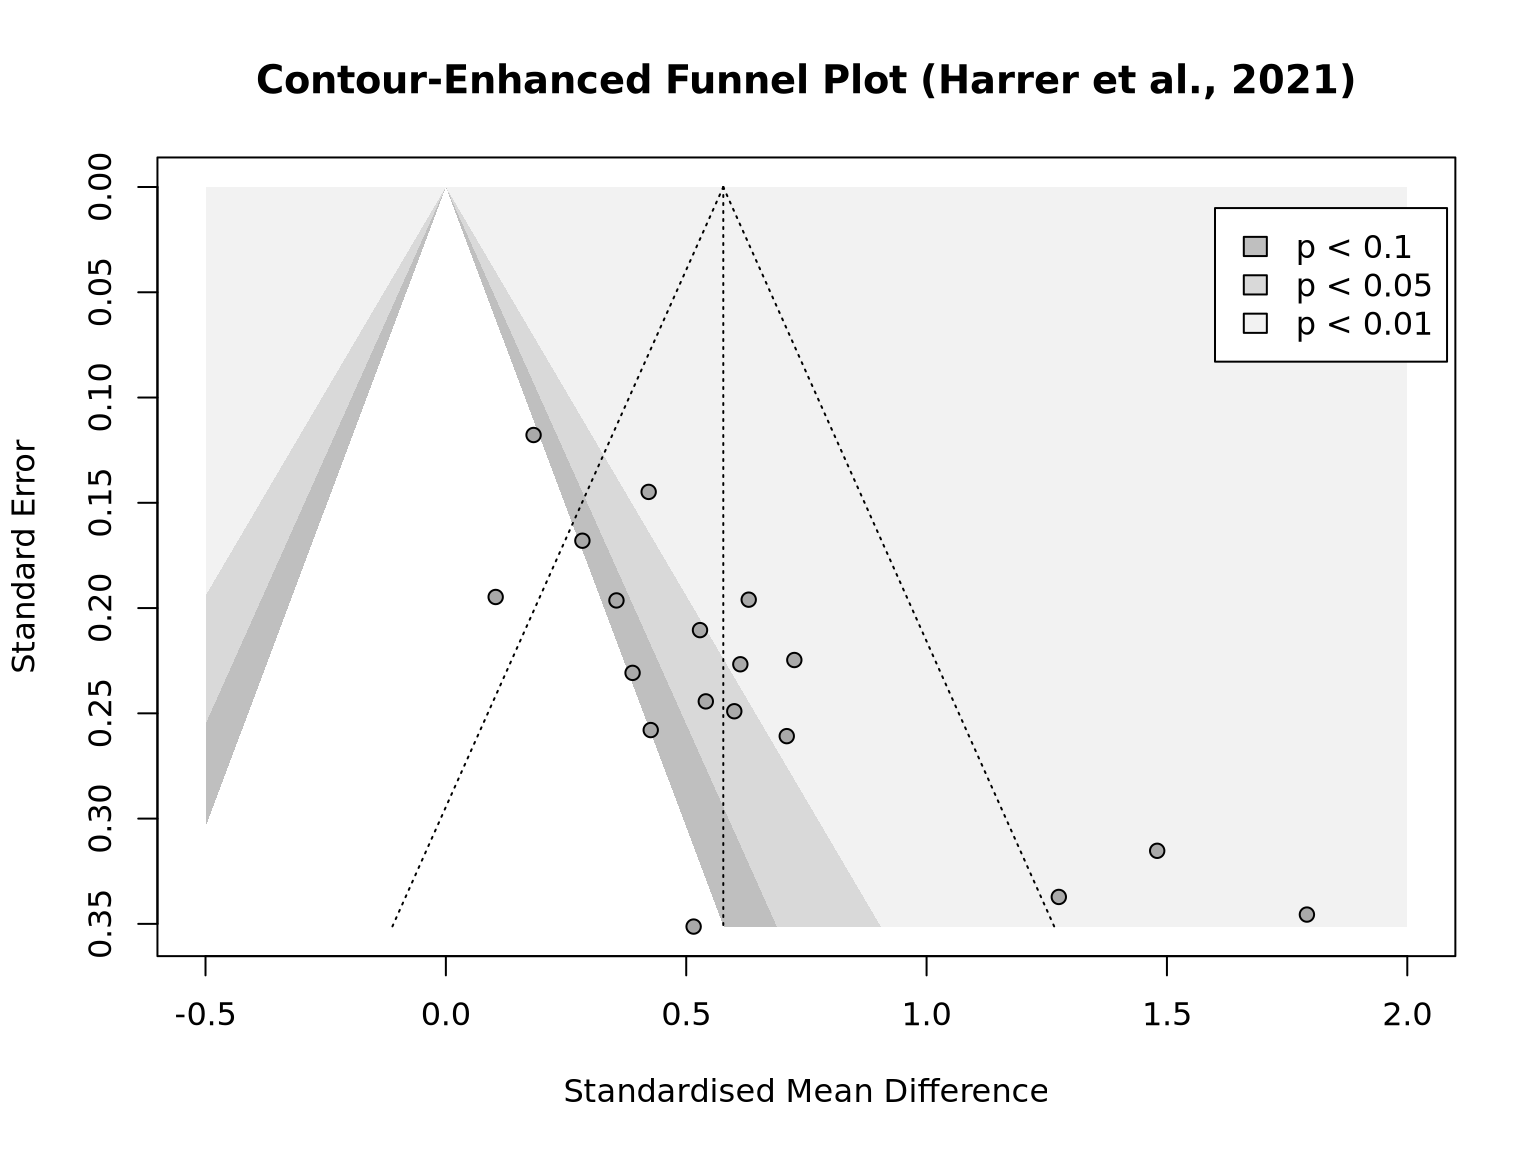
\includegraphics[width=0.75\linewidth]{field_paper_files/figure-latex/unnamed-chunk-13-1} \end{center}

\begin{itemize}
\tightlist
\item
  Egger's regression test
\end{itemize}

Egger's regression test (\protect\hyperlink{ref-eggerBiasMetaanalysisDetected1997}{Egger et al. 1997}) can help to quantify the extent of asymmetry in funnel plot. The simple linear model is

\begin{equation}
\frac{\hat\theta_k}{SE_{\hat\theta_k}} = \beta_0 + \beta_1 \frac{1}{SE_{\hat\theta_k}}
\end{equation}

In Egger's test, the intercept \(\hat\beta_0\) evaluate the funnel asymmetry. If the hypothesis \(\hat\beta_0=0\)
is rejected, then Egger's test shows the plot is asymmetric.

\begin{itemize}
\tightlist
\item
  Peters' Regression Test
\end{itemize}

For binary response, Peters' regression test (\protect\hyperlink{ref-petersComparisonTwoMethods2006}{Peters et al. 2006}) use a weighted simple linear model

\begin{equation}
\log\psi_k =  \beta_0 + \beta_1\frac{1}{n_k}
\end{equation}

where \(\log\psi_k\) represent the log transformation on odds ratios, risk ratios, or proportions.
the predictor is the inverse of the sample size \(n_k\) in \(k\)th study.
When fitting the model, each \(1/n_k\) is assigned a weight \(w_k\), depending on its event counts in treatment group \(a_k\) and control group \(c_k\), non-event counts in treatment group \(c_k\) and control group \(d_k\).

\begin{equation}
w_k = \frac{1}{\left(\dfrac{1}{a_k+c_k}+\dfrac{1}{b_k+d_k}\right)}
\end{equation}

Peters' test uses \(\beta_1\) instead of the intercept to test asymmetry. When the test rejects the hypothesis of \(\beta_1 = 0\), the asymmetry may exist.
For small sample size \(K<10\), Eggers' or Peters' test may fail to identify the asymmetry (\protect\hyperlink{ref-sterneRecommendationsExaminingInterpreting2011}{Sterne et al. 2011}).

\begin{itemize}
\tightlist
\item
  Trim and Fill Method
\end{itemize}

Duval and Tweedie trim and fill method (\protect\hyperlink{ref-duvalTrimFillSimple2000}{Duval and Tweedie 2000}) is a technique of eliminating publication bias.
It is an data imputation method by repeating two steps. The first step of trimming tries to identify the outliers and reevaluate the estimates. In the second step of filling, the trimmed points are adjusted by the expected bias and mirror to the opposite side. Then the mean effect is recalculated based on all points.

This method is based on a strong assumption that the publication bias is the only reason of asymmetry.
It will fail when the cross-study heterogeneity is large (\protect\hyperlink{ref-simonsohnPcurveKeyFiledrawer2014}{Simonsohn, Nelson, and Simmons 2014}).

\begin{itemize}
\tightlist
\item
  PET-PEESE
\end{itemize}

PET-PEESE method (\protect\hyperlink{ref-stanleyMetaregressionApproximationsReduce2014}{Stanley and Doucouliagos 2014}) includes two parts of the precision-effect test (PET) and the precision-effect estimate with standard error (PEESE)
Both of them are simple linear model with response of effect size and predictor of standard error.And the weights are still the inverse of the variance \(w_k= 1/s_k^2\).

\begin{equation}
\begin{split}
\theta_k = \beta_0 + \beta_1\mathrm{SE}_{\theta_k} &\quad \text{PET}\\
\theta_k = \beta_0 + \beta_1\mathrm{SE}_{\theta_k}^2 &\quad \text{PEESE}
\end{split}
\label{eq:pet-peese}
\end{equation}

In the PET part, intercept \(\hat\beta_0\) is used to examine whether the effect size is zero.
If the hypothesis of \(\beta_0=0\) is rejected in PET model, then use the expected \(\hat\beta_0\) in PEESE model as the corrected effect size.
the PET-PEESE method does not perform well for the meta-analysis with small sample size or high cross-study heterogeneity (\protect\hyperlink{ref-carterCorrectingBiasPsychology2019}{Carter et al. 2019}).

\begin{itemize}
\tightlist
\item
  Rücker's Limit Meta-Analysis Method
\end{itemize}

limit meta-analysis by \protect\hyperlink{ref-ruckerTreatmenteffectEstimatesAdjusted2011}{Rücker et al.} (\protect\hyperlink{ref-ruckerTreatmenteffectEstimatesAdjusted2011}{2011}) tries to shrink the publication bias by adding an adjusting term.

\begin{equation}
\hat\theta^*_k =  \hat\mu + \sqrt{\dfrac{\tau^2}{SE^2_k + \tau^2}}(\hat\theta_k - \hat\mu)
\end{equation}

where \(\hat\theta^*_k\) is adjusted expected effect size of study \(k\). \(\hat\theta_k\) is the original expected effect size of study \(k\). \(\hat\mu\) is the expected value of mean effects. \(SE^2_k\) is still the observed variance of \(k\) and \(tau^2\) is the cross-study variance.

\begin{center}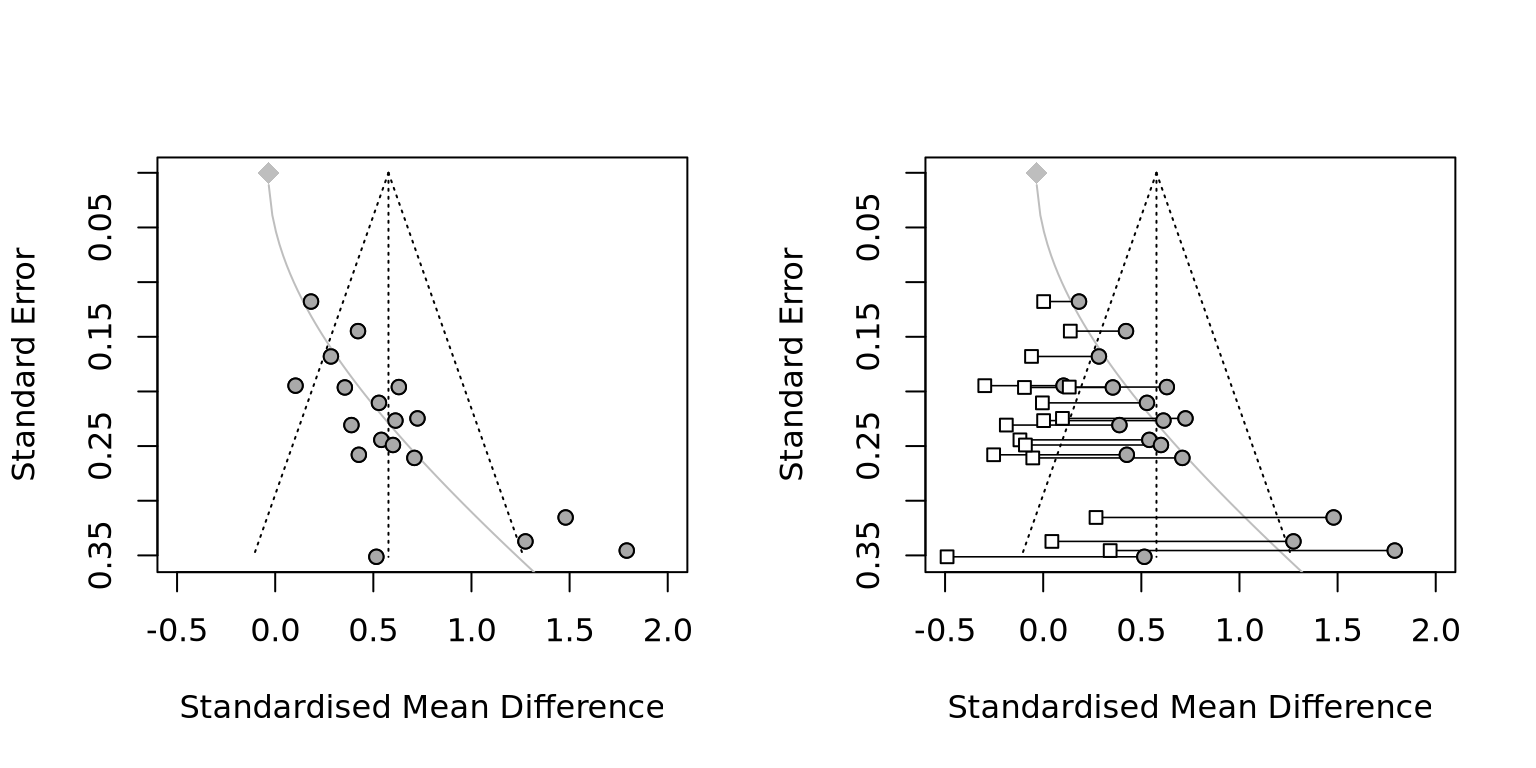
\includegraphics{field_paper_files/figure-latex/unnamed-chunk-14-1} \end{center}

The gray curve shows that the magnitude of expected bias is a monotone increasing function of standard error. Every observations' effects are adjusted by this curve.

\hypertarget{p-value-based-methods}{%
\subsection{P value-based Methods}\label{p-value-based-methods}}

\begin{itemize}
\tightlist
\item
  P-Curve
\end{itemize}

Since the studies with significant results (p-value \textless{} 0.05) tend to be published, either due to the authors or reviewers, the distribution of p-values in the published papers should be exceptional.
P-Curve methods is straightforward by examining whether the p-values in selected studies follows a ``reasonable'' distribution.

In a simulation test, \protect\hyperlink{ref-harrer2021doing}{Harrer et al.} (\protect\hyperlink{ref-harrer2021doing}{2021}) show that the simulated p-values by sampling from a standard normal distribution follows a exponential distribution. When the true effect size is large, the distribution is highly right skewed. Along with the effect size decreasing , the distribution has a longer and longer tail until it becomes an uniform distribution. while another influencing factor is the sample size \(n\). Larger \(n\) will lead to shorter tail.

Based on this assumption, the distribution of p-value in p-hacking studies will be left skewed.
P-curve only shows that the distribution of p-value associates with effect size and sample size.
But the true distribution is still unknown.

\begin{figure}

{\centering 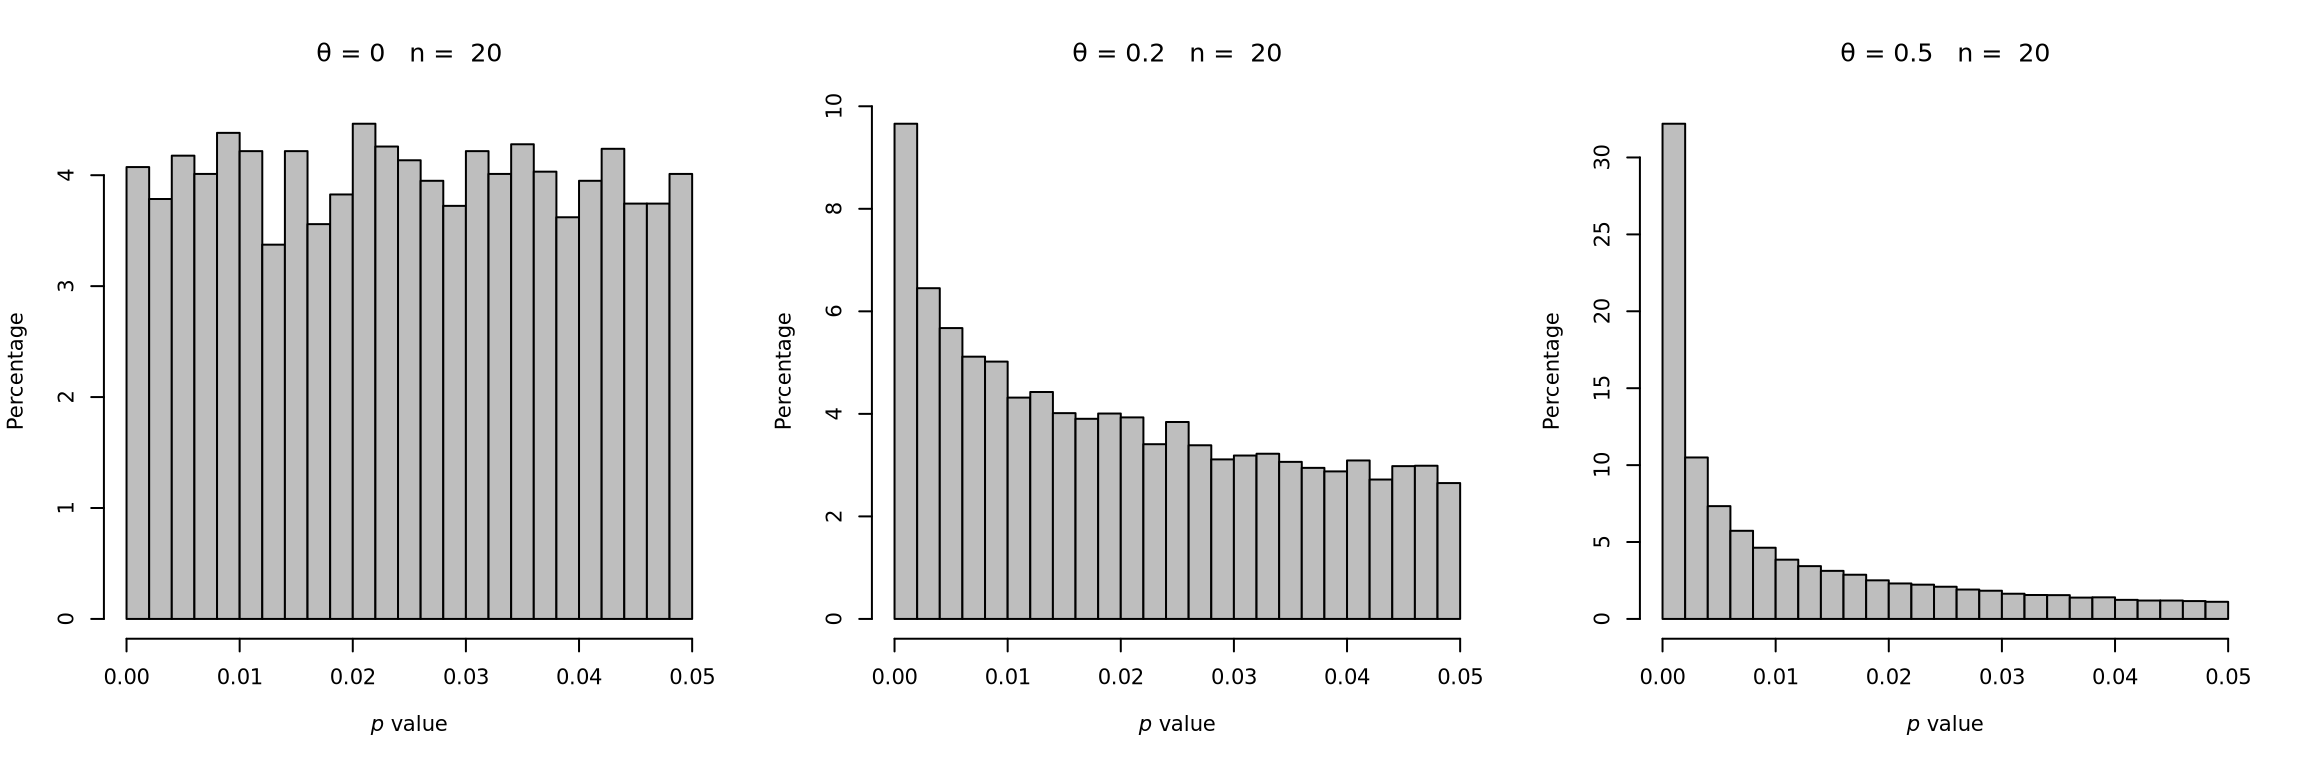
\includegraphics[width=1\linewidth]{field_paper_files/figure-latex/pcurve-1} 

}

\caption{P-curves for varying study sample size and true effect.}\label{fig:pcurve}
\end{figure}

\begin{itemize}
\tightlist
\item
  Test for Right-Skewness
\end{itemize}

It is hard to know the true distribution of p-values but it is easy to test whether the effect size equals zero or not.
Here converts the p-value to a proportion of pp-value as \(pp=p/\alpha\) where \(\alpha\) is the significance level.
Using Fisher's method,the null hypothesis is no right-skewness. If the null hayothesis is rejected, that means the effect exists.

\begin{equation}
\chi^2_{2K} = -2 \sum^K_{k=1} \log(pp_k)
\end{equation}

\begin{itemize}
\tightlist
\item
  Test for 33\% Power (flatness of the p-curve)
\end{itemize}

Test for 33\% power starts from another direction. Based on the properties of the non-central distribution of \(F\), \(t\), or \(\chi^2\), the null hypothesis is that a small effect exists, or the p-curve is slightly right skewed.

The 33\% power is a rough threshold. Statistical power \(1-\beta\) means a probability of correctly rejecting the null hypothesis. It is equivalent with a 66\% probability of Type II error, also called ``false negative.''
For example, in a paired t-test for normal distributed data, if the alternative hypothesis is true and the true difference \(\theta=\theta_0\). Then the power is

\begin{equation}
\begin{split}
&Pr(\frac{\hat\theta-0}{SE}>\Phi^{-1}(0.95)|\theta=\theta_0)\\
=&Pr(\frac{\hat\theta-\theta}{SE}>1.64-\frac{\theta}{SE}|\theta=\theta_0)\\
=&1-Pr(\frac{\hat\theta-\theta}{SE}<1.64-\frac{\theta}{SE}|\theta=\theta_0)>0.33
\end{split}
\label{eq:33power}
\end{equation}

When the sample size is large, \(\frac{\hat\theta-\theta}{SE}\) asymptotically follow a standard normal distribution. Then

\begin{equation}
\frac{\theta}{SE}>1.64-\Phi^{-1}(0.66)\approx 1.2324
\end{equation}

When the right-skewness test cannot reject \(\theta=0\), then the flatness test may reject that the effect size is large. If both of the two tests are not significant, then the evidence is insufficient for any conclusion.
Note that the flatness test depends on how to define a small value of \(\theta\).
Another alternative method is the Kolmogorov-Smirnov (KS) test by comparing a sample with a reference probability distribution.

\begin{itemize}
\tightlist
\item
  Selection Models
\end{itemize}

Selection Model supposes a probability density function \(f(\theta)\) can reflect the true distribution of effect sizes without publication bias.
The background assumption still is the observed effect sizes \(\theta_k \sim N(\mu,\sigma^2+\tau^2)\), sampling error \(\sigma^2\), and cross-study heterogeneity variance \(\tau^2\).
By assuming a weight function \(w(p_k)\) of p-value \(p_k\) can represent the mechanism of publication bias, then the adjusted function \(f^*(\theta)\) should be consistent with the observed data.

\begin{equation}
f^*(\theta_k) = \frac{w(p_k)f(\theta_k)}{\int w(p_k) f(\theta_k) d\theta_k}
\end{equation}

A straightforward choice of \(w(p_k)\) is a \textbf{step function} (\protect\hyperlink{ref-hedgesEstimatingEffectSize1996}{Hedges and Vevea 1996}).
Since \(\alpha_{1,2,3}=0.05, 0.1, 0.5\) is the common critical values, the step function uses them as cut points and divide the range of p-value \(p\in(0,1)\) into four segments.
Using maximum likelihood, the probability for each segment can be estimated such as \(w_{1,2,3,4}=1,0.8,0.6,0.35\), and the best fitted \(f^*(\theta)\) can recover the true function \(f(\theta)\) and unbiased estimates of \(\hat\mu\) and \(\hat\tau^2\)

\begin{figure}

{\centering 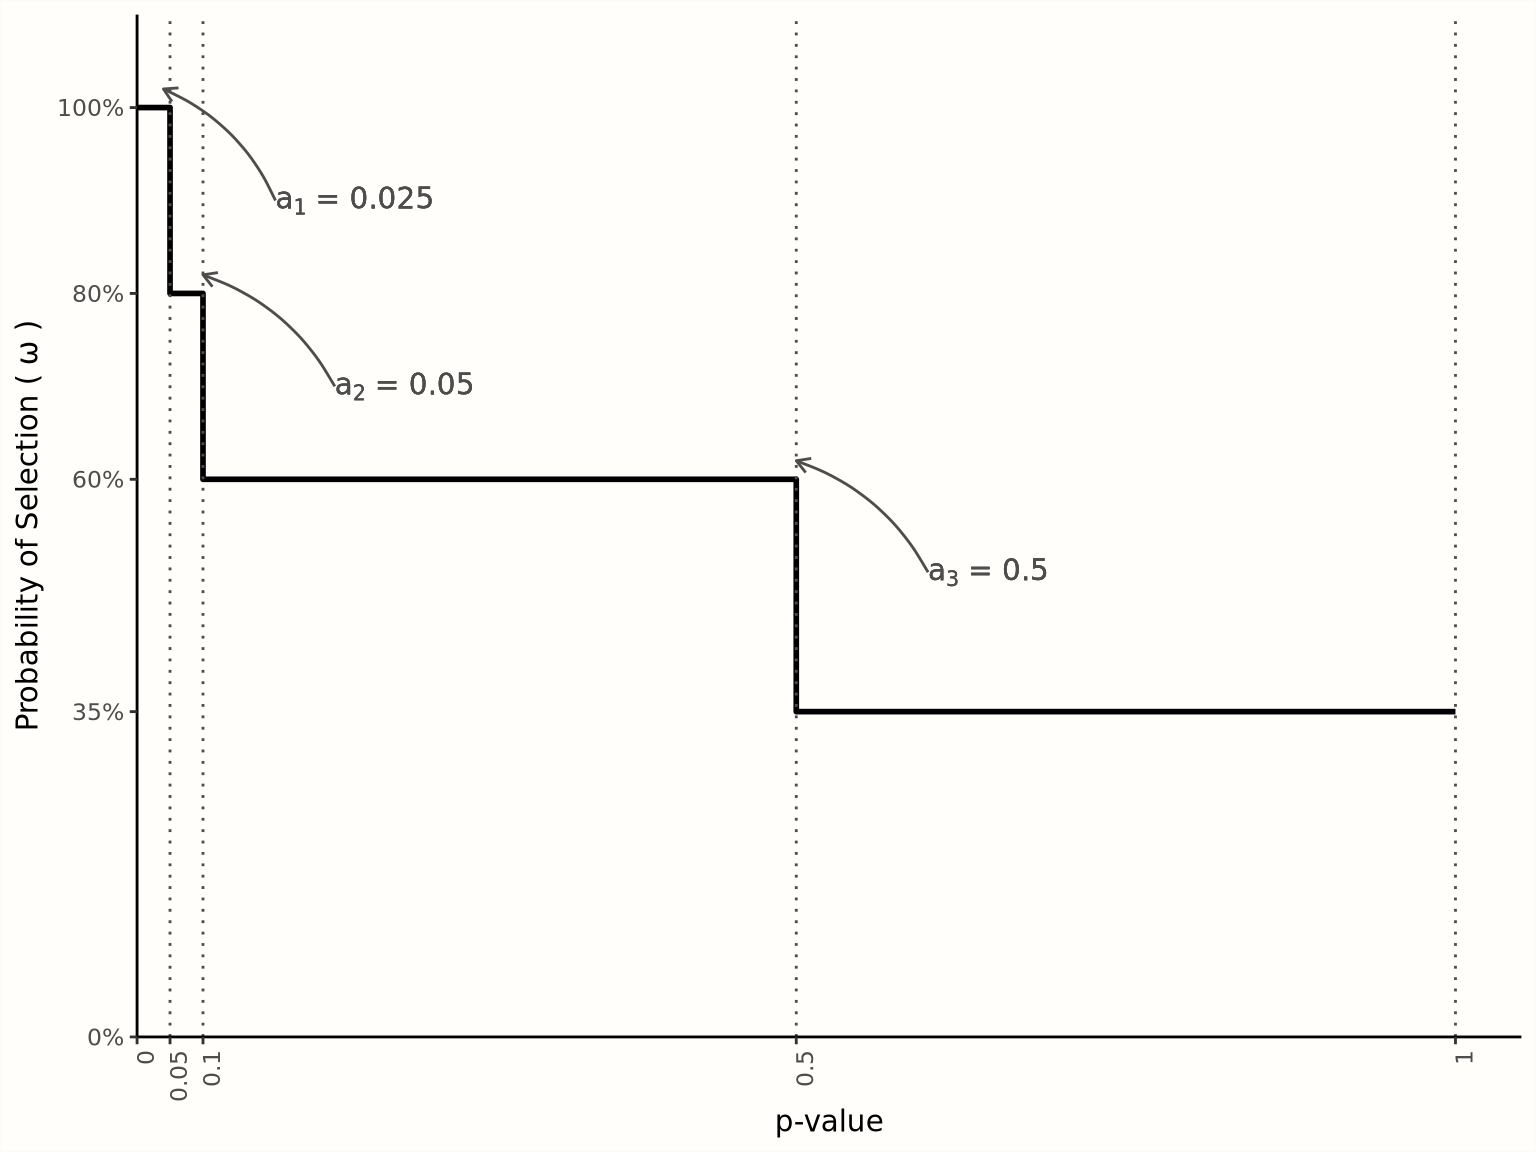
\includegraphics[width=0.6\linewidth]{field_paper_files/figure-latex/stepcurve-1} 

}

\caption{Selection model based on a step function.}\label{fig:stepcurve}
\end{figure}

\textbf{Three-parameter model} assumes only one cut-point (\protect\hyperlink{ref-mcshaneAdjustingPublicationBias2016}{McShane, Böckenholt, and Hansen 2016}).
That is \(\alpha=0.025\), which means p-value \(=0.05\) in a two-sides test. Then the weight function only has two segments. The three parameters inlude the true effect \(\mu\), the cross-study heterogeneity variance \(\tau^2\), and the probability of the second segment \(w_2\).

\textbf{Fixed weights selection model} completely assigns all the cut points and their weight (\protect\hyperlink{ref-veveaPublicationBiasResearch2005}{Vevea and Woods 2005}).
This method allows to fit a very flexible selection model.
On the contrary, one can also assume a global monotonic decreasing distribution such as half-normal, logistic, negative-exponential, etc.

All of these methods are based on the assumed distribution under publication bias being correct.
Without sufficient cases and test, identifying the true distribution in one specific field is difficult.
Especially, when cross-study heterogeneity is high, such as \(I^2\approx\) 75\%, these approaches are not reliable (\protect\hyperlink{ref-vanaertConductingMetaAnalysesBased2016}{van Aert, Wicherts, and van Assen 2016}).
Therefore, when the meta-analyses of travel-urban form studies show the high heterogeneity, it is hard to verify and eliminate the possible publication bias.

\hypertarget{refs}{}
\begin{CSLReferences}{1}{0}
\leavevmode\vadjust pre{\hypertarget{ref-vanaertConductingMetaAnalysesBased2016}{}}%
Aert, Robbie C. M. van, Jelte M. Wicherts, and Marcel A. L. M. van Assen. 2016. {``Conducting {Meta}-{Analyses Based} on p {Values}: Reservations and {Recommendations} for {Applying} p-{Uniform} and p-{Curve}.''} \emph{Perspectives on Psychological Science} 11 (5): 713--29. \url{https://doi.org/10.1177/1745691616650874}.

\leavevmode\vadjust pre{\hypertarget{ref-ajzenTheoryPlannedBehavior1991}{}}%
Ajzen, Icek. 1991. {``The Theory of Planned Behavior.''} \emph{Organizational Behavior and Human Decision Processes}, Theories of {Cognitive Self}-{Regulation}, 50 (2): 179--211. \url{https://doi.org/10.1016/0749-5978(91)90020-T}.

\leavevmode\vadjust pre{\hypertarget{ref-ajzenAttitudebehaviorRelationsTheoretical1977}{}}%
Ajzen, Icek, and Martin Fishbein. 1977. {``Attitude-Behavior Relations: A Theoretical Analysis and Review of Empirical Research.''} \emph{Psychological Bulletin} 84 (5): 888--918. \url{https://doi.org/10.1037/0033-2909.84.5.888}.

\leavevmode\vadjust pre{\hypertarget{ref-amrheinSearchingElusiveAggregation1995}{}}%
Amrhein, C G. 1995. {``Searching for the {Elusive Aggregation Effect}: Evidence from {Statistical Simulations}.''} \emph{Environment and Planning A: Economy and Space} 27 (1): 105--19. \url{https://doi.org/10.1068/a270105}.

\leavevmode\vadjust pre{\hypertarget{ref-kittelson2013evaluating}{}}%
Associates, Kittelson \&, and Second Strategic Highway Research Program (US). 2013. \emph{Evaluating Alternative Operations Strategies to Improve Travel Time Reliability}. Transportation Research Board.

\leavevmode\vadjust pre{\hypertarget{ref-astonExploringBuiltEnvironment2021}{}}%
Aston, Laura, Graham Currie, Alexa Delbosc, Md Kamruzzaman, and David Teller. 2021. {``Exploring Built Environment Impacts on Transit Use -- an Updated Meta-Analysis.''} \emph{Transport Reviews} 41 (1): 73--96. \url{https://doi.org/10.1080/01441647.2020.1806941}.

\leavevmode\vadjust pre{\hypertarget{ref-astonStudyDesignImpacts2020}{}}%
Aston, Laura, Graham Currie, Md. Kamruzzaman, Alexa Delbosc, and David Teller. 2020. {``Study Design Impacts on Built Environment and Transit Use Research.''} \emph{Journal of Transport Geography} 82 (January): 102625. \url{https://doi.org/10.1016/j.jtrangeo.2019.102625}.

\leavevmode\vadjust pre{\hypertarget{ref-barbosaHumanMobilityModels2018}{}}%
Barbosa, Hugo, Marc Barthelemy, Gourab Ghoshal, Charlotte R. James, Maxime Lenormand, Thomas Louail, Ronaldo Menezes, José J. Ramasco, Filippo Simini, and Marcello Tomasini. 2018. {``Human Mobility: Models and Applications.''} \emph{Physics Reports}, Human mobility: Models and applications, 734 (March): 1--74. \url{https://doi.org/10.1016/j.physrep.2018.01.001}.

\leavevmode\vadjust pre{\hypertarget{ref-ben-akivaDiscreteChoiceAnalysis1985}{}}%
Ben-Akiva, Moshe, and Steven R. Lerman. 1985. \emph{Discrete {Choice Analysis}: Theory and {Application} to {Travel Demand}}. {MIT Press}. \url{https://books.google.com?id=7L34DwAAQBAJ}.

\leavevmode\vadjust pre{\hypertarget{ref-ben-akivaHybridChoiceModels2002}{}}%
Ben-Akiva, Moshe, Daniel Mcfadden, Kenneth Train, Joan Walker, Chandra Bhat, Michel Bierlaire, Denis Bolduc, et al. 2002. {``Hybrid {Choice Models}: Progress and {Challenges}.''} \emph{Marketing Letters} 13 (3): 163--75. \url{https://doi.org/10.1023/A:1020254301302}.

\leavevmode\vadjust pre{\hypertarget{ref-ben-arivaMETHODOLOGYSHORTRANGETRAVEL1977}{}}%
Ben-Ariva, M., and T. J. Atherton. 1977. {``{METHODOLOGY FOR SHORT}-{RANGE TRAVEL DEMAND PREDICTIONS}. {ANALYSIS OF CARPOOLING INCENTIVES}.''} \emph{Journal of Transport Economics and Policy} 11 (Analytic, 3). \url{http://trid.trb.org/view/61044}.

\leavevmode\vadjust pre{\hypertarget{ref-bentoEffectsUrbanSpatial2005}{}}%
Bento, Antonio M., Maureen L. Cropper, Ahmed Mushfiq Mobarak, and Katja Vinha. 2005. {``The {Effects} of {Urban Spatial Structure} on {Travel Demand} in the {United States}.''} \emph{The Review of Economics and Statistics} 87 (3): 466--78. \url{https://doi.org/10.1162/0034653054638292}.

\leavevmode\vadjust pre{\hypertarget{ref-bienInflatedMultivariateInteger2011}{}}%
Bien, Katarzyna, Ingmar Nolte, and Winfried Pohlmeier. 2011. {``An Inflated Multivariate Integer Count Hurdle Model: An Application to Bid and Ask Quote Dynamics.''} \emph{Journal of Applied Econometrics} 26 (4): 669--707. \url{https://doi.org/10.1002/jae.1122}.

\leavevmode\vadjust pre{\hypertarget{ref-boarnetInfluenceLandUse2001}{}}%
Boarnet, Marlon, and Randall Crane. 2001. {``The Influence of Land Use on Travel Behavior: Specification and Estimation Strategies.''} \emph{Transportation Research Part A: Policy and Practice} 35 (9): 823--45. \url{https://doi.org/10.1016/S0965-8564(00)00019-7}.

\leavevmode\vadjust pre{\hypertarget{ref-bonettPointbiserialCorrelationInterval2020}{}}%
Bonett, Douglas G. 2020. {``Point-Biserial Correlation: Interval Estimation, Hypothesis Testing, Meta-Analysis, and Sample Size Determination.''} \emph{British Journal of Mathematical and Statistical Psychology} 73 (S1): 113--44. \url{https://doi.org/10.1111/bmsp.12189}.

\leavevmode\vadjust pre{\hypertarget{ref-borensteinIntroductionMetaAnalysis2021}{}}%
Borenstein, Michael, Larry V. Hedges, Julian P. T. Higgins, and Hannah R. Rothstein. 2021. \emph{Introduction to {Meta}-{Analysis}}. {John Wiley \& Sons}. \url{https://books.google.com?id=pdQnEAAAQBAJ}.

\leavevmode\vadjust pre{\hypertarget{ref-brockmannScalingLawsHuman2006}{}}%
Brockmann, D., L. Hufnagel, and T. Geisel. 2006. {``The Scaling Laws of Human Travel.''} \emph{Nature} 439 (7075, 7075): 462--65. \url{https://doi.org/10.1038/nature04292}.

\leavevmode\vadjust pre{\hypertarget{ref-buchananEffectUrbanGrowth2006}{}}%
Buchanan, Nick, Ross Barnett, Simon Kingham, and Doug Johnston. 2006. {``The Effect of Urban Growth on Commuting Patterns in {Christchurch}, {New Zealand}.''} \emph{Journal of Transport Geography} 14 (5): 342--54. \url{https://doi.org/10.1016/j.jtrangeo.2005.10.008}.

\leavevmode\vadjust pre{\hypertarget{ref-cambridge2003providing}{}}%
Cambridge Systematics, Texas Transportation Institute, Univ. of Washington, and Dowling Associates. 2003. {``Providing a Highway System with Reliable Travel Times.''} Transportation Research Board of the National Academies Washington, DC.

\leavevmode\vadjust pre{\hypertarget{ref-camererAdvancesBehavioralEconomics2004}{}}%
Camerer, Colin F., George Loewenstein, and Matthew Rabin. 2004. \emph{Advances in {Behavioral Economics}}. {Princeton University Press}. \url{https://books.google.com?id=xWKYDwAAQBAJ}.

\leavevmode\vadjust pre{\hypertarget{ref-carterCorrectingBiasPsychology2019}{}}%
Carter, Evan C., Felix D. Schönbrodt, Will M. Gervais, and Joseph Hilgard. 2019. {``Correcting for {Bias} in {Psychology}: A {Comparison} of {Meta}-{Analytic Methods}.''} \emph{Advances in Methods and Practices in Psychological Science} 2 (2): 115--44. \url{https://doi.org/10.1177/2515245919847196}.

\leavevmode\vadjust pre{\hypertarget{ref-casellaStatisticalInference2002}{}}%
Casella, George, and Roger L. Berger. 2002. \emph{Statistical Inference}. 2nd ed. {Australia ; Pacific Grove, CA}: {Thomson Learning}.

\leavevmode\vadjust pre{\hypertarget{ref-cerveroTravelDemand3Ds1997}{}}%
Cervero, Robert, and Kara Kockelman. 1997. {``Travel Demand and the {3Ds}: Density, Diversity, and Design.''} \emph{Transportation Research Part D: Transport and Environment} 2 (3): 199--219. \url{https://doi.org/10.1016/S1361-9209(97)00009-6}.

\leavevmode\vadjust pre{\hypertarget{ref-chatmanHowDensityMixed2003}{}}%
Chatman, Daniel G. 2003. {``How {Density} and {Mixed Uses} at the {Workplace Affect Personal Commercial Travel} and {Commute Mode Choice}.''} \emph{Transportation Research Record} 1831 (1): 193--201. \url{https://doi.org/10.3141/1831-22}.

\leavevmode\vadjust pre{\hypertarget{ref-chenHierarchicalScalingSystems2018}{}}%
Chen, Yanguang, and Bin Jiang. 2018. {``Hierarchical {Scaling} in {Systems} of {Natural Cities}.''} \emph{Entropy} 20 (6, 6): 432. \url{https://doi.org/10.3390/e20060432}.

\leavevmode\vadjust pre{\hypertarget{ref-cliftonGettingHereThere2017}{}}%
Clifton, Kelly J. 2017. {``Getting {From Here} to {There}: Comment on {`{Does Compact Development Make People Drive Less}?'}.''} \emph{Journal of the American Planning Association} 83 (2): 148--51. \url{https://doi.org/10.1080/01944363.2017.1290494}.

\leavevmode\vadjust pre{\hypertarget{ref-cochranMethodsStrengtheningCommon1954}{}}%
Cochran, William G. 1954. {``Some {Methods} for {Strengthening} the {Common} Chi-Squared {Tests}.''} \emph{Biometrics} 10 (4): 417--51. \url{https://doi.org/10.2307/3001616}.

\leavevmode\vadjust pre{\hypertarget{ref-vandecoeveringReevaluatingImpactUrban2006}{}}%
Coevering, Paul van de, and Tim Schwanen. 2006. {``Re-Evaluating the Impact of Urban Form on Travel Patternsin {Europe} and {North}-{America}.''} \emph{Transport Policy} 13 (3): 229--39. \url{https://doi.org/10.1016/j.tranpol.2005.10.001}.

\leavevmode\vadjust pre{\hypertarget{ref-cohenStatisticalPowerAnalysis1988}{}}%
Cohen, Jacob. 1988. \emph{Statistical {Power Analysis} for the {Behavioral Sciences}}. 2nd ed. {New York}: {Routledge}. \url{https://doi.org/10.4324/9780203771587}.

\leavevmode\vadjust pre{\hypertarget{ref-cuijpersMetaanalysesMentalHealth2016}{}}%
Cuijpers, Pim. 2016. \emph{Meta-Analyses in Mental Health Research: A Practical Guide}.

\leavevmode\vadjust pre{\hypertarget{ref-devosIndirectEffectBuilt2021}{}}%
De Vos, Jonas, Long Cheng, Md. Kamruzzaman, and Frank Witlox. 2021. {``The Indirect Effect of the Built Environment on Travel Mode Choice: A Focus on Recent Movers.''} \emph{Journal of Transport Geography} 91 (February): 102983. \url{https://doi.org/10.1016/j.jtrangeo.2021.102983}.

\leavevmode\vadjust pre{\hypertarget{ref-dingNonlinearAssociationsZonal2021}{}}%
Ding, Chuan, Xinyu Cao, Bin Yu, and Yang Ju. 2021. {``Non-Linear Associations Between Zonal Built Environment Attributes and Transit Commuting Mode Choice Accounting for Spatial Heterogeneity.''} \emph{Transportation Research Part A: Policy and Practice} 148 (June): 22--35. \url{https://doi.org/10.1016/j.tra.2021.03.021}.

\leavevmode\vadjust pre{\hypertarget{ref-dingInfluencesBuiltEnvironment2017}{}}%
Ding, Chuan, Sabyasachee Mishra, Guangquan Lu, Jiawen Yang, and Chao Liu. 2017. {``Influences of Built Environment Characteristics and Individual Factors on Commuting Distance: A Multilevel Mixture Hazard Modeling Approach.''} \emph{Transportation Research Part D: Transport and Environment} 51 (March): 314--25. \url{https://doi.org/10.1016/j.trd.2017.02.002}.

\leavevmode\vadjust pre{\hypertarget{ref-dingExploringInfluenceBuilt2017}{}}%
Ding, Chuan, Donggen Wang, Chao Liu, Yi Zhang, and Jiawen Yang. 2017. {``Exploring the Influence of Built Environment on Travel Mode Choice Considering the Mediating Effects of Car Ownership and Travel Distance.''} \emph{Transportation Research Part A: Policy and Practice} 100 (June): 65--80. \url{https://doi.org/10.1016/j.tra.2017.04.008}.

\leavevmode\vadjust pre{\hypertarget{ref-domencichURBANTRAVELDEMAND1975}{}}%
Domencich, T. A., and D. McFadden. 1975. {``{URBAN TRAVEL DEMAND} - {A BEHAVIORAL ANALYSIS},''} no. Monograph. \url{http://trid.trb.org/view/48594}.

\leavevmode\vadjust pre{\hypertarget{ref-dujardinHometoworkCommutingUrban2012}{}}%
Dujardin, S., F. Pirart, F. Brévers, A. -F. Marique, and J. Teller. 2012. {``Home-to-Work Commuting, Urban Form and Potential Energy Savings: A Local Scale Approach to Regional Statistics.''} \emph{Transportation Research Part A: Policy and Practice} 46 (7): 1054--65. \url{https://doi.org/10.1016/j.tra.2012.04.010}.

\leavevmode\vadjust pre{\hypertarget{ref-duvalTrimFillSimple2000}{}}%
Duval, Sue, and Richard Tweedie. 2000. {``Trim and {Fill}: A {Simple Funnel}-{Plot}--{Based Method} of {Testing} and {Adjusting} for {Publication Bias} in {Meta}-{Analysis}.''} \emph{Biometrics} 56 (2): 455--63. \url{https://doi.org/10.1111/j.0006-341X.2000.00455.x}.

\leavevmode\vadjust pre{\hypertarget{ref-edwardsTheoryDecisionMaking1954}{}}%
Edwards, Ward. 1954. {``The Theory of Decision Making.''} \emph{Psychological Bulletin} 51 (4): 380--417. \url{https://doi.org/10.1037/h0053870}.

\leavevmode\vadjust pre{\hypertarget{ref-eggerBiasMetaanalysisDetected1997}{}}%
Egger, Matthias, George Davey Smith, Martin Schneider, and Christoph Minder. 1997. {``Bias in Meta-Analysis Detected by a Simple, Graphical Test.''} \emph{BMJ} 315 (7109): 629--34. \url{https://doi.org/10.1136/bmj.315.7109.629}.

\leavevmode\vadjust pre{\hypertarget{ref-ewingTravelBuiltEnvironment2001}{}}%
Ewing, Reid, and Robert Cervero. 2001. {``Travel and the {Built Environment}: A {Synthesis}.''} \emph{Transportation Research Record: Journal of the Transportation Research Board} 1780 (January): 87--114. \url{https://doi.org/10.3141/1780-10}.

\leavevmode\vadjust pre{\hypertarget{ref-ewingTravelBuiltEnvironment2010}{}}%
---------. 2010. {``Travel and the {Built Environment}.''} \emph{Journal of the American Planning Association} 76 (3): 265--94. \url{https://doi.org/10.1080/01944361003766766}.

\leavevmode\vadjust pre{\hypertarget{ref-ewingDoesCompactDevelopment2017}{}}%
---------. 2017. {``{`{Does Compact Development Make People Drive Less}?'} {The Answer Is Yes}.''} \emph{Journal of the American Planning Association} 83 (1): 19--25. \url{https://doi.org/10.1080/01944363.2016.1245112}.

\leavevmode\vadjust pre{\hypertarget{ref-ewingUrbanSprawlRisk2016}{}}%
Ewing, Reid, Shima Hamidi, and James B Grace. 2016. {``Urban Sprawl as a Risk Factor in Motor Vehicle Crashes.''} \emph{Urban Studies} 53 (2): 247--66. \url{https://doi.org/10.1177/0042098014562331}.

\leavevmode\vadjust pre{\hypertarget{ref-ewingTestingNewmanKenworthy2018}{}}%
Ewing, Reid, Shima Hamidi, Guang Tian, David Proffitt, Stefania Tonin, and Laura Fregolent. 2018. {``Testing {Newman} and {Kenworthy}'s {Theory} of {Density} and {Automobile Dependence}.''} \emph{Journal of Planning Education and Research} 38 (2): 167--82. \url{https://doi.org/10.1177/0739456X16688767}.

\leavevmode\vadjust pre{\hypertarget{ref-ewingRelationshipUrbanSprawl2014}{}}%
Ewing, Reid, Gail Meakins, Shima Hamidi, and Arthur C. Nelson. 2014. {``Relationship Between Urban Sprawl and Physical Activity, Obesity, and Morbidity -- {Update} and Refinement.''} \emph{Health \& Place} 26 (March): 118--26. \url{https://doi.org/10.1016/j.healthplace.2013.12.008}.

\leavevmode\vadjust pre{\hypertarget{ref-ewingReducingVehicleMiles2020}{}}%
Ewing, Reid, Keunhyun Park, Sadegh Sabouri, Torrey Lyons, Keuntae Kim, Dong-ah Choi, Katherine Daly, and Roya Ghasrodashti. 2020. {``Reducing {Vehicle Miles Traveled}, {Encouraging Walk Trips}, and {Facilitating Efficient Trip Chains Through Polycentric Development}.''} \emph{TREC Final Reports}, October. \url{https://doi.org/10.15760/trec.255}.

\leavevmode\vadjust pre{\hypertarget{ref-ewingVaryingInfluencesBuilt2015}{}}%
Ewing, Reid, Guang Tian, JP Goates, Ming Zhang, Michael J Greenwald, Alex Joyce, John Kircher, and William Greene. 2015. {``Varying Influences of the Built Environment on Household Travel in 15 Diverse Regions of the {United States}.''} \emph{Urban Studies} 52 (13): 2330--48. \url{https://doi.org/10.1177/0042098014560991}.

\leavevmode\vadjust pre{\hypertarget{ref-fanisThreeStudiesThat2019}{}}%
Fanis, Grammenos. 2019. {``Three {Studies That Show Density Doesn}'t {Determine Car Travel}.''} {Planetizen - Urban Planning News, Jobs, and Education}. September 30, 2019. \url{https://www.planetizen.com/features/106433-three-studies-show-density-doesnt-determine-car-travel}.

\leavevmode\vadjust pre{\hypertarget{ref-fotheringhamModifiableArealUnit1991}{}}%
Fotheringham, A S, and D W S Wong. 1991. {``The {Modifiable Areal Unit Problem} in {Multivariate Statistical Analysis}.''} \emph{Environment and Planning A: Economy and Space} 23 (7): 1025--44. \url{https://doi.org/10.1068/a231025}.

\leavevmode\vadjust pre{\hypertarget{ref-gardnerPsychologicalCorrelatesCar2008}{}}%
Gardner, Benjamin, and Charles Abraham. 2008. {``Psychological Correlates of Car Use: A Meta-Analysis.''} \emph{Transportation Research Part F: Traffic Psychology and Behaviour} 11 (4): 300--311. \url{https://doi.org/10.1016/j.trf.2008.01.004}.

\leavevmode\vadjust pre{\hypertarget{ref-gehlkeCertainEffectsGrouping1934}{}}%
Gehlke, C. E., and Katherine Biehl. 1934. {``Certain {Effects} of {Grouping} Upon the {Size} of the {Correlation Coefficient} in {Census Tract Material}.''} \emph{Journal of the American Statistical Association} 29 (March): 169--70. \url{https://doi.org/10.1080/01621459.1934.10506247}.

\leavevmode\vadjust pre{\hypertarget{ref-GeographicallyWeightedRegression}{}}%
{``Geographically {Weighted Regression} - an Overview \textbar{} {ScienceDirect Topics}.''} n.d. Accessed August 22, 2021. \url{https://www-sciencedirect-com.proxy.lib.pdx.edu/topics/earth-and-planetary-sciences/geographically-weighted-regression}.

\leavevmode\vadjust pre{\hypertarget{ref-gimRelationshipsLandUse2013}{}}%
Gim, Tae-Hyoung Tommy. 2013. {``The Relationships Between Land Use Measures and Travel Behavior: A Meta-Analytic Approach.''} \emph{Transportation Planning and Technology} 36 (5): 413--34. \url{https://doi.org/10.1080/03081060.2013.818272}.

\leavevmode\vadjust pre{\hypertarget{ref-gimAnalyzingCitylevelEffects2021}{}}%
---------. 2021. {``Analyzing the City-Level Effects of Land Use on Travel Time and {Co2} Emissions: A Global Mediation Study of Travel Time.''} \emph{International Journal of Sustainable Transportation} 0 (0): 1--18. \url{https://doi.org/10.1080/15568318.2021.1901163}.

\leavevmode\vadjust pre{\hypertarget{ref-gomez-lievanoStatisticsUrbanScaling2012}{}}%
Gomez-Lievano, Andres, HyeJin Youn, and Luís M. A. Bettencourt. 2012. {``The {Statistics} of {Urban Scaling} and {Their Connection} to {Zipf}'s {Law}.''} \emph{PLoS One} 7 (7): e40393. https://doi.org/\url{http://dx.doi.org.proxy.lib.pdx.edu/10.1371/journal.pone.0040393}.

\leavevmode\vadjust pre{\hypertarget{ref-gordonGasolineConsumptionCities1989}{}}%
Gordon, Peter, and Harry W. Richardson. 1989. {``Gasoline {Consumption And Cities}: A {Reply}.''} \emph{American Planning Association. Journal of the American Planning Association} 55 (3): 342. \url{http://search.proquest.com/docview/229599978/abstract/FBB96AB65F044006PQ/1}.

\leavevmode\vadjust pre{\hypertarget{ref-gotschiComprehensiveConceptualFramework2017}{}}%
Götschi, Thomas, Audrey de Nazelle, Christian Brand, Regine Gerike, B. Alasya, E. Anaya, I. Avila-Palencia, et al. 2017. {``Towards a {Comprehensive Conceptual Framework} of {Active Travel Behavior}: A {Review} and {Synthesis} of {Published Frameworks}.''} \emph{Current Environmental Health Reports} 4 (3): 286--95. \url{https://doi.org/10.1007/s40572-017-0149-9}.

\leavevmode\vadjust pre{\hypertarget{ref-hackmannEvolutionZipfLaw2020}{}}%
Hackmann, Angelina, and Torben Klarl. 2020. {``The Evolution of {Zipf}'s {Law} for {U}.{S}. Cities.''} \emph{Papers in Regional Science} 99 (3): 841--52. \url{https://doi.org/10.1111/pirs.12498}.

\leavevmode\vadjust pre{\hypertarget{ref-hagerstraandWhatPeopleRegional1970}{}}%
Hägerstraand, Torsten. 1970. {``What {About People} in {Regional Science}?''} \emph{Papers in Regional Science} 24 (1): 7--24. \url{https://doi.org/10.1111/j.1435-5597.1970.tb01464.x}.

\leavevmode\vadjust pre{\hypertarget{ref-hamidiLongitudinalStudyChanges2014}{}}%
Hamidi, Shima, and Reid Ewing. 2014. {``A Longitudinal Study of Changes in Urban Sprawl Between 2000 and 2010 in the {United States}.''} \emph{Landscape and Urban Planning} 128 (August): 72--82. \url{https://doi.org/10.1016/j.landurbplan.2014.04.021}.

\leavevmode\vadjust pre{\hypertarget{ref-hamidiMeasuringSprawlIts2015}{}}%
Hamidi, Shima, Reid Ewing, Ilana Preuss, and Alex Dodds. 2015. {``Measuring {Sprawl} and {Its Impacts}: An {Update}.''} \emph{Journal of Planning Education and Research} 35 (1): 35--50. \url{https://doi.org/10.1177/0739456X14565247}.

\leavevmode\vadjust pre{\hypertarget{ref-handyCriticalAssessmentLiterature2005}{}}%
Handy, Susan. 2005. {``Critical {Assessment} of the {Literature} on the {Relationships Among Transportation}, {Land Use}, and {Physical Activity},''} 102.

\leavevmode\vadjust pre{\hypertarget{ref-handyThoughtsMeaningMark2017}{}}%
---------. 2017. {``Thoughts on the {Meaning} of {Mark Stevens}'s {Meta}-{Analysis}.''} \emph{Journal of the American Planning Association} 83 (1): 26--28. \url{https://doi.org/10.1080/01944363.2016.1246379}.

\leavevmode\vadjust pre{\hypertarget{ref-handyEnoughAlreadyLet2018}{}}%
---------. 2018. {``Enough with the {`{D}'s'} {Already} --- {Let}'s {Get Back} to {`{A}'}.''} \emph{Transfers Magazine}, no. 1 (May). \url{http://trid.trb.org/view/1709460}.

\leavevmode\vadjust pre{\hypertarget{ref-harrer2021doing}{}}%
Harrer, Mathias, Pim Cuijpers, Furukawa Toshi A, and David D Ebert. 2021. \emph{Doing Meta-Analysis with {R}: A Hands-on Guide}. 1st ed. {Boca Raton, FL and London}: {Chapman \& Hall/CRC Press}.

\leavevmode\vadjust pre{\hypertarget{ref-hastieGeneralizedAdditiveModels1990}{}}%
Hastie, T. J., and R. J. Tibshirani. 1990. \emph{Generalized {Additive Models}}. {CRC Press}. \url{https://books.google.com?id=qa29r1Ze1coC}.

\leavevmode\vadjust pre{\hypertarget{ref-hedgesEstimatingEffectSize1996}{}}%
Hedges, Larry V., and Jack L. Vevea. 1996. {``Estimating {Effect Size Under Publication Bias}: Small {Sample Properties} and {Robustness} of a {Random Effects Selection Model}.''} \emph{Journal of Educational and Behavioral Statistics} 21 (4): 299--332. \url{https://doi.org/10.3102/10769986021004299}.

\leavevmode\vadjust pre{\hypertarget{ref-hellersteinTheoreticalFoundationCount1993}{}}%
Hellerstein, Daniel, and Robert Mendelsohn. 1993. {``A {Theoretical Foundation} for {Count Data Models}.''} \emph{American Journal of Agricultural Economics} 75 (3): 604--11. \url{https://doi.org/10.2307/1243567}.

\leavevmode\vadjust pre{\hypertarget{ref-heresFutureResearchLink2017}{}}%
Heres, David R., and Deb A. Niemeier. 2017. {``The {Past} and {Future} of {Research} on the {Link Between Compact Development} and {Driving}: Comment on {`{Does Compact Development Make People Drive Less}?'}.''} \emph{Journal of the American Planning Association} 83 (2): 145--48. \url{https://doi.org/10.1080/01944363.2017.1279949}.

\leavevmode\vadjust pre{\hypertarget{ref-higginsCochraneHandbookSystematic2019}{}}%
Higgins, Julian P. T., James Thomas, Jacqueline Chandler, Miranda Cumpston, Tianjing Li, Matthew J. Page, and Vivian A. Welch, eds. 2019. \emph{Cochrane {Handbook} for {Systematic Reviews} of {Interventions}}. 1st ed. {Wiley}. \url{https://doi.org/10.1002/9781119536604}.

\leavevmode\vadjust pre{\hypertarget{ref-higginsQuantifyingHeterogeneityMetaanalysis2002}{}}%
Higgins, Julian P. T., and Simon G. Thompson. 2002. {``Quantifying Heterogeneity in a Meta-Analysis.''} \emph{Statistics in Medicine} 21 (11): 1539--58. \url{https://doi.org/10.1002/sim.1186}.

\leavevmode\vadjust pre{\hypertarget{ref-higgsUrbanLiveabilityIndex2019}{}}%
Higgs, Carl, Hannah Badland, Koen Simons, Luke D. Knibbs, and Billie Giles-Corti. 2019. {``The {Urban Liveability Index}: Developing a Policy-Relevant Urban Liveability Composite Measure and Evaluating Associations with Transport Mode Choice.''} \emph{International Journal of Health Geographics} 18 (1). \url{https://doi.org/10.1186/s12942-019-0178-8}.

\leavevmode\vadjust pre{\hypertarget{ref-hoerlRidgeRegressionBiased1970}{}}%
Hoerl, Arthur E., and Robert W. Kennard. 1970. {``Ridge {Regression}: Biased {Estimation} for {Nonorthogonal Problems}.''} \emph{Technometrics} 12 (1): 55--67. \url{https://doi.org/10.1080/00401706.1970.10488634}.

\leavevmode\vadjust pre{\hypertarget{ref-hohnPrimaryStudyQuality2019}{}}%
Hohn, Richard E., Kathleen L. Slaney, and Donna Tafreshi. 2019. {``Primary {Study Quality} in {Psychological Meta}-{Analyses}: An {Empirical Assessment} of {Recent Practice}.''} \emph{Frontiers in Psychology} 9: 2667. \url{https://doi.org/10.3389/fpsyg.2018.02667}.

\leavevmode\vadjust pre{\hypertarget{ref-hongHowBuiltenvironmentFactors2014}{}}%
Hong, Jinhyun, Qing Shen, and Lei Zhang. 2014. {``How Do Built-Environment Factors Affect Travel Behavior? A Spatial Analysis at Different Geographic Scales.''} \emph{Transportation} 41 (3): 419--40. \url{https://doi.org/10.1007/s11116-013-9462-9}.

\leavevmode\vadjust pre{\hypertarget{ref-hulleyDesigningClinicalResearch2013}{}}%
Hulley, Stephen B., Steven R. Cummings, Warren S. Browner, Deborah G. Grady, and Thomas B. Newman. 2013. \emph{Designing {Clinical Research}}. {Lippincott Williams \& Wilkins}. \url{https://books.google.com?id=_b62TBnoppYC}.

\leavevmode\vadjust pre{\hypertarget{ref-jangCountDataModels2005}{}}%
Jang, Tae Youn. 2005. {``Count {Data Models} for {Trip Generation}.''} \emph{Journal of Transportation Engineering} 131 (6): 444--50. \url{https://doi.org/10.1061/(ASCE)0733-947X(2005)131:6(444)}.

\leavevmode\vadjust pre{\hypertarget{ref-jensenSurrogateModelsIllconditioned2010a}{}}%
Jensen, D. R., and D. E. Ramirez. 2010. {``Surrogate Models in Ill-Conditioned Systems.''} \emph{Journal of Statistical Planning and Inference} 140 (7): 2069--77. \url{https://doi.org/10.1016/j.jspi.2010.02.001}.

\leavevmode\vadjust pre{\hypertarget{ref-jensenVariationsRidgeTraces2012}{}}%
Jensen, Donald R., and Donald E. Ramirez. 2012. {``Variations on {Ridge Traces} in {Regression}.''} \emph{Communications in Statistics - Simulation and Computation} 41 (2): 265--78. \url{https://doi.org/10.1080/03610918.2011.586482}.

\leavevmode\vadjust pre{\hypertarget{ref-jiangGeospatialAnalysisRequires2018}{}}%
Jiang, Bin. 2018a. {``Geospatial {Analysis Requires} a {Different Way} of {Thinking}: The {Problem} of {Spatial Heterogeneity}.''} In \emph{Trends in {Spatial Analysis} and {Modelling}: Decision-{Support} and {Planning Strategies}}, edited by Martin Behnisch and Gotthard Meinel, 23--40. Geotechnologies and the {Environment}. {Cham}: {Springer International Publishing}. \url{https://doi.org/10.1007/978-3-319-52522-8_2}.

\leavevmode\vadjust pre{\hypertarget{ref-jiangSpatialHeterogeneityScale2018}{}}%
---------. 2018b. {``Spatial {Heterogeneity}, {Scale}, {Data Character} and {Sustainable Transport} in the {Big Data Era}.''} \emph{ISPRS International Journal of Geo-Information} 7 (5, 5): 167. \url{https://doi.org/10.3390/ijgi7050167}.

\leavevmode\vadjust pre{\hypertarget{ref-jiangZipfLawAll2011}{}}%
Jiang, Bin, and Tao Jia. 2011. {``Zipf's Law for All the Natural Cities in the {United States}: A Geospatial Perspective.''} \emph{International Journal of Geographical Information Science} 25 (8): 1269--81. \url{https://doi.org/10.1080/13658816.2010.510801}.

\leavevmode\vadjust pre{\hypertarget{ref-jiangZipfLawAll2015}{}}%
Jiang, Bin, Junjun Yin, and Qingling Liu. 2015. {``Zipf's Law for All the Natural Cities Around the World.''} \emph{International Journal of Geographical Information Science} 29 (3): 498--522. \url{https://doi.org/10.1080/13658816.2014.988715}.

\leavevmode\vadjust pre{\hypertarget{ref-kahnemanProspectTheoryAnalysis1979a}{}}%
Kahneman, Daniel, and Amos Tversky. 1979. {``Prospect {Theory}: An {Analysis} of {Decision} Under {Risk}.''} \emph{Econometrica} 47 (2): 263--91. \url{https://doi.org/10.2307/1914185}.

\leavevmode\vadjust pre{\hypertarget{ref-kenworthyINTERNATIONALSOURCEBOOKAUTOMOBILE1999}{}}%
Kenworthy, J. R., F. B. Laube, P. Newman, P. Barter, T. Raad, C. Poboon, and B. Guia Jr. 1999. \emph{{AN INTERNATIONAL SOURCEBOOK OF AUTOMOBILE DEPENDENCE IN CITIES} 1960-1990}. \url{http://trid.trb.org/view/648499}.

\leavevmode\vadjust pre{\hypertarget{ref-kenworthyAutomobileDependenceEmerging2017}{}}%
Kenworthy, Jeffrey R. 2017. {``Is {Automobile Dependence} in {Emerging Cities} an {Irresistible Force}? Perspectives from {São Paulo}, {Taipei}, {Prague}, {Mumbai}, {Shanghai}, {Beijing}, and {Guangzhou}.''} \emph{Sustainability} 9 (11, 11): 1953. \url{https://doi.org/10.3390/su9111953}.

\leavevmode\vadjust pre{\hypertarget{ref-kenworthyPatternsAutomobileDependence1999}{}}%
Kenworthy, Jeffrey R, and Felix B Laube. 1999. {``Patterns of Automobile Dependence in Cities: An International Overview of Key Physical and Economic Dimensions with Some Implications for Urban Policy.''} \emph{Transportation Research Part A: Policy and Practice} 33 (7): 691--723. \url{https://doi.org/10.1016/S0965-8564(99)00006-3}.

\leavevmode\vadjust pre{\hypertarget{ref-kerrHARKingHypothesizingResults1998}{}}%
Kerr, Norbert L. 1998. {``{HARKing}: Hypothesizing {After} the {Results} Are {Known}.''} \emph{Personality and Social Psychology Review} 2 (3): 196--217. \url{https://doi.org/10.1207/s15327957pspr0203_4}.

\leavevmode\vadjust pre{\hypertarget{ref-kimLectureNotes2020}{}}%
Kim, Jong Sung. 2020. {``Lecture {Notes}.''}

\leavevmode\vadjust pre{\hypertarget{ref-kleinbaumSurvivalAnalysisSelfLearning2012}{}}%
Kleinbaum, David G., and Mitchel Klein. 2012. \emph{Survival {Analysis}: A {Self}-{Learning Text}, {Third Edition}}. 3rd ed. Statistics for {Biology} and {Health}. {New York}: {Springer-Verlag}. \url{https://doi.org/10.1007/978-1-4419-6646-9}.

\leavevmode\vadjust pre{\hypertarget{ref-knaapDrivingCompactGrowth2017}{}}%
Knaap, Gerrit-Jan, Uri Avin, and Li Fang. 2017. {``Driving and {Compact Growth}: A {Careful Look} in the {Rearview Mirror}.''} \emph{Journal of the American Planning Association} 83 (1): 32--35. \url{https://doi.org/10.1080/01944363.2017.1251276}.

\leavevmode\vadjust pre{\hypertarget{ref-kolblEnergyLawsHuman2003}{}}%
Kölbl, Robert, and Dirk Helbing. 2003. {``Energy Laws in Human Travel Behaviour.''} \emph{New Journal of Physics} 5 (May): 48--48. \url{https://doi.org/10.1088/1367-2630/5/1/348}.

\leavevmode\vadjust pre{\hypertarget{ref-kollmussMindGapWhy2002}{}}%
Kollmuss, Anja, and Julian Agyeman. 2002. {``Mind the {Gap}: Why Do People Act Environmentally and What Are the Barriers to Pro-Environmental Behavior?''} \emph{Environmental Education Research} 8 (3): 239--60. \url{https://doi.org/10.1080/13504620220145401}.

\leavevmode\vadjust pre{\hypertarget{ref-laneAdoptionCleanerVehicles2007}{}}%
Lane, Ben, and Stephen Potter. 2007. {``The Adoption of Cleaner Vehicles in the {UK}: Exploring the Consumer Attitude--Action Gap.''} \emph{Journal of Cleaner Production}, The {Automobile Industry} \& {Sustainability}, 15 (11): 1085--92. \url{https://doi.org/10.1016/j.jclepro.2006.05.026}.

\leavevmode\vadjust pre{\hypertarget{ref-lanziniSheddingLightPsychological2017}{}}%
Lanzini, Pietro, and Sana Akbar Khan. 2017. {``Shedding Light on the Psychological and Behavioral Determinants of Travel Mode Choice: A Meta-Analysis.''} \emph{Transportation Research Part F: Traffic Psychology and Behaviour} 48 (July): 13--27. \url{https://doi.org/10.1016/j.trf.2017.04.020}.

\leavevmode\vadjust pre{\hypertarget{ref-lanziniTechnocentrismSociocentrismEvolution2021}{}}%
Lanzini, Pietro, and Andrea Stocchetti. 2021. {``From Techno-Centrism to Socio-Centrism: The Evolution of Principles for Urban Sustainable Mobility.''} \emph{International Journal of Sustainable Transportation} 15 (11): 815--25. \url{https://doi.org/10.1080/15568318.2020.1827315}.

\leavevmode\vadjust pre{\hypertarget{ref-laroucheEffectMajorLife2020}{}}%
Larouche, Richard, this link will open in a new window Link to external site, Ulises Charles Rodriguez, Ransimala Nayakarathna, and David R. Scott. 2020. {``Effect of {Major Life Events} on {Travel Behaviours}: A {Scoping Review}.''} \emph{Sustainability} 12 (24): 10392. https://doi.org/\url{http://dx.doi.org.proxy.lib.pdx.edu/10.3390/su122410392}.

\leavevmode\vadjust pre{\hypertarget{ref-leeModifiableArealUnit2016}{}}%
Lee, Gunhak, Daeheon Cho, and Kamyoung Kim. 2016. {``The Modifiable Areal Unit Problem in Hedonic House-Price Models.''} \emph{Urban Geography} 37 (2): 223--45. \url{https://doi.org/10.1080/02723638.2015.1057397}.

\leavevmode\vadjust pre{\hypertarget{ref-leeComparingImpactsLocal2020}{}}%
Lee, Sungwon, and Bumsoo Lee. 2020. {``Comparing the Impacts of Local Land Use and Urban Spatial Structure on Household {VMT} and {GHG} Emissions.''} \emph{Journal of Transport Geography} 84 (April): 102694. \url{https://doi.org/10.1016/j.jtrangeo.2020.102694}.

\leavevmode\vadjust pre{\hypertarget{ref-lenormandSystematicComparisonTrip2016}{}}%
Lenormand, Maxime, Aleix Bassolas, and José J. Ramasco. 2016. {``Systematic Comparison of Trip Distribution Laws and Models.''} \emph{Journal of Transport Geography} 51 (February): 158--69. \url{https://doi.org/10.1016/j.jtrangeo.2015.12.008}.

\leavevmode\vadjust pre{\hypertarget{ref-levinsonMetropolitanTransportLand2018}{}}%
Levinson, David M., and Kevin J. Krizek. 2018. \emph{Metropolitan {Transport} and {Land Use}: Planning for {Place} and {Plexus}}. 2nd ed. {Second edition. \textbar{} New York : Routledge, 2018.}: {Routledge}. \url{https://doi.org/10.4324/9781315684482}.

\leavevmode\vadjust pre{\hypertarget{ref-levinsonElementsAccessTransport2017}{}}%
Levinson, David M., Wesley Marshall, and Kay Axhausen. 2017. \emph{Elements of {Access}: Transport {Planning} for {Engineers}, {Transport Engineering} for {Planners}}. {Network Design Lab}. \url{https://ses.library.usyd.edu.au/handle/2123/21628}.

\leavevmode\vadjust pre{\hypertarget{ref-levinsonEFFECTSDENSITYURBAN1963}{}}%
Levinson, Herbert S., and F. Houston Wynn. 1963. {``{EFFECTS OF DENSITY ON URBAN TRANSPORTATION REQUIREMENTS}.''} \emph{Highway Research Record}, no. 2. \url{http://trid.trb.org/view/133884}.

\leavevmode\vadjust pre{\hypertarget{ref-linEstimationEnergyUse2012}{}}%
Lin, Zhenhong, Jing Dong, Changzheng Liu, and David Greene. 2012. {``Estimation of {Energy Use} by {Plug}-{In Hybrid Electric Vehicles}: Validating {Gamma Distribution} for {Representing Random Daily Driving Distance}.''} \emph{Transportation Research Record} 2287 (1): 37--43. \url{https://doi.org/10.3141/2287-05}.

\leavevmode\vadjust pre{\hypertarget{ref-lipseyPracticalMetaanalysis2001}{}}%
Lipsey, Mark W., and David B. Wilson. 2001. \emph{Practical Meta-Analysis}. Practical Meta-Analysis. {Thousand Oaks, CA, US}: {Sage Publications, Inc}.

\leavevmode\vadjust pre{\hypertarget{ref-litmanHowLandUse2017}{}}%
Litman, Todd. 2017. {``How {Land Use Factors Affect Travel Behavior},''} 91.

\leavevmode\vadjust pre{\hypertarget{ref-loomesRegretTheoryAlternative1982}{}}%
Loomes, Graham, and Robert Sugden. 1982. {``Regret {Theory}: An {Alternative Theory} of {Rational Choice Under Uncertainty}.''} \emph{The Economic Journal} 92 (368): 805--24. \url{https://doi.org/10.2307/2232669}.

\leavevmode\vadjust pre{\hypertarget{ref-maModelingTrafficCrash2015}{}}%
Ma, Lu, Xuedong Yan, and Jinxian Weng. 2015. {``Modeling Traffic Crash Rates of Road Segments Through a Lognormal Hurdle Framework with Flexible Scale Parameter.''} \emph{Journal of Advanced Transportation} 49 (8): 928--40. \url{https://doi.org/10.1002/atr.1322}.

\leavevmode\vadjust pre{\hypertarget{ref-manvilleTravelBuiltEnvironment2017}{}}%
Manville, Michael. 2017. {``Travel and the {Built Environment}: Time for {Change}.''} \emph{Journal of the American Planning Association} 83 (1): 29--32. \url{https://doi.org/10.1080/01944363.2016.1249508}.

\leavevmode\vadjust pre{\hypertarget{ref-marchCognitiveLimitsRationality2005}{}}%
March, James G., and Herbert A. Simon. 2005. \emph{Cognitive {Limits} on {Rationality}}. Negotiation, Decision Making and Conflict Management, {Vol} 1--3. {Northampton, MA, US}: {Edward Elgar Publishing}.

\leavevmode\vadjust pre{\hypertarget{ref-marchettiAnthropologicalInvariantsTravel1994}{}}%
Marchetti, C. 1994. {``Anthropological Invariants in Travel Behavior.''} \emph{Technological Forecasting and Social Change} 47 (1): 75--88. \url{https://doi.org/10.1016/0040-1625(94)90041-8}.

\leavevmode\vadjust pre{\hypertarget{ref-mattosSystematicReviewMetaanalysis2015}{}}%
Mattos, Claudia Trindade, and Antônio Carlos de Oliveira Ruellas. 2015-Jan-Feb. {``Systematic Review and Meta-Analysis: What Are the Implications in the Clinical Practice?''} \emph{Dental Press Journal of Orthodontics} 20 (2015-Jan-Feb): 17--19. \url{https://doi.org/10.1590/2176-9451.20.1.017-019.ebo}.

\leavevmode\vadjust pre{\hypertarget{ref-mccarthyTransportationEconomicsTheory2001}{}}%
McCarthy, Patrick S. 2001. \emph{Transportation {Economics}: Theory and {Practice} : A {Case Study Approach}}. {Blackwell Publishers}. \url{https://books.google.com?id=NvywQgAACAAJ}.

\leavevmode\vadjust pre{\hypertarget{ref-mcfaddenConditionalLogitAnalysis1973}{}}%
McFadden, Daniel. 1973. \emph{Conditional Logit Analysis of Qualitative Choice Behavior}. Working Paper, no. 199/BART 10. {Berkeley}: {Institute of Urban \& Regional Development, University of California, Berkeley}.

\leavevmode\vadjust pre{\hypertarget{ref-mcfaddenEconomicChoices2001}{}}%
---------. 2001. {``Economic {Choices}.''} \emph{American Economic Review} 91 (3): 351--78. \url{https://doi.org/10.1257/aer.91.3.351}.

\leavevmode\vadjust pre{\hypertarget{ref-mcshaneAdjustingPublicationBias2016}{}}%
McShane, Blakeley B., Ulf Böckenholt, and Karsten T. Hansen. 2016. {``Adjusting for {Publication Bias} in {Meta}-{Analysis}: An {Evaluation} of {Selection Methods} and {Some Cautionary Notes}.''} \emph{Perspectives on Psychological Science} 11 (5): 730--49. \url{https://doi.org/10.1177/1745691616662243}.

\leavevmode\vadjust pre{\hypertarget{ref-mitchellUrbanTraffic1954}{}}%
Mitchell, Robert B., and Chester Rapkin. 1954. \emph{Urban {Traffic}}. {Columbia University Press}. \url{http://www.degruyter.com/document/doi/10.7312/mitc94522/html}.

\leavevmode\vadjust pre{\hypertarget{ref-montgomeryIntroductionLinearRegression2021}{}}%
Montgomery, Douglas C., Elizabeth A. Peck, and G. Geoffrey Vining. 2021. \emph{Introduction to {Linear Regression Analysis}}. {John Wiley \& Sons}. \url{https://books.google.com?id=tCIgEAAAQBAJ}.

\leavevmode\vadjust pre{\hypertarget{ref-mullerTransportationUrbanForm2004}{}}%
Muller, Peter O. 2004. \emph{Transportation and {Urban Form} - {Stages} in the {Spatial Evolution} of the {American Metropolis}}. \url{http://trid.trb.org/view/756060}.

\leavevmode\vadjust pre{\hypertarget{ref-munshiBuiltEnvironmentMode2016}{}}%
Munshi, Talat. 2016. {``Built Environment and Mode Choice Relationship for Commute Travel in the City of {Rajkot}, {India}.''} \emph{Transportation Research Part D: Transport and Environment} 44 (May): 239--53. \url{https://doi.org/10.1016/j.trd.2015.12.005}.

\leavevmode\vadjust pre{\hypertarget{ref-nelsonCompactDevelopmentReduces2017}{}}%
Nelson, Arthur C. 2017. {``Compact {Development Reduces VMT}: Evidence and {Application} for {Planners}---{Comment} on {`{Does Compact Development Make People Drive Less}?'}.''} \emph{Journal of the American Planning Association} 83 (1): 36--41. \url{https://doi.org/10.1080/01944363.2016.1246378}.

\leavevmode\vadjust pre{\hypertarget{ref-newmanCITIESAUTOMOBILEDEPENDENCE1989}{}}%
Newman, P. G., and J. R. Kenworthy. 1989a. \emph{{CITIES AND AUTOMOBILE DEPENDENCE}: {AN INTERNATIONAL SOURCEBOOK}}. \url{http://trid.trb.org/view/351194}.

\leavevmode\vadjust pre{\hypertarget{ref-newmanGasolineConsumptionCities1989}{}}%
Newman, P. G., and Jeffrey R. Kenworthy. 1989b. {``Gasoline {Consumption} and {Cities}.''} \emph{Journal of the American Planning Association} 55 (1): 24--37. \url{https://doi.org/10.1080/01944368908975398}.

\leavevmode\vadjust pre{\hypertarget{ref-newmanDensitySustainabilityMultiplier2014}{}}%
Newman, Peter. 2014. {``Density, the {Sustainability Multiplier}: Some {Myths} and {Truths} with {Application} to {Perth}, {Australia}.''} \url{https://pubag.nal.usda.gov/catalog/6516732}.

\leavevmode\vadjust pre{\hypertarget{ref-newmanPeakCarUse2011}{}}%
Newman, Peter, and Jeff Kenworthy. 2011a. {``{`{Peak Car Use}'}: Understanding the {Demise} of {Automobile Dependence}.''} \emph{World Transport Policy \& Practice} 17 (2). \url{http://trid.trb.org/view/1106687}.

\leavevmode\vadjust pre{\hypertarget{ref-newmanDensityMultiplierResponse2011}{}}%
---------. 2011b. {``The {Density Multiplier}: A {Response} to {Mees}.''} \emph{World Transport Policy \& Practice} 17 (3). \url{http://trid.trb.org/view/1127388}.

\leavevmode\vadjust pre{\hypertarget{ref-newmanEndAutomobileDependence2015}{}}%
Newman, Peter, and Jeffrey Kenworthy. 2015. {``The {End} of {Automobile Dependence}:''} In \emph{The {End} of {Automobile Dependence}: How {Cities Are Moving Beyond Car}-{Based Planning}}, edited by Peter Newman and Jeffrey Kenworthy, 201--26. {Washington, DC}: {Island Press/Center for Resource Economics}. \url{https://doi.org/10.5822/978-1-61091-613-4_7}.

\leavevmode\vadjust pre{\hypertarget{ref-newmanUrbanDesignReduce2006}{}}%
Newman, Peter, Jeffrey Kenworthy, Peter Newman, and Jeffrey Kenworthy. 2006. {``Urban Design to Reduce Automobile Dependence.''} \emph{Opolis}, 35--52.

\leavevmode\vadjust pre{\hypertarget{ref-newton18481687}{}}%
Newton, Isaac. 1848. {``1687 Philosophiae Naturalis Principia Mathematica.''} \emph{Reg. Soc. Praeses, London} 2: 1--4.

\leavevmode\vadjust pre{\hypertarget{ref-openshawEcologicalFallaciesAnalysis1984}{}}%
Openshaw, S. 1984. {``Ecological {Fallacies} and the {Analysis} of {Areal Census Data}.''} \emph{Environment and Planning A: Economy and Space} 16 (1): 17--31. \url{https://doi.org/10.1068/a160017}.

\leavevmode\vadjust pre{\hypertarget{ref-ottensmannPopulationWeightedDensity2018}{}}%
Ottensmann, John R. 2018. {``On {Population}-{Weighted Density}.''} SSRN Scholarly Paper ID 3119965. {Rochester, NY}: {Social Science Research Network}. \url{https://doi.org/10.2139/ssrn.3119965}.

\leavevmode\vadjust pre{\hypertarget{ref-pagePRISMA2020Explanation2021}{}}%
Page, Matthew J., David Moher, Patrick M. Bossuyt, Isabelle Boutron, Tammy C. Hoffmann, Cynthia D. Mulrow, Larissa Shamseer, et al. 2021. {``{PRISMA} 2020 Explanation and Elaboration: Updated Guidance and Exemplars for Reporting Systematic Reviews.''} \emph{BMJ} 372 (March): n160. \url{https://doi.org/10.1136/bmj.n160}.

\leavevmode\vadjust pre{\hypertarget{ref-pageInvestigatingDealingPublication2021}{}}%
Page, Matthew J., Jonathan A. C. Sterne, Julian P. T. Higgins, and Matthias Egger. 2021. {``Investigating and Dealing with Publication Bias and Other Reporting Biases in Meta-Analyses of Health Research: A Review.''} \emph{Research Synthesis Methods} 12 (2): 248--59. \url{https://doi.org/10.1002/jrsm.1468}.

\leavevmode\vadjust pre{\hypertarget{ref-perumalContextualDensityUS2017}{}}%
Perumal, Andrew, and David Timmons. 2017. {``Contextual {Density} and {US Automotive Co2 Emissions} Across the {Rural}--{Urban Continuum}.''} \emph{International Regional Science Review} 40 (6): 590--615. \url{https://doi.org/10.1177/0160017615614897}.

\leavevmode\vadjust pre{\hypertarget{ref-petersComparisonTwoMethods2006}{}}%
Peters, Jaime L., Alex J. Sutton, David R. Jones, Keith R. Abrams, and Lesley Rushton. 2006. {``Comparison of {Two Methods} to {Detect Publication Bias} in {Meta}-Analysis.''} \emph{JAMA} 295 (6): 676--80. \url{https://doi.org/10.1001/jama.295.6.676}.

\leavevmode\vadjust pre{\hypertarget{ref-petersContourenhancedMetaanalysisFunnel2008}{}}%
---------. 2008. {``Contour-Enhanced Meta-Analysis Funnel Plots Help Distinguish Publication Bias from Other Causes of Asymmetry.''} \emph{Journal of Clinical Epidemiology} 61 (10): 991--96. \url{https://doi.org/10.1016/j.jclinepi.2007.11.010}.

\leavevmode\vadjust pre{\hypertarget{ref-pickrellTRANSPORTATIONLANDUSE1999}{}}%
Pickrell, D. 1999. \emph{{TRANSPORTATION AND LAND USE}}. \url{http://trid.trb.org/view/500082}.

\leavevmode\vadjust pre{\hypertarget{ref-pigottMethodologicalGuidancePaper2020}{}}%
Pigott, Terri D., and Joshua R. Polanin. 2020. {``Methodological {Guidance Paper}: High-{Quality Meta}-{Analysis} in a {Systematic Review}.''} \emph{Review of Educational Research} 90 (1): 24--46. \url{https://doi.org/10.3102/0034654319877153}.

\leavevmode\vadjust pre{\hypertarget{ref-plotzDistributionIndividualDaily2017}{}}%
Plötz, Patrick, Niklas Jakobsson, and Frances Sprei. 2017. {``On the Distribution of Individual Daily Driving Distances.''} \emph{Transportation Research Part B: Methodological} 101 (July): 213--27. \url{https://doi.org/10.1016/j.trb.2017.04.008}.

\leavevmode\vadjust pre{\hypertarget{ref-praisGroupingObservationsRegression1954}{}}%
Prais, S. J., and J. Aitchison. 1954. {``The {Grouping} of {Observations} in {Regression Analysis}.''} \emph{Revue de l'Institut International de Statistique / Review of the International Statistical Institute} 22 (1/3): 1--22. \url{https://doi.org/10.2307/1401916}.

\leavevmode\vadjust pre{\hypertarget{ref-puAnalyticRelationshipsTravel2011}{}}%
Pu, Wenjing. 2011. {``Analytic {Relationships} Between {Travel Time Reliability Measures}.''} \emph{Transportation Research Record} 2254 (1): 122--30. \url{https://doi.org/10.3141/2254-13}.

\leavevmode\vadjust pre{\hypertarget{ref-ravensteinLawsMigration1885}{}}%
Ravenstein, E. G. 1885. {``The {Laws} of {Migration}.''} \emph{Journal of the Statistical Society of London} 48 (2): 167--235. \url{https://doi.org/10.2307/2979181}.

\leavevmode\vadjust pre{\hypertarget{ref-ravishankerFirstCourseLinear2020}{}}%
Ravishanker, Nalini, and Dipak K. Dey. 2020. \emph{A {First Course} in {Linear Model Theory}}. {CRC Press}. \url{https://books.google.com?id=i2r0DwAAQBAJ}.

\leavevmode\vadjust pre{\hypertarget{ref-rodrigueGeographyTransportSystems2016}{}}%
Rodrigue, Jean-Paul, Claude Comtois, and Brian Slack. 2016. \emph{The {Geography} of {Transport Systems}}. 4th ed. {London}: {Routledge}. \url{https://doi.org/10.4324/9781315618159}.

\leavevmode\vadjust pre{\hypertarget{ref-rozenfeldAreaPopulationCities2011}{}}%
Rozenfeld, Hernán D., Diego Rybski, Xavier Gabaix, and Hernán A. Makse. 2011. {``The {Area} and {Population} of {Cities}: New {Insights} from a {Different Perspective} on {Cities}.''} \emph{American Economic Review} 101 (5): 2205--25. \url{https://doi.org/10.1257/aer.101.5.2205}.

\leavevmode\vadjust pre{\hypertarget{ref-ruckerTreatmenteffectEstimatesAdjusted2011}{}}%
Rücker, Gerta, Guido Schwarzer, James R. Carpenter, Harald Binder, and Martin Schumacher. 2011. {``Treatment-Effect Estimates Adjusted for Small-Study Effects via a Limit Meta-Analysis.''} \emph{Biostatistics} 12 (1): 122--42. \url{https://doi.org/10.1093/biostatistics/kxq046}.

\leavevmode\vadjust pre{\hypertarget{ref-ruckerUndueRelianceI22008}{}}%
Rücker, Gerta, Guido Schwarzer, James R. Carpenter, and Martin Schumacher. 2008. {``Undue Reliance on {I2} in Assessing Heterogeneity May Mislead.''} \emph{BMC Medical Research Methodology} 8 (1): 79. \url{https://doi.org/10.1186/1471-2288-8-79}.

\leavevmode\vadjust pre{\hypertarget{ref-saichevTheoryZipfLaw2010}{}}%
Saichev, Alexander I., Yannick Malevergne, and Didier Sornette. 2010. \emph{Theory of {Zipf}'s {Law} and {Beyond}}. Lecture {Notes} in {Economics} and {Mathematical Systems}. {Berlin Heidelberg}: {Springer-Verlag}. \url{https://doi.org/10.1007/978-3-642-02946-2}.

\leavevmode\vadjust pre{\hypertarget{ref-schimekHouseholdMotorVehicle1996}{}}%
Schimek, Paul. 1996. {``Household {Motor Vehicle Ownership} and {Use}: How {Much Does Residential Density Matter}?''} \emph{Transportation Research Record} 1552 (1): 120--25. \url{https://doi.org/10.1177/0361198196155200117}.

\leavevmode\vadjust pre{\hypertarget{ref-schwanenImpactMetropolitanStructure2004}{}}%
Schwanen, Tim, Frans M. Dieleman, and Martin Dijst. 2004. {``The {Impact} of {Metropolitan Structure} on {Commute Behavior} in the {Netherlands}: A {Multilevel Approach}.''} \emph{Growth and Change} 35 (3): 304--33. \url{https://doi.org/10.1111/j.1468-2257.2004.00251.x}.

\leavevmode\vadjust pre{\hypertarget{ref-schwarzEstimatingDimensionModel1978}{}}%
Schwarz, Gideon. 1978. {``Estimating the {Dimension} of a {Model}.''} \emph{The Annals of Statistics} 6 (2): 461--64. \url{https://www.jstor.org/stable/2958889}.

\leavevmode\vadjust pre{\hypertarget{ref-silberzahnManyAnalystsOne2018}{}}%
Silberzahn, R., E. L. Uhlmann, D. P. Martin, P. Anselmi, F. Aust, E. Awtrey, Š. Bahník, et al. 2018. {``Many {Analysts}, {One Data Set}: Making {Transparent How Variations} in {Analytic Choices Affect Results}.''} \emph{Advances in Methods and Practices in Psychological Science} 1 (3): 337--56. \url{https://doi.org/10.1177/2515245917747646}.

\leavevmode\vadjust pre{\hypertarget{ref-siminiUniversalModelMobility2012}{}}%
Simini, Filippo, Marta C. González, Amos Maritan, and Albert-László Barabási. 2012. {``A Universal Model for Mobility and Migration Patterns.''} \emph{Nature} 484 (7392, 7392): 96--100. \url{https://doi.org/10.1038/nature10856}.

\leavevmode\vadjust pre{\hypertarget{ref-simonsohnPcurveKeyFiledrawer2014}{}}%
Simonsohn, Uri, Leif D. Nelson, and Joseph P. Simmons. 2014. {``P-Curve: A Key to the File-Drawer.''} \emph{Journal of Experimental Psychology: General} 143 (2): 534--47. https://doi.org/\url{http://dx.doi.org/10.1037/a0033242}.

\leavevmode\vadjust pre{\hypertarget{ref-simonsohnSpecificationCurveAnalysis2020}{}}%
Simonsohn, Uri, Joseph P. Simmons, and Leif D. Nelson. 2020. {``Specification Curve Analysis.''} \emph{Nature Human Behaviour} 4 (11, 11): 1208--14. \url{https://doi.org/10.1038/s41562-020-0912-z}.

\leavevmode\vadjust pre{\hypertarget{ref-stanleyMetaregressionApproximationsReduce2014}{}}%
Stanley, T. D., and Hristos Doucouliagos. 2014. {``Meta-Regression Approximations to Reduce Publication Selection Bias.''} \emph{Research Synthesis Methods} 5 (1): 60--78. \url{https://doi.org/10.1002/jrsm.1095}.

\leavevmode\vadjust pre{\hypertarget{ref-sterneRoBRevisedTool2019}{}}%
Sterne, Jonathan A. C., Jelena Savović, Matthew J. Page, Roy G. Elbers, Natalie S. Blencowe, Isabelle Boutron, Christopher J. Cates, et al. 2019. {``{RoB} 2: A Revised Tool for Assessing Risk of Bias in Randomised Trials.''} \emph{BMJ} 366 (August): l4898. \url{https://doi.org/10.1136/bmj.l4898}.

\leavevmode\vadjust pre{\hypertarget{ref-sterneRecommendationsExaminingInterpreting2011}{}}%
Sterne, Jonathan A. C., Alex J. Sutton, John P. A. Ioannidis, Norma Terrin, David R. Jones, Joseph Lau, James Carpenter, et al. 2011. {``Recommendations for Examining and Interpreting Funnel Plot Asymmetry in Meta-Analyses of Randomised Controlled Trials.''} \emph{BMJ} 343 (July): d4002. \url{https://doi.org/10.1136/bmj.d4002}.

\leavevmode\vadjust pre{\hypertarget{ref-stevensDoesCompactDevelopment2017}{}}%
Stevens, Mark R. 2017a. {``Does {Compact Development Make People Drive Less}?''} \emph{Journal of the American Planning Association} 83 (1): 7--18. \url{https://doi.org/10.1080/01944363.2016.1240044}.

\leavevmode\vadjust pre{\hypertarget{ref-stevensResponseCommentariesDoes2017}{}}%
---------. 2017b. {``Response to {Commentaries} on {`{Does Compact Development Make People Drive Less}?'}.''} \emph{Journal of the American Planning Association} 83 (2): 151--58. \url{https://doi.org/10.1080/01944363.2017.1287588}.

\leavevmode\vadjust pre{\hypertarget{ref-stoufferInterveningOpportunitiesTheory1940}{}}%
Stouffer, Samuel A. 1940. {``Intervening {Opportunities}: A {Theory Relating Mobility} and {Distance}.''} \emph{American Sociological Review} 5 (6): 845--67. \url{https://doi.org/10.2307/2084520}.

\leavevmode\vadjust pre{\hypertarget{ref-sultanaJourneytoWorkPatternsAge2007}{}}%
Sultana, Selima, and Joe Weber. 2007. {``Journey-to-{Work Patterns} in the {Age} of {Sprawl}: Evidence from {Two Midsize Southern Metropolitan Areas}.''} \emph{The Professional Geographer} 59 (2): 193--208. \url{https://doi.org/10.1111/j.1467-9272.2007.00607.x}.

\leavevmode\vadjust pre{\hypertarget{ref-tverskyAdvancesProspectTheory1992}{}}%
Tversky, Amos, and Daniel Kahneman. 1992. {``Advances in Prospect Theory: Cumulative Representation of Uncertainty.''} \emph{Journal of Risk and Uncertainty} 5 (4): 297--323. \url{https://doi.org/10.1007/BF00122574}.

\leavevmode\vadjust pre{\hypertarget{ref-nhts_2009}{}}%
U.S. Department of Transportation, Federal Highway Administration. 2009. {``2009 {National Household Travel Survey}.''} \url{https://nhts.ornl.gov/documentation.shtml}.

\leavevmode\vadjust pre{\hypertarget{ref-vanackerCommutingTripsTours2011}{}}%
Van Acker, Veronique, and Frank Witlox. 2011. {``Commuting Trips Within Tours: How Is Commuting Related to Land Use?''} \emph{Transportation} 38 (3): 465--86. \url{https://doi.org/10.1007/s11116-010-9309-6}.

\leavevmode\vadjust pre{\hypertarget{ref-verplankenContextChangeTravel2008}{}}%
Verplanken, Bas, Ian Walker, Adrian Davis, and Michaela Jurasek. 2008. {``Context Change and Travel Mode Choice: Combining the Habit Discontinuity and Self-Activation Hypotheses.''} \emph{Journal of Environmental Psychology} 28 (2): 121--27. \url{https://doi.org/10.1016/j.jenvp.2007.10.005}.

\leavevmode\vadjust pre{\hypertarget{ref-veveaPublicationBiasResearch2005}{}}%
Vevea, Jack L., and Carol M. Woods. 2005. {``Publication {Bias} in {Research Synthesis}: Sensitivity {Analysis Using A Priori Weight Functions}.''} \emph{Psychological Methods} 10 (4): 428--43. https://doi.org/\url{http://dx.doi.org/10.1037/1082-989X.10.4.428}.

\leavevmode\vadjust pre{\hypertarget{ref-visserZipfLawPower2013}{}}%
Visser, Matt. 2013. {``Zipf's Law, Power Laws and Maximum Entropy.''} \emph{New Journal of Physics} 15 (4): 043021. \url{https://doi.org/10.1088/1367-2630/15/4/043021}.

\leavevmode\vadjust pre{\hypertarget{ref-vonneumannTheoryGamesEconomic1944}{}}%
Von Neumann, J., and O. Morgenstern. 1944. \emph{Theory of Games and Economic Behavior}. Theory of Games and Economic Behavior. {Princeton, NJ, US}: {Princeton University Press}.

\leavevmode\vadjust pre{\hypertarget{ref-wongModifiableArealUnit2004}{}}%
Wong, David W. S. 2004. {``The {Modifiable Areal Unit Problem} ({MAUP}).''} In \emph{{WorldMinds}: Geographical {Perspectives} on 100 {Problems}: Commemorating the 100th {Anniversary} of the {Association} of {American Geographers} 1904--2004}, edited by Donald G. Janelle, Barney Warf, and Kathy Hansen, 571--75. {Dordrecht}: {Springer Netherlands}. \url{https://doi.org/10.1007/978-1-4020-2352-1_93}.

\leavevmode\vadjust pre{\hypertarget{ref-xie2015}{}}%
Xie, Yihui. 2015. \emph{Dynamic Documents with {R} and Knitr}. 2nd ed. Boca Raton, Florida: Chapman; Hall/CRC. \url{http://yihui.name/knitr/}.

\leavevmode\vadjust pre{\hypertarget{ref-R-bookdown}{}}%
---------. 2021. \emph{Bookdown: Authoring Books and Technical Documents with r Markdown}.

\leavevmode\vadjust pre{\hypertarget{ref-xuModifiableArealUnit2018}{}}%
Xu, Pengpeng, Helai Huang, and Ni Dong. 2018. {``The Modifiable Areal Unit Problem in Traffic Safety: Basic Issue, Potential Solutions and Future Research.''} \emph{Journal of Traffic and Transportation Engineering (English Edition)} 5 (1): 73--82. \url{https://doi.org/10.1016/j.jtte.2015.09.010}.

\leavevmode\vadjust pre{\hypertarget{ref-yangLimitsPredictabilityCommuting2014}{}}%
Yang, Yingxiang, Carlos Herrera, Nathan Eagle, and Marta C. González. 2014. {``Limits of {Predictability} in {Commuting Flows} in the {Absence} of {Data} for {Calibration}.''} \emph{Scientific Reports} 4 (1, 1): 5662. \url{https://doi.org/10.1038/srep05662}.

\leavevmode\vadjust pre{\hypertarget{ref-yeImpactsModifiableAreal2021}{}}%
Ye, Xiang, and Peter Rogerson. 2021. {``The {Impacts} of the {Modifiable Areal Unit Problem} ({MAUP}) on {Omission Error}.''} \emph{Geographical Analysis} n/a (n/a). \url{https://doi.org/10.1111/gean.12269}.

\leavevmode\vadjust pre{\hypertarget{ref-zahabiSpatiotemporalAnalysisCar2015}{}}%
Zahabi, Seyed Amir H., Luis Miranda-Moreno, Zachary Patterson, and Philippe Barla. 2015. {``Spatio-Temporal Analysis of Car Distance, Greenhouse Gases and the Effect of Built Environment: A Latent Class Regression Analysis.''} \emph{Transportation Research Part A: Policy and Practice} 77 (July): 1--13. \url{https://doi.org/10.1016/j.tra.2015.04.002}.

\leavevmode\vadjust pre{\hypertarget{ref-zhangHowBuiltEnvironment2012}{}}%
Zhang, Lei, Jin Hyun Hong, Arefeh Nasri, and Qing Shen. 2012. {``How Built Environment Affects Travel Behavior: A Comparative Analysis of the Connections Between Land Use and Vehicle Miles Traveled in {US} Cities.''} \emph{Journal of Transport and Land Use} 5 (3, 3). \url{https://doi.org/10.5198/jtlu.v5i3.266}.

\leavevmode\vadjust pre{\hypertarget{ref-zhangHouseholdTripGeneration2019}{}}%
Zhang, Qin, Kelly J. Clifton, Rolf Moeckel, and Jaime Orrego-Oñate. 2019. {``Household {Trip Generation} and the {Built Environment}: Does {More Density Mean More Trips}?''} \emph{Transportation Research Record} 2673 (5): 596--606. \url{https://doi.org/10.1177/0361198119841854}.

\leavevmode\vadjust pre{\hypertarget{ref-zhaoRethinkingDeterminantsVehicle2021}{}}%
Zhao, Pengjun, and Peilin Li. 2021. {``Rethinking the Determinants of Vehicle Kilometers Traveled ({VKT}) in an Auto-Dependent City: Transport Policies, Socioeconomic Factors and the Built Environment.''} \emph{Transportation Planning and Technology} 44 (3): 273--302. \url{https://doi.org/10.1080/03081060.2021.1883228}.

\leavevmode\vadjust pre{\hypertarget{ref-zhouSelfSelectionHomeChoice2008}{}}%
Zhou, Bin (Brenda), and Kara M. Kockelman. 2008. {``Self-{Selection} in {Home Choice}: Use of {Treatment Effects} in {Evaluating Relationship Between Built Environment} and {Travel Behavior}.''} \emph{Transportation Research Record} 2077 (1): 54--61. \url{https://doi.org/10.3141/2077-08}.

\leavevmode\vadjust pre{\hypertarget{ref-zipfP1P2Hypothesis1946}{}}%
Zipf, George Kingsley. 1946. {``The {P1 P2}/{D Hypothesis}: On the {Intercity Movement} of {Persons}.''} \emph{American Sociological Review} 11 (6): 677--86. \url{https://doi.org/10.2307/2087063}.

\end{CSLReferences}

\end{document}
